% =========================================================
% CAPÍTULO 6: DISEÑO DEL SISTEMA
% Cada sección vive en su carpeta 6.X_<nombre>/ con su
% seccion6_X.tex (contenido) y seccion6_X.bib (referencias).
% =========================================================
En este capítulo se presenta el diseño del sistema propuesto, describiendo cómo se organizarán sus componentes y cómo interactuarán para cumplir con los requerimientos establecidos. Se aborda la arquitectura del sistema, los actores que intervienen y los principales procesos que se llevan a cabo durante su funcionamiento. Asimismo, se presenta la estructura de la base de datos, la organización de la red vial y el diseño de los algoritmos encargados de calcular las rutas peatonales. Finalmente, se muestran las interfaces de usuario y los elementos visuales que conforman la aplicación móvil.

% =========================================================
% 6.1 ARQUITECTURA DEL SISTEMA
% =========================================================
\section{Arquitectura del sistema}
\label{sec:arquitectura}
% =========================================================
% 6.1 ARQUITECTURA DEL SISTEMA
% El \section{} de esta sección está en el chapter.tex del capítulo;
% sus referencias van en seccion6_1.bib (misma carpeta).
% =========================================================
Para documentar la arquitectura del sistema se utiliza el modelo C4, propuesto por Simon Brown entre 2006 y 2011 \cite{simon_brown_history}. Este modelo describe la arquitectura de software mediante diagramas jerárquicos que van de lo general a lo particular, de modo que cada nivel constituye un acercamiento del anterior. Define cuatro niveles de abstracción: contexto, contenedores, componentes y código\cite{brown_software_architecture}. En este trabajo se emplean los tres primeros, dado que el nivel de código es opcional y su detalle puede obtenerse directamente del código fuente.


\subsection{Diagrama de contexto}
El diagrama de contexto presenta el sistema como una sola caja, junto con los usuarios y los sistemas externos con los que interactúa \cite{brown_software_architecture}. La figura \ref{fig:diagrama_contexto} muestra el diagrama correspondiente al presente proyecto.

\begin{figure}[h]
    \centering
    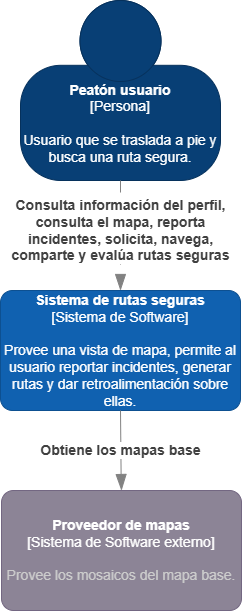
\includegraphics[width=0.3\linewidth]{figures/capitulo6_diseno_sistema/6.1_Arquitectura_del_sistema/diagrama_contexto_sistema.png}
    \caption{Diagrama de contexto del sistema}
    \label{fig:diagrama_contexto}
\end{figure}

\subsection{Diagrama de contenedores}
El diagrama de contenedores descompone el sistema en las aplicaciones y los almacenes de datos que lo conforman, e indica la tecnología utilizada y la comunicación entre ellos \cite{brown_software_architecture}. La figura \ref{fig:diagrama_contenedor} muestra el diagrama correspondiente al presente proyecto.
\begin{figure}[h]
    \centering
    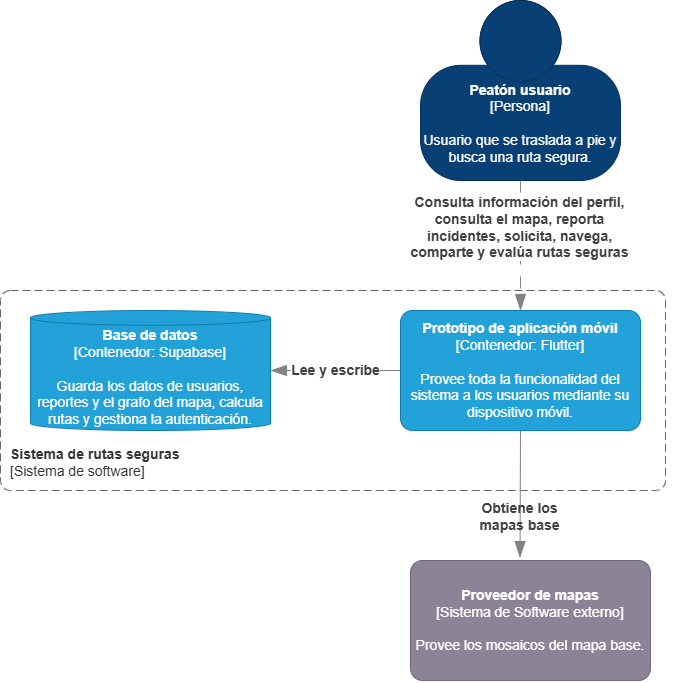
\includegraphics[width=1\linewidth]{figures/capitulo6_diseno_sistema/6.1_Arquitectura_del_sistema/diagrama_contenedor_sistema.png}
    \caption{Diagrama de contenedor del sistema}
    \label{fig:diagrama_contenedor}
\end{figure}

\subsection{Diagrama de componentes}
El diagrama de componentes detalla la estructura interna de un contenedor \cite{brown_software_architecture}. La figura \ref{fig:diagrama_componente} muestra el diagrama correspondiente al presente proyecto.

\clearpage
\newgeometry{landscape, margin=2.5cm}
\begin{figure}[p]
    \centering
    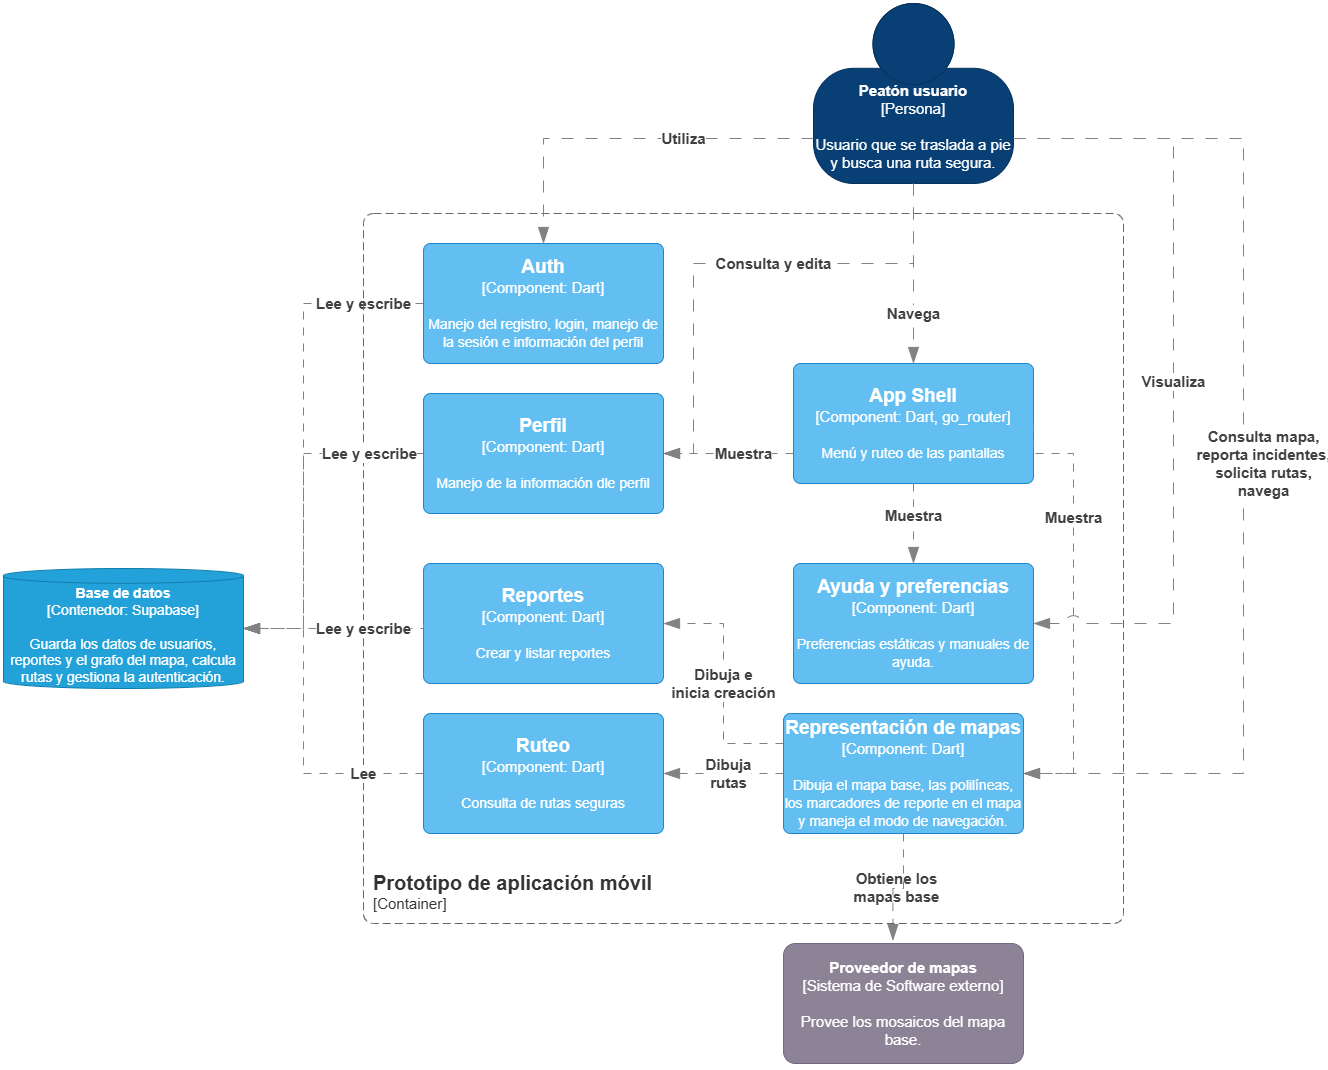
\includegraphics[width=\linewidth, height=1\textheight, keepaspectratio]{figures/capitulo6_diseno_sistema/6.1_Arquitectura_del_sistema/diagrama_componente_sistema.png}
    \caption{Diagrama de contenedor del sistema}
    \label{fig:diagrama_componente}
\end{figure}
\clearpage
\restoregeometry

% =========================================================
% 6.2 CASOS DE USO
% =========================================================
\section{Casos de uso}
\label{sec:casos_uso}
% =========================================================
% 6.2 CASOS DE USO
% El \section{} de esta sección está en el chapter.tex del capítulo;
% sus referencias van en seccion6_2.bib (misma carpeta).
% =========================================================
En esta sección se describen las interacciones de usuarios y sistemas externos con el sistema de generación rutas seguras.

\subsection{Actores}
% =========================================================
% 6.2.1 ACTORES
% Los actores y sus RF coinciden con los diagramas de casos de uso de
% 6.2.2 (figures/capitulo6_diseno_sistema/6.2_Casos_de_uso/cu_*.tex).
% =========================================================
En concordancia con la arquitectura del sistema definida en \ref{sec:arquitectura}, el límite del sistema comprende tanto la aplicación móvil en Flutter como el servicio de base de datos y autenticación en Supabase.

Bajo esta arquitectura, se identifican los siguientes actores primarios (personas) y secundarios (sistemas externos fuera de la frontera del sistema):

\subsubsection{Actores primarios}

\begin{description}
    \item[Usuario no autenticado:] Estado inicial del usuario al interactuar con la aplicación sin una sesión activa o con una cuenta pendiente de verificación. Sus interacciones comprenden el registro de la cuenta con correo electrónico o con una cuenta de Google, la aceptación del aviso de privacidad, la verificación del correo y la solicitud de un nuevo enlace, el inicio de sesión con correo electrónico o con Google, y la recuperación y el restablecimiento de la contraseña mediante un enlace.

    \item[Usuario autenticado:] Usuario con sesión activa que se traslada a pie buscando rutas seguras o que monitorea el trayecto de otros usuarios en tiempo real. Interactúa con todos los módulos de la aplicación para gestionar su perfil y su cuenta, consultar el aviso de privacidad y la sección de ayuda y simbología, activar las notificaciones, administrar sus lugares favoritos, explorar el mapa y sus marcadores, buscar y seleccionar el origen y el destino, solicitar el cálculo de rutas, navegar, registrar, confirmar y desmentir reportes, generar y administrar enlaces y códigos de seguimiento, consultar en el mapa a las personas que sigue e iniciar una llamada de emergencia.
\end{description}

\subsubsection{Actores secundarios (Sistemas externos)}

\begin{description}
    \item[Servicio de correo electrónico:] Servicio externo, implementado con Resend, que envía al usuario los enlaces de verificación del correo y de recuperación de la contraseña, así como sus reenvíos (RF-01, RF-03, RF-10).

    \item[Servicio de identidad de Google:] Servicio externo que autoriza y valida la cuenta de Google del usuario para el registro y el inicio de sesión federados, en comunicación con el servicio de autenticación del sistema (RF-07).

    \item[Servicio de notificaciones push:] Servicio externo, implementado con Firebase Cloud Messaging, que entrega en el dispositivo las alertas de reportes cercanos y los avisos de navegación dirigidos a los seguidores (RF-29, RF-33, RF-35, RF-42).

    \item[Servicio de geocodificación:] Servicio externo, implementado con Geoapify y con Photon como respaldo, que traduce direcciones a coordenadas y coordenadas a texto, y que ofrece el autocompletado para la búsqueda de lugares favoritos y de direcciones de origen y destino (RF-16 a RF-18).

    \item[Servicio de mapas:] Servicio externo, implementado con MapLibre y teselas de OpenFreeMap, que provee el mapa base interactivo y sobre el que se dibujan los marcadores, los trazados de las rutas, la navegación en tiempo real y la ubicación de la persona seguida (\mbox{RF-15}, \mbox{RF-18} a \mbox{RF-20}, \mbox{RF-22}, \mbox{RF-29}, \mbox{RF-31}, \mbox{RF-32}, \mbox{RF-46}).
\end{description}

\begin{table}[htbp]
\centering
\caption{Relación de actores con los requerimientos funcionales del sistema.}
\label{tab:actores_sistema}
\footnotesize
\begin{tabular}{L{3.0cm} L{2.0cm} p{5.6cm} L{2.7cm}}
\hline
\textbf{Actor} & \textbf{Tipo} & \textbf{Descripción en el sistema} & \textbf{RF asociados} \\
\hline
Usuario no autenticado & Primario (Persona) & Registra su cuenta con correo o con Google, acepta el aviso de privacidad, verifica su correo, inicia sesión y recupera su contraseña. & RF-01 a RF-07, RF-10, RF-11, RF-13 \\
\hline
Usuario autenticado & Primario (Persona) & Gestiona su perfil y sus favoritos, explora el mapa, solicita rutas, navega, reporta y valida incidentes, comparte su trayecto, sigue a otros usuarios e inicia llamadas de emergencia. & RF-08, RF-09, RF-12 a RF-38, RF-40 a RF-48 \\
\hline
Servicio de correo electrónico & Secundario (Sistema externo) & Envía los enlaces de verificación y de recuperación de la contraseña. & RF-01, RF-03, RF-10 \\
\hline
Servicio de identidad de Google & Secundario (Sistema externo) & Autoriza y valida la cuenta de Google del usuario. & RF-07 \\
\hline
Servicio de notificaciones push & Secundario (Sistema externo) & Entrega las alertas de reportes cercanos y los avisos de navegación. & RF-29, RF-33, RF-35, RF-42 \\
\hline
Servicio de geocodificación & Secundario (Sistema externo) & Traduce direcciones a coordenadas y viceversa, y autocompleta las búsquedas. & RF-16 a RF-18 \\
\hline
Servicio de mapas & Secundario (Sistema externo) & Provee el mapa base y dibuja marcadores, rutas y posiciones en tiempo real. & RF-15, RF-18 a RF-20, RF-22, RF-29, RF-31, RF-32, RF-46 \\
\hline
\end{tabular}
\end{table}

\subsection{Diagrama de casos de uso}
En esta sección se definen los casos de uso del sistema, los cuales describen las interacciones entre los actores y la aplicación para cumplir los requerimientos funcionales de la sección anterior. Para facilitar su lectura, los casos de uso se organizaron por módulos funcionales, cada uno representado mediante un diagrama de casos de uso de UML. En cada diagrama, las flechas continuas unen a los actores con los casos de uso que utilizan, y las flechas discontinuas indican las relaciones \guillemotleft include\guillemotright{} y \guillemotleft extend\guillemotright{} entre casos de uso.

En la Figura~\ref{fig:casouso1} se presentan los casos de uso del módulo de registro, que comprende el registro de la cuenta con correo electrónico o con una cuenta de Google, la aceptación del aviso de privacidad que ambos incluyen, y la verificación del correo con la opción de solicitar un nuevo enlace. La Figura~\ref{fig:casouso2} muestra los del módulo de autenticación: el inicio de sesión con correo electrónico o con Google, y la recuperación y el restablecimiento de la contraseña mediante un enlace. En la Figura~\ref{fig:casouso3} se muestran los del módulo de perfil y ayuda, que incluye la gestión de la cuenta, la consulta del aviso de privacidad y de la sección de ayuda, y la activación de las notificaciones, y en la Figura~\ref{fig:casouso4} los del módulo de favoritos.

Los casos de uso del módulo de mapas y selección de ubicaciones se presentan en la Figura~\ref{fig:casouso5}, mientras que en la Figura~\ref{fig:casouso6} se muestran los correspondientes al cálculo y selección de rutas. Por su parte, la Figura~\ref{fig:casouso7} muestra los casos de uso de la navegación y los reportes de riesgo, y la Figura~\ref{fig:casouso8} los del módulo de seguridad personal y seguimiento, que abarca la generación y administración de enlaces y códigos de seguimiento, la administración de los seguimientos, la consulta en el mapa de la persona seguida y la llamada de emergencia.

% Los diagramas están dibujados en TikZ (no son imágenes): un archivo por
% módulo en figures/capitulo6_diseno_sistema/6.2_Casos_de_uso/cu_*.tex.
% Estilos en setup/settings.tex, sección G2.
\begin{figure}[htbp]
    \centering
    % =========================================================
% Diagrama de casos de uso: Módulo de Registro  (6.2.2)
% ---------------------------------------------------------
% Estilos: setup/settings.tex, sección G2 (Diagramas de casos de uso).
% CU-04 extiende a CU-03; CU-01 y CU-05 incluyen a CU-02, que queda entre
% ambos. El usuario no se asocia directamente con CU-02.
% =========================================================
\begin{tikzpicture}[node distance=0.35cm]

  % ---------------- Casos de uso ----------------
  \node[cuCaso] (cu04) at (5.4, 0) {CU-04: Solicitar nuevo enlace (RF-03)};
  \node[cuCaso, below=0.9cm of cu04] (cu03) {CU-03: Verificar correo electrónico mediante enlace (RF-02)};
  \node[cuCaso, below=of cu03] (cu01) {CU-01: Registrar cuenta (RF-01)};
  \node[cuCaso, below=0.9cm of cu01] (cu02) {CU-02: Aceptar aviso de privacidad (RF-13)};
  \node[cuCaso, below=0.9cm of cu02] (cu05) {CU-05: Registrarse con cuenta de Google (RF-07)};

  % ---------------- Límite del módulo ----------------
  \node[cuLimiteTitulo, anchor=south] (titulo) at ($(cu04.north)+(0,0.3)$)
    {Módulo de Registro};
  \begin{scope}[on background layer]
    \node[cuLimite, fit=(titulo)(cu04)(cu05)] (limite) {};
  \end{scope}

  % ---------------- Actores ----------------
  % Cada actor externo va a la altura de su caso más bajo: sus líneas llegan
  % de lado o desde arriba y no cruzan el nombre, que va debajo del monito.
  \pic (guest)  at (cu01.north -| 0,0) {cuActor={Usuario no\\autenticado}};
  \pic (email)  at ($(limite.east |- cu01.east)+(3.4,-0.2)$) {cuActorExterno={Servicio de\\correo electrónico}};
  \pic (google) at ($(limite.east |- cu05.east)+(3.4,-0.2)$) {cuActorExterno={Servicio de\\identidad\\de Google}};

  \begin{pgfonlayer}{flechas}
    % ---------------- Asociaciones del usuario ----------------
    \foreach \cu in {cu04, cu03, cu01, cu05}
      \draw[cuAsociacion] (guest-der) -- (\cu.west);

    % ---------------- Inclusiones y extensiones ----------------
    \draw[cuDependencia] (cu04.south) -- (cu03.north)
      node[cuEstereotipo, midway, right] {\guillemotleft extend\guillemotright};
    \draw[cuDependencia] (cu01.south) -- (cu02.north)
      node[cuEstereotipo, midway, right] {\guillemotleft include\guillemotright};
    \draw[cuDependencia] (cu05.north) -- (cu02.south)
      node[cuEstereotipo, midway, right] {\guillemotleft include\guillemotright};

    % ---------------- Sistemas externos ----------------
    \cuExterna{cu04.east}{email}{reenvía enlace\\de verificación}
    \cuExterna{cu01.east}{email}{envía enlace\\de verificación}
    \cuExterna{cu05.east}{google}{autoriza y valida}
  \end{pgfonlayer}

\end{tikzpicture}

    \caption{Diagrama de casos de uso del módulo de registro}
    \label{fig:casouso1}
\end{figure}

\begin{figure}[htbp]
    \centering
    % =========================================================
% Diagrama de casos de uso: Módulo de Autenticación  (6.2.2)
% ---------------------------------------------------------
% Estilos: setup/settings.tex, sección G2 (Diagramas de casos de uso).
% CU-07 extiende a CU-06 y queda justo encima de él; el caso de Google
% (CU-10) va al final, junto a su sistema externo.
% =========================================================
\begin{tikzpicture}[node distance=0.35cm]

  % ---------------- Casos de uso ----------------
  \node[cuCaso] (cu07) at (5.4, 0) {CU-07: Solicitar nuevo enlace (RF-04)};
  \node[cuCaso, below=0.9cm of cu07] (cu06) {CU-06: Solicitar recuperación de contraseña mediante enlace (RF-10)};
  \node[cuCaso, below=of cu06] (cu08) {CU-08: Restablecer contraseña mediante enlace (RF-11)};
  \node[cuCaso, below=of cu08] (cu09) {CU-09: Iniciar sesión con correo electrónico (RF-06)};
  \node[cuCaso, below=of cu09] (cu10) {CU-10: Iniciar sesión con cuenta de Google (RF-07)};

  % ---------------- Límite del módulo ----------------
  \node[cuLimiteTitulo, anchor=south] (titulo) at ($(cu07.north)+(0,0.3)$)
    {Módulo de Autenticación};
  \begin{scope}[on background layer]
    \node[cuLimite, fit=(titulo)(cu07)(cu10)] (limite) {};
  \end{scope}

  % ---------------- Actores ----------------
  % Cada actor externo va a la altura de su caso más bajo: sus líneas llegan
  % de lado o desde arriba y no cruzan el nombre, que va debajo del monito.
  \pic (guest)  at (cu08.north -| 0,0) {cuActor={Usuario no\\autenticado}};
  \pic (email)  at ($(limite.east |- cu06.east)+(3.4,-0.2)$) {cuActorExterno={Servicio de\\correo electrónico}};
  \pic (google) at ($(limite.east |- cu10.east)+(3.4,-0.2)$) {cuActorExterno={Servicio de\\identidad\\de Google}};

  \begin{pgfonlayer}{flechas}
    % ---------------- Asociaciones del usuario ----------------
    \foreach \cu in {cu07, cu06, cu08, cu09, cu10}
      \draw[cuAsociacion] (guest-der) -- (\cu.west);

    % ---------------- Extensión ----------------
    \draw[cuDependencia] (cu07.south) -- (cu06.north)
      node[cuEstereotipo, midway, right] {\guillemotleft extend\guillemotright};

    % ---------------- Sistemas externos ----------------
    \cuExterna{cu06.east}{email}{envía enlace\\de recuperación}
    \cuExterna{cu10.east}{google}{autoriza y valida}
  \end{pgfonlayer}

\end{tikzpicture}

    \caption{Diagrama de casos de uso del módulo de autenticación}
    \label{fig:casouso2}
\end{figure}

\begin{figure}[htbp]
    \centering
    % =========================================================
% Diagrama de casos de uso: Módulo de Perfil y Ayuda  (6.2.2)
% ---------------------------------------------------------
% Estilos: setup/settings.tex, sección G2 (Diagramas de casos de uso).
% Solo CU-17 usa un sistema externo; va al final, junto a él.
% =========================================================
\begin{tikzpicture}[node distance=0.35cm]

  % ---------------- Casos de uso ----------------
  \node[cuCaso] (cu11) at (5.4, 0) {CU-11: Cambiar contraseña (RF-09)};
  \node[cuCaso, below=of cu11] (cu12) {CU-12: Cerrar sesión (RF-08)};
  \node[cuCaso, below=of cu12] (cu13) {CU-13: Eliminar cuenta (RF-12)};
  \node[cuCaso, below=of cu13] (cu14) {CU-14: Consultar el aviso de privacidad (RF-13)};
  \node[cuCaso, below=of cu14] (cu15) {CU-15: Consultar sección de ayuda y simbología (RF-48)};
  \node[cuCaso, below=of cu15] (cu16) {CU-16: Editar datos del perfil (RF-14)};
  \node[cuCaso, below=of cu16] (cu17) {CU-17: Activar notificaciones (RF-42)};

  % ---------------- Límite del módulo ----------------
  \node[cuLimiteTitulo, anchor=south] (titulo) at ($(cu11.north)+(0,0.3)$)
    {Módulo de Perfil y Ayuda};
  \begin{scope}[on background layer]
    \node[cuLimite, fit=(titulo)(cu11)(cu17)] (limite) {};
  \end{scope}

  % ---------------- Actores ----------------
  \pic (user) at (cu14.north -| 0,0) {cuActor={Usuario\\autenticado}};
  \pic (push) at ($(limite.east |- cu17.east)+(3.4,-0.2)$) {cuActorExterno={Servicio de\\notificaciones push}};

  \begin{pgfonlayer}{flechas}
    \foreach \cu in {cu11, cu12, cu13, cu14, cu15, cu16, cu17}
      \draw[cuAsociacion] (user-der) -- (\cu.west);

    % ---------------- Sistema externo ----------------
    \cuExterna{cu17.east}{push}{envía alertas}
  \end{pgfonlayer}

\end{tikzpicture}

    \caption{Diagrama de casos de uso del módulo de perfil y ayuda}
    \label{fig:casouso3}
\end{figure}

\begin{figure}[htbp]
    \centering
    % =========================================================
% Diagrama de casos de uso: Módulo de Favoritos  (6.2.2)
% ---------------------------------------------------------
% Estilos: setup/settings.tex, sección G2 (Diagramas de casos de uso).
% CU-18, CU-20 y CU-21 extienden a CU-19. CU-18 y CU-20 quedan junto a
% CU-19; la extensión de CU-21 rodea a CU-20 por la izquierda, por debajo
% de las flechas del usuario, para no cruzar ninguna línea.
% =========================================================
\begin{tikzpicture}[node distance=0.35cm]

  % ---------------- Casos de uso ----------------
  \node[cuCaso] (cu18) at (5.4, 0) {CU-18: Agregar lugar favorito (RF-18)};
  \node[cuCaso, below=1.3cm of cu18] (cu19) {CU-19: Consultar lugares favoritos (RF-18)};
  \node[cuCaso, below=0.9cm of cu19] (cu20) {CU-20: Editar lugares favoritos (RF-18)};
  \node[cuCaso, below=of cu20] (cu21) {CU-21: Eliminar lugares favoritos (RF-18)};

  % ---------------- Límite del módulo ----------------
  \node[cuLimiteTitulo, anchor=south] (titulo) at ($(cu18.north)+(0,0.3)$)
    {Módulo de Favoritos};
  \begin{scope}[on background layer]
    \node[cuLimite, fit=(titulo)(cu18)(cu21)] (limite) {};
  \end{scope}

  % ---------------- Actores ----------------
  % Cada actor externo va a la altura de su caso más bajo: sus líneas llegan
  % de lado o desde arriba y no cruzan el nombre, que va debajo del monito.
  \pic (user)  at (cu19.north -| 0,0) {cuActor={Usuario\\autenticado}};
  % Geocodificación más arriba: la línea CU-18 -> mapas pasa por debajo de su nombre
  \pic (geo)   at ($(limite.east |- cu18.east)+(3.4,0.8)$) {cuActorExterno={Servicio de\\geocodificación}};
  \pic (mapas) at ($(limite.east |- cu19.east)+(3.4,-0.2)$) {cuActorExterno={Servicio\\de mapas}};

  \begin{pgfonlayer}{flechas}
    % ---------------- Asociaciones del usuario ----------------
    \foreach \cu in {cu18, cu19}
      \draw[cuAsociacion] (user-der) -- (\cu.west);

    % ---------------- Extensiones ----------------
    \draw[cuDependencia] (cu18.south) -- (cu19.north)
      node[cuEstereotipo, midway, right] {\guillemotleft extend\guillemotright};
    \draw[cuDependencia] (cu20.north) -- (cu19.south)
      node[cuEstereotipo, midway, right] {\guillemotleft extend\guillemotright};
    \draw[cuDependencia, rounded corners=6pt]
      (cu21.west) -- ++(-0.45,0) |- ($(cu19.south west)!0.5!(cu19.west)$)
      node[cuEstereotipo, pos=0.25, left] {\guillemotleft extend\guillemotright};

    % ---------------- Sistemas externos ----------------
    \cuExterna[xshift=-0.6cm, yshift=0.15cm]{cu18.east}{geo}{traduce\\dirección a\\coordenadas}
    \cuExterna{cu18.south east}{mapas}{selecciona punto}
    \cuExterna{cu19.east}{mapas}{renderiza puntos}
  \end{pgfonlayer}

\end{tikzpicture}

    \caption{Diagrama de casos de uso del módulo de favoritos}
    \label{fig:casouso4}
\end{figure}

\begin{figure}[htbp]
    \centering
    % =========================================================
% Diagrama de casos de uso: Módulo de Mapas y Selección de Ubicaciones  (6.2.2)
% ---------------------------------------------------------
% Estilos: setup/settings.tex, sección G2 (Diagramas de casos de uso).
% Tres casos (CU-22 a CU-24) usan el servicio de mapas y dos (CU-25,
% CU-26) el de geocodificación. Como varias líneas llegan al mismo actor,
% sus textos no van en el centro del hueco (\cuExterna) sino más cerca de
% cada caso, donde las líneas aún están separadas; los casos de cada grupo
% van más espaciados para que ninguna línea pase por detrás de otro texto.
% =========================================================
\begin{tikzpicture}[node distance=0.35cm]

  % ---------------- Casos de uso ----------------
  \node[cuCaso] (cu22) at (5.4, 0) {CU-22: Visualizar puntos de ayuda (RF-19)};
  \node[cuCaso, below=2.3cm of cu22] (cu23) {CU-23: Interactuar con el mapa base (RF-15)};
  \node[cuCaso, below=2.0cm of cu23] (cu24) {CU-24: Visualizar reportes validados (RF-20)};
  \node[cuCaso, below=0.6cm of cu24] (cu25) {CU-25: Buscar origen y destino (RF-16)};
  \node[cuCaso, below=3.3cm of cu25] (cu26) {CU-26: Seleccionar origen y destino en el mapa (RF-17)};

  % ---------------- Límite del módulo ----------------
  \node[cuLimiteTitulo, anchor=south] (titulo) at ($(cu22.north)+(0,0.3)$)
    {Módulo de Mapas y Selección de Ubicaciones};
  \begin{scope}[on background layer]
    \node[cuLimite, fit=(titulo)(cu22)(cu26)] (limite) {};
  \end{scope}

  % ---------------- Actores ----------------
  % Cada actor externo va a la altura de su caso más bajo: sus líneas llegan
  % de lado o desde arriba y no cruzan el nombre, que va debajo del monito.
  \pic (user)  at (cu24.north -| 0,0) {cuActor={Usuario\\autenticado}};
  \pic (mapas) at ($(limite.east |- cu24.east)+(3.4,-0.2)$) {cuActorExterno={Servicio\\de mapas}};
  \pic (geo)   at ($(limite.east |- cu26.east)+(3.4,-0.2)$) {cuActorExterno={Servicio de\\geocodificación}};

  \begin{pgfonlayer}{flechas}
    % ---------------- Asociaciones del usuario ----------------
    \foreach \cu in {cu22, cu23, cu24, cu25, cu26}
      \draw[cuAsociacion] (user-der) -- (\cu.west);

    % ---------------- Sistemas externos ----------------
    \draw[cuAsociacion] (cu22.east) -- (mapas-izq)
      node[cuEtiqueta, pos=0.4] {dibuja\\marcadores};
    \draw[cuAsociacion] (cu23.east) -- (mapas-izq)
      node[cuEtiqueta, pos=0.41] {solicita\\renderizado\\del mapa};
    \draw[cuAsociacion] (cu24.east) -- (mapas-izq)
      node[cuEtiqueta, pos=0.55] {dibuja\\marcadores};
    \draw[cuAsociacion] (cu25.east) -- (geo-izq)
      node[cuEtiqueta, pos=0.56] {autocompletado y\\geocodificación};
    \draw[cuAsociacion] (cu26.east) -- (geo-izq)
      node[cuEtiqueta, pos=0.48] {geocodificación\\inversa\\(coordenadas\\a texto)};
  \end{pgfonlayer}

\end{tikzpicture}

    \caption{Diagrama de casos de uso del módulo de mapas y selección de ubicaciones}
    \label{fig:casouso5}
\end{figure}

\begin{figure}[htbp]
    \centering
    % =========================================================
% Diagrama de casos de uso: Módulo de Cálculo y Selección de Rutas  (6.2.2)
% ---------------------------------------------------------
% Estilos: setup/settings.tex, sección G2 (Diagramas de casos de uso).
% CU-27 incluye a CU-28; CU-29 y CU-30 lo extienden. La extensión de
% CU-30 rodea a CU-29 por la izquierda, por debajo de las flechas del
% usuario. CU-30 usa dos sistemas externos: el servicio push queda a su
% altura y el de mapas arriba, junto a CU-27; la línea de CU-30 llega al
% pie del nombre del servicio de mapas para no cruzarlo.
% =========================================================
\begin{tikzpicture}[node distance=0.35cm]

  % ---------------- Casos de uso ----------------
  \node[cuCaso] (cu27) at (5.4, 0) {CU-27: Solicitar cálculo de rutas (RF-21, RF-22, RF-26, RF-27, RF-28)};
  \node[cuCaso, below=0.9cm of cu27] (cu28) {CU-28: Consultar resumen y riesgo de las rutas (RF-23, RF-24)};
  \node[cuCaso, below=0.9cm of cu28] (cu29) {CU-29: Consultar detalle de una ruta específica (RF-25)};
  \node[cuCaso, below=of cu29] (cu30) {CU-30: Seleccionar ruta e iniciar navegación (RF-29)};

  % ---------------- Límite del módulo ----------------
  \node[cuLimiteTitulo, anchor=south] (titulo) at ($(cu27.north)+(0,0.3)$)
    {Módulo de Cálculo y Selección de Rutas};
  \begin{scope}[on background layer]
    \node[cuLimite, fit=(titulo)(cu27)(cu30)] (limite) {};
  \end{scope}

  % ---------------- Actores ----------------
  \pic (user)  at (cu28.north -| 0,0) {cuActor={Usuario\\autenticado}};
  \pic (mapas) at ($(limite.east |- cu27.east)+(3.4,-0.2)$) {cuActorExterno={Servicio\\de mapas}};
  \pic (push)  at ($(limite.east |- cu30.east)+(3.4,-0.2)$) {cuActorExterno={Servicio de\\notificaciones push}};

  \begin{pgfonlayer}{flechas}
    % ---------------- Asociaciones del usuario ----------------
    \foreach \cu in {cu27, cu28}
      \draw[cuAsociacion] (user-der) -- (\cu.west);

    % ---------------- Inclusión y extensiones ----------------
    \draw[cuDependencia] (cu27.south) -- (cu28.north)
      node[cuEstereotipo, midway, right] {\guillemotleft include\guillemotright};
    \draw[cuDependencia] (cu29.north) -- (cu28.south)
      node[cuEstereotipo, midway, right] {\guillemotleft extend\guillemotright};
    \draw[cuDependencia, rounded corners=6pt]
      (cu30.west) -- ++(-0.45,0) |- ($(cu28.south west)!0.5!(cu28.west)$)
      node[cuEstereotipo, pos=0.25, left] {\guillemotleft extend\guillemotright};

    % ---------------- Sistemas externos ----------------
    \cuExterna{cu27.east}{mapas}{obtiene trazados\\y distancias}
    \draw[cuAsociacion] (cu30.north east) -- (mapas-nombre.south)
      node[cuEtiqueta, pos=0.6] {renderiza la\\navegación en\\tiempo real};
    \cuExterna{cu30.east}{push}{envía notificación}
  \end{pgfonlayer}

\end{tikzpicture}

    \caption{Diagrama de casos de uso del módulo de cálculo y selección de rutas}
    \label{fig:casouso6}
\end{figure}

\begin{figure}[htbp]
    \centering
    % =========================================================
% Diagrama de casos de uso: Módulo de Navegación y Reportes  (6.2.2)
% ---------------------------------------------------------
% Estilos: setup/settings.tex, sección G2 (Diagramas de casos de uso).
% CU-35 extiende a CU-34 y queda justo debajo de él.
% =========================================================
\begin{tikzpicture}[node distance=0.35cm]

  % ---------------- Casos de uso ----------------
  \node[cuCaso] (cu31) at (5.4, 0) {CU-31: Visualizar posición y avance en el mapa (RF-31, RF-32)};
  \node[cuCaso, below=of cu31] (cu32) {CU-32: Registrar reporte de riesgo (RF-37, RF-38)};
  \node[cuCaso, below=of cu32] (cu33) {CU-33: Pausar, reanudar y cancelar navegación (RF-33, RF-35)};
  \node[cuCaso, below=of cu33] (cu34) {CU-34: Consultar reportes pendientes cercanos (RF-40)};
  \node[cuCaso, below=0.9cm of cu34] (cu35) {CU-35: Confirmar o desmentir reporte de otro usuario (RF-41)};

  % ---------------- Límite del módulo ----------------
  \node[cuLimiteTitulo, anchor=south] (titulo) at ($(cu31.north)+(0,0.3)$)
    {Módulo de Navegación y Reportes};
  \begin{scope}[on background layer]
    \node[cuLimite, fit=(titulo)(cu31)(cu35)] (limite) {};
  \end{scope}

  % ---------------- Actores ----------------
  % Cada actor externo va a la altura de su caso más bajo: sus líneas llegan
  % de lado o desde arriba y no cruzan el nombre, que va debajo del monito.
  \pic (user)  at (cu33.north -| 0,0) {cuActor={Usuario\\autenticado}};
  \pic (mapas) at ($(limite.east |- cu31.east)+(3.4,-0.2)$) {cuActorExterno={Servicio\\de mapas}};
  \pic (push)  at ($(limite.east |- cu33.east)+(3.4,-0.2)$) {cuActorExterno={Servicio de\\notificaciones push}};

  \begin{pgfonlayer}{flechas}
    % ---------------- Asociaciones del usuario ----------------
    \foreach \cu in {cu31, cu32, cu33, cu34}
      \draw[cuAsociacion] (user-der) -- (\cu.west);

    % ---------------- Extensión ----------------
    \draw[cuDependencia] (cu35.north) -- (cu34.south)
      node[cuEstereotipo, midway, right] {\guillemotleft extend\guillemotright};

    % ---------------- Sistemas externos ----------------
    \cuExterna{cu31.east}{mapas}{renderiza la ruta\\o el mapa}
    \cuExterna{cu33.east}{push}{envía notificación}
  \end{pgfonlayer}

\end{tikzpicture}

    \caption{Diagrama de casos de uso del módulo de navegación y reportes}
    \label{fig:casouso7}
\end{figure}

\begin{figure}[htbp]
    \centering
    % =========================================================
% Diagrama de casos de uso: Módulo de Seguridad Personal y Seguimiento  (6.2.2)
% ---------------------------------------------------------
% Estilos: setup/settings.tex, sección G2 (Diagramas de casos de uso).
% CU-41 extiende a CU-40 y queda justo debajo de él.
% =========================================================
\begin{tikzpicture}[node distance=0.35cm]

  % ---------------- Casos de uso ----------------
  \node[cuCaso] (cu37) at (5.4, 0) {CU-37: Generar y compartir enlace o código (RF-43)};
  \node[cuCaso, below=of cu37] (cu38) {CU-38: Iniciar llamada de emergencia (RF-47)};
  \node[cuCaso, below=of cu38] (cu39) {CU-39: Administrar «Mis enlaces» (RF-44)};
  \node[cuCaso, below=of cu39] (cu40) {CU-40: Administrar «Mis seguimientos» (RF-45)};
  \node[cuCaso, below=0.9cm of cu40] (cu41) {CU-41: Visualizar en el mapa a la persona seguida (RF-46)};

  % ---------------- Límite del módulo ----------------
  \node[cuLimiteTitulo, anchor=south] (titulo) at ($(cu37.north)+(0,0.3)$)
    {Módulo de Seguridad Personal y Seguimiento};
  \begin{scope}[on background layer]
    \node[cuLimite, fit=(titulo)(cu37)(cu41)] (limite) {};
  \end{scope}

  % ---------------- Actores ----------------
  \pic (user)  at (cu39.north -| 0,0) {cuActor={Usuario\\autenticado}};
  \pic (mapas) at ($(limite.east |- cu41.east)+(3.4,-0.2)$) {cuActorExterno={Servicio\\de mapas}};

  \begin{pgfonlayer}{flechas}
    % ---------------- Asociaciones del usuario ----------------
    \foreach \cu in {cu37, cu38, cu39, cu40}
      \draw[cuAsociacion] (user-der) -- (\cu.west);

    % ---------------- Extensión ----------------
    \draw[cuDependencia] (cu41.north) -- (cu40.south)
      node[cuEstereotipo, midway, right] {\guillemotleft extend\guillemotright};

    % ---------------- Sistema externo ----------------
    \cuExterna{cu41.east}{mapas}{renderiza\\ubicación en\\tiempo real}
  \end{pgfonlayer}

\end{tikzpicture}

    \caption{Diagrama de casos de uso del módulo de seguridad personal y seguimiento}
    \label{fig:casouso8}
\end{figure}

\subsection{Especificación de casos de uso}
% =========================================================
% 6.2.3 Especificación de casos de uso
% Requiere \input{cu_especificacion_preambulo} en el preámbulo.
% =========================================================
En esta sección se especifica cada caso de uso de los diagramas anteriores. Cada especificación indica los actores que participan, los requerimientos y reglas de negocio que cubre, las condiciones para iniciarlo, el flujo principal, los flujos alternativos (FA), las condiciones al terminar y sus relaciones con otros casos de uso. Los casos incluidos que no tienen número propio, como la validación del área de servicio, se describen dentro del flujo del caso que los incluye.

% ---------------------------------------------------------
\paragraph{Diagrama 1: Módulo de Acceso y Autenticación}\mbox{}

\begin{especificacionCU}{CU-01}{Aceptar aviso de privacidad inicial}
  \cuCampo{Actores}{Peatón usuario (No autenticado).}
  \cuCampo{Requerimientos}{RF-12.}
  \cuCampo{Reglas de negocio}{RN-16.}
  \cuCampo{Descripción}{En el primer uso, el sistema presenta el aviso de privacidad y registra el consentimiento del usuario antes de permitir el registro de una cuenta.}
  \cuCampo{Precondiciones}{Es el primer uso de la aplicación y el consentimiento aún no está registrado.}
  \cuPasos{Flujo principal}{
    \item El usuario inicia el registro de una cuenta (CU-02 o CU-06).
    \item El sistema presenta el aviso de privacidad, que describe el uso de la ubicación conforme a RN-16.
    \item El usuario lee el aviso y lo acepta.
    \item El sistema registra el consentimiento del usuario.
    \item El sistema regresa al caso de uso que lo incluyó.
  }
  \cuCampo{Flujos alternativos}{\textbf{FA-1 El usuario no acepta el aviso.} En el paso 3, si el usuario rechaza o cierra el aviso, el sistema no registra el consentimiento, informa que es necesario aceptarlo para crear una cuenta y no permite continuar con el registro. El caso termina.}
  \cuCampo{Postcondiciones}{El consentimiento queda registrado conforme a RN-16.}
  \cuCampo{Relaciones}{Incluido por CU-02 y CU-06.}
\end{especificacionCU}

\begin{especificacionCU}{CU-02}{Registrar cuenta con correo electrónico}
  \cuCampo{Actores}{Peatón usuario (No autenticado).}
  \cuCampo{Requerimientos}{RF-01, RF-02.}
  \cuCampo{Reglas de negocio}{RN-14, RN-16, RN-17.}
  \cuCampo{Descripción}{El usuario crea una cuenta con su correo electrónico y una contraseña; la cuenta queda pendiente de verificación.}
  \cuCampo{Precondiciones}{El dispositivo tiene conexión a internet.}
  \cuPasos{Flujo principal}{
    \item El usuario selecciona la opción de registrarse.
    \item El sistema incluye CU-01 si el consentimiento del aviso de privacidad no está registrado.
    \item El sistema muestra el formulario de registro.
    \item El usuario captura su correo electrónico y su contraseña, y confirma el registro.
    \item El sistema verifica que los datos sean válidos y que el correo no esté asociado a otra cuenta.
    \item El sistema registra la cuenta en estado no verificado y almacena la contraseña conforme a RNF-14.
    \item El sistema envía al correo un enlace de verificación de un solo uso, vigente durante 10 minutos (RF-02, RN-14).
    \item El sistema muestra el aviso de verificación pendiente.
  }
  \cuCampo{Flujos alternativos}{\textbf{FA-1 Correo ya registrado.} En el paso 5, si el correo pertenece a otra cuenta, el sistema lo informa conforme a RNF-10 y ofrece iniciar sesión o recuperar la contraseña. Regresa al paso 4.\par\smallskip
    \textbf{FA-2 Datos incompletos o inválidos.} En el paso 5, si falta un dato o tiene un formato inválido, el sistema señala el campo con un mensaje conforme a RNF-10. Regresa al paso 4.\par\smallskip
    \textbf{FA-3 Sin conexión a internet.} En el paso 4, si el dispositivo no tiene conexión, el sistema informa la condición conforme a RNF-10 y no registra la cuenta. El caso termina.}
  \cuCampo{Postcondiciones}{La cuenta queda registrada en estado no verificado y el enlace de verificación queda enviado al correo del usuario.}
  \cuCampo{Relaciones}{Incluye CU-01.}
\end{especificacionCU}

\begin{especificacionCU}{CU-03}{Verificar correo electrónico}
  \cuCampo{Actores}{Peatón usuario (No autenticado).}
  \cuCampo{Requerimientos}{RF-02.}
  \cuCampo{Reglas de negocio}{RN-14, RN-17.}
  \cuCampo{Descripción}{El usuario confirma que el correo registrado le pertenece al abrir el enlace de verificación.}
  \cuCampo{Precondiciones}{La cuenta está registrada sin verificar y el usuario recibió el enlace de verificación (CU-02 o CU-04).}
  \cuPasos{Flujo principal}{
    \item El usuario abre el enlace de verificación recibido en su correo.
    \item El sistema comprueba que el enlace no se haya usado y que no hayan transcurrido más de 10 minutos desde su emisión (RN-14).
    \item El sistema marca la cuenta como verificada e invalida el enlace.
    \item El sistema informa que la verificación fue exitosa y muestra la pantalla de inicio de sesión.
  }
  \cuCampo{Flujos alternativos}{\textbf{FA-1 Enlace expirado o usado.} En el paso 2, si el enlace ya se usó o expiró, el sistema lo informa conforme a RNF-10 y ofrece solicitar un nuevo enlace (CU-04). El caso termina.}
  \cuCampo{Postcondiciones}{La cuenta queda verificada y el usuario puede usar todas las funciones de la aplicación (RN-17).}
  \cuCampo{Relaciones}{Ninguna.}
\end{especificacionCU}

\begin{especificacionCU}{CU-04}{Solicitar reenvío de enlace de verificación}
  \cuCampo{Actores}{Peatón usuario (No autenticado).}
  \cuCampo{Requerimientos}{RF-03, RF-04.}
  \cuCampo{Reglas de negocio}{RN-14, RN-17.}
  \cuCampo{Descripción}{Desde el aviso de verificación pendiente, el usuario solicita un nuevo enlace de verificación.}
  \cuCampo{Precondiciones}{La cuenta está registrada sin verificar y el dispositivo tiene conexión a internet.}
  \cuPasos{Flujo principal}{
    \item En el punto de extensión \enquote{Cuenta no verificada} de CU-05, el sistema muestra el aviso de verificación pendiente.
    \item El usuario selecciona la opción de reenviar el enlace.
    \item El sistema genera un nuevo enlace de un solo uso, vigente durante 10 minutos (RN-14).
    \item El sistema envía el nuevo enlace al correo registrado y confirma el envío.
  }
  \cuCampo{Flujos alternativos}{\textbf{FA-1 Sin conexión a internet.} En el paso 2, si el dispositivo no tiene conexión, el sistema informa la condición conforme a RNF-10 y no envía el enlace. El caso termina.}
  \cuCampo{Postcondiciones}{Un nuevo enlace de verificación queda enviado al correo del usuario.}
  \cuCampo{Relaciones}{Extiende CU-05 en el punto de extensión \enquote{Cuenta no verificada}, cuando la cuenta no está verificada (RF-04).}
\end{especificacionCU}

\begin{especificacionCU}{CU-05}{Iniciar sesión con correo electrónico}
  \cuCampo{Actores}{Peatón usuario (No autenticado).}
  \cuCampo{Requerimientos}{RF-05, RF-04.}
  \cuCampo{Reglas de negocio}{RN-17.}
  \cuCampo{Descripción}{El usuario accede a la aplicación con su correo electrónico y su contraseña.}
  \cuCampo{Precondiciones}{El usuario tiene una cuenta registrada con correo y contraseña, y el dispositivo tiene conexión a internet.}
  \cuPasos{Flujo principal}{
    \item El usuario captura su correo electrónico y su contraseña y selecciona la opción de entrar.
    \item El sistema valida las credenciales.
    \item El sistema comprueba que la cuenta esté verificada (RN-17).
    \item El sistema inicia la sesión y muestra la pantalla principal.
  }
  \cuCampo{Flujos alternativos}{\textbf{FA-1 Credenciales incorrectas.} En el paso 2, si el correo o la contraseña son incorrectos, el sistema lo informa conforme a RNF-10. Regresa al paso 1.\par\smallskip
    \textbf{FA-2 Cuenta no verificada.} En el paso 3, si la cuenta no está verificada, el sistema deniega el acceso y muestra el aviso de verificación pendiente con la opción de reenviar el enlace (RF-04). El caso termina.\par\smallskip
    \textbf{FA-3 Sin conexión a internet.} En el paso 1, si el dispositivo no tiene conexión, el sistema informa la condición conforme a RNF-10. El caso termina.}
  \cuCampo{Postcondiciones}{La sesión del usuario queda activa y se muestra la pantalla principal.}
  \cuCampo{Relaciones}{Extendido por CU-04 en el punto de extensión \enquote{Cuenta no verificada} (paso 3).}
\end{especificacionCU}

\begin{especificacionCU}{CU-06}{Autenticar con cuenta de Google}
  \cuCampo{Actores}{Peatón usuario (No autenticado) (principal); Proveedor de identidad de Google (secundario).}
  \cuCampo{Requerimientos}{RF-06, RF-12.}
  \cuCampo{Reglas de negocio}{RN-16, RN-17.}
  \cuCampo{Descripción}{El usuario se registra o inicia sesión con su cuenta de Google, sin requerir la verificación del correo.}
  \cuCampo{Precondiciones}{El usuario tiene una cuenta de Google y el dispositivo tiene conexión a internet.}
  \cuPasos{Flujo principal}{
    \item El usuario selecciona la opción \enquote{Continuar con Google}.
    \item El sistema incluye CU-01 si el consentimiento del aviso de privacidad no está registrado.
    \item El sistema solicita la autorización al Proveedor de identidad de Google.
    \item El usuario elige su cuenta de Google y autoriza el acceso.
    \item El Proveedor de identidad de Google valida las credenciales y devuelve la identidad del usuario.
    \item Si no existe una cuenta con ese correo, el sistema crea una cuenta vinculada a Google que no requiere verificación (RN-17).
    \item El sistema inicia la sesión y muestra la pantalla principal.
  }
  \cuCampo{Flujos alternativos}{\textbf{FA-1 Correo ya registrado con contraseña.} En el paso 6, si el correo de Google ya pertenece a una cuenta con contraseña, el sistema vincula ambas formas de acceso a la misma cuenta. Continúa en el paso 7.\par\smallskip
    \textbf{FA-2 Autorización cancelada o rechazada.} En el paso 4 o 5, si el usuario cancela o Google rechaza la autorización, el sistema no inicia la sesión y regresa a la pantalla de inicio de sesión. El caso termina.\par\smallskip
    \textbf{FA-3 Sin conexión a internet.} En el paso 1, si el dispositivo no tiene conexión, el sistema informa la condición conforme a RNF-10. El caso termina.}
  \cuCampo{Postcondiciones}{La sesión del usuario queda activa y vinculada a su cuenta de Google.}
  \cuCampo{Relaciones}{Incluye CU-01.}
\end{especificacionCU}

\begin{especificacionCU}{CU-07}{Solicitar recuperación de contraseña}
  \cuCampo{Actores}{Peatón usuario (No autenticado).}
  \cuCampo{Requerimientos}{RF-09.}
  \cuCampo{Reglas de negocio}{RN-14.}
  \cuCampo{Descripción}{El usuario solicita un enlace para restablecer su contraseña.}
  \cuCampo{Precondiciones}{El dispositivo tiene conexión a internet.}
  \cuPasos{Flujo principal}{
    \item El usuario selecciona la opción \enquote{¿Olvidaste tu contraseña?} en la pantalla de inicio de sesión.
    \item El sistema solicita el correo electrónico de la cuenta.
    \item El usuario captura su correo y confirma la solicitud.
    \item El sistema genera un enlace de restablecimiento de un solo uso, vigente durante 10 minutos (RN-14), y lo envía al correo.
    \item El sistema confirma que el enlace fue enviado.
  }
  \cuCampo{Flujos alternativos}{\textbf{FA-1 Correo no registrado.} En el paso 4, si el correo no pertenece a una cuenta con contraseña, el sistema muestra la misma confirmación del paso 5 sin enviar ningún enlace, de modo que no se revele qué correos están registrados.\par\smallskip
    \textbf{FA-2 Sin conexión a internet.} En el paso 3, si el dispositivo no tiene conexión, el sistema informa la condición conforme a RNF-10. El caso termina.}
  \cuCampo{Postcondiciones}{El enlace de restablecimiento queda enviado al correo del usuario.}
  \cuCampo{Relaciones}{Ninguna. El restablecimiento continúa en CU-08.}
\end{especificacionCU}

\begin{especificacionCU}{CU-08}{Restablecer contraseña}
  \cuCampo{Actores}{Peatón usuario (No autenticado).}
  \cuCampo{Requerimientos}{RF-10.}
  \cuCampo{Reglas de negocio}{RN-14.}
  \cuCampo{Descripción}{El usuario establece una nueva contraseña mediante el enlace de restablecimiento.}
  \cuCampo{Precondiciones}{El usuario recibió un enlace de restablecimiento (CU-07) y el dispositivo tiene conexión a internet.}
  \cuPasos{Flujo principal}{
    \item El usuario abre el enlace de restablecimiento.
    \item El sistema comprueba que el enlace no se haya usado y que no haya expirado (RN-14).
    \item El sistema solicita la nueva contraseña y su confirmación.
    \item El usuario captura la nueva contraseña y la confirma.
    \item El sistema registra la nueva contraseña conforme a RNF-14 e invalida el enlace.
    \item El sistema confirma el cambio y muestra la pantalla de inicio de sesión.
  }
  \cuCampo{Flujos alternativos}{\textbf{FA-1 Enlace expirado o usado.} En el paso 2, si el enlace ya se usó o expiró, el sistema lo informa conforme a RNF-10 y ofrece solicitar uno nuevo (CU-07). El caso termina.\par\smallskip
    \textbf{FA-2 Las contraseñas no coinciden.} En el paso 4, si la confirmación no coincide con la nueva contraseña, el sistema lo informa. Regresa al paso 3.}
  \cuCampo{Postcondiciones}{La nueva contraseña queda registrada, el enlace queda invalidado y se muestra la pantalla de inicio de sesión.}
  \cuCampo{Relaciones}{Ninguna.}
\end{especificacionCU}

% ---------------------------------------------------------
\paragraph{Diagrama 2: Módulo de Perfil y Ayuda}\mbox{}

\begin{especificacionCU}{CU-09}{Cambiar contraseña}
  \cuCampo{Actores}{Peatón usuario (Autenticado).}
  \cuCampo{Requerimientos}{RF-08.}
  \cuCampo{Reglas de negocio}{Ninguna.}
  \cuCampo{Descripción}{El usuario reemplaza su contraseña indicando la contraseña vigente.}
  \cuCampo{Precondiciones}{El usuario tiene una sesión iniciada con una cuenta de correo y contraseña, y el dispositivo tiene conexión a internet.}
  \cuPasos{Flujo principal}{
    \item El usuario selecciona la opción \enquote{Cambiar contraseña} en el perfil.
    \item El sistema solicita la contraseña vigente, la nueva contraseña y su confirmación.
    \item El usuario captura los datos y confirma el cambio.
    \item El sistema verifica que la contraseña vigente sea correcta.
    \item El sistema registra la nueva contraseña conforme a RNF-14; la anterior deja de ser válida.
    \item El sistema confirma el cambio.
  }
  \cuCampo{Flujos alternativos}{\textbf{FA-1 Contraseña vigente incorrecta.} En el paso 4, si la contraseña vigente no es correcta, el sistema lo informa conforme a RNF-10. Regresa al paso 2.\par\smallskip
    \textbf{FA-2 Las contraseñas no coinciden.} En el paso 3, si la confirmación no coincide con la nueva contraseña, el sistema lo informa. Regresa al paso 2.\par\smallskip
    \textbf{FA-3 Sin conexión a internet.} En el paso 3, si el dispositivo no tiene conexión, el sistema informa la condición conforme a RNF-10 y no cambia la contraseña. El caso termina.}
  \cuCampo{Postcondiciones}{La nueva contraseña queda registrada y la anterior deja de ser válida.}
  \cuCampo{Relaciones}{Ninguna.}
\end{especificacionCU}

\begin{especificacionCU}{CU-10}{Cerrar sesión}
  \cuCampo{Actores}{Peatón usuario (Autenticado).}
  \cuCampo{Requerimientos}{RF-07.}
  \cuCampo{Reglas de negocio}{Ninguna.}
  \cuCampo{Descripción}{El usuario finaliza su sesión en el dispositivo.}
  \cuCampo{Precondiciones}{El usuario tiene una sesión iniciada.}
  \cuPasos{Flujo principal}{
    \item El usuario selecciona la opción \enquote{Cerrar sesión} en el menú principal.
    \item El sistema cierra la sesión.
    \item El sistema muestra la pantalla de inicio de sesión.
  }
  \cuCampo{Flujos alternativos}{Ninguno.}
  \cuCampo{Postcondiciones}{La sesión queda cerrada y se muestra la pantalla de inicio de sesión.}
  \cuCampo{Relaciones}{Ninguna.}
\end{especificacionCU}

\begin{especificacionCU}{CU-11}{Eliminar cuenta}
  \cuCampo{Actores}{Peatón usuario (Autenticado).}
  \cuCampo{Requerimientos}{RF-11.}
  \cuCampo{Reglas de negocio}{RN-15.}
  \cuCampo{Descripción}{El usuario elimina su cuenta y sus datos personales.}
  \cuCampo{Precondiciones}{El usuario tiene una sesión iniciada y el dispositivo tiene conexión a internet.}
  \cuPasos{Flujo principal}{
    \item El usuario selecciona la opción \enquote{Eliminar cuenta} en el perfil.
    \item El sistema solicita una confirmación explícita e informa el tratamiento que recibirán sus datos (RN-15).
    \item El usuario confirma la eliminación.
    \item El sistema elimina la cuenta; los datos personales se eliminan en un plazo máximo de 7 días y los reportes se conservan de forma anonimizada (RN-15).
    \item El sistema cierra la sesión y muestra la pantalla de inicio de sesión.
  }
  \cuCampo{Flujos alternativos}{\textbf{FA-1 El usuario cancela.} En el paso 3, si el usuario no confirma, el sistema no elimina la cuenta y regresa al perfil. El caso termina.\par\smallskip
    \textbf{FA-2 Sin conexión a internet.} En el paso 3, si el dispositivo no tiene conexión, el sistema informa la condición conforme a RNF-10 y no elimina la cuenta. El caso termina.}
  \cuCampo{Postcondiciones}{La cuenta queda eliminada y sus datos reciben el tratamiento de RN-15.}
  \cuCampo{Relaciones}{Ninguna.}
\end{especificacionCU}

\begin{especificacionCU}{CU-12}{Consultar aviso de privacidad}
  \cuCampo{Actores}{Peatón usuario (Autenticado).}
  \cuCampo{Requerimientos}{RF-12.}
  \cuCampo{Reglas de negocio}{RN-16.}
  \cuCampo{Descripción}{El usuario consulta en cualquier momento el aviso de privacidad que aceptó.}
  \cuCampo{Precondiciones}{El usuario tiene acceso al menú principal.}
  \cuPasos{Flujo principal}{
    \item El usuario selecciona el aviso de privacidad en el menú principal.
    \item El sistema muestra el aviso de privacidad vigente.
    \item El usuario consulta el aviso y regresa al menú principal.
  }
  \cuCampo{Flujos alternativos}{Ninguno.}
  \cuCampo{Postcondiciones}{El aviso de privacidad queda visible hasta que el usuario sale de la sección.}
  \cuCampo{Relaciones}{Ninguna.}
\end{especificacionCU}

\begin{especificacionCU}{CU-13}{Consultar sección de ayuda y simbología}
  \cuCampo{Actores}{Peatón usuario (Autenticado).}
  \cuCampo{Requerimientos}{RF-46.}
  \cuCampo{Reglas de negocio}{RN-04, RN-06.}
  \cuCampo{Descripción}{El usuario consulta cómo usar la aplicación y el significado de los símbolos del mapa.}
  \cuCampo{Precondiciones}{El usuario tiene acceso al menú principal.}
  \cuPasos{Flujo principal}{
    \item El usuario selecciona la sección de ayuda en el menú principal.
    \item El sistema muestra los temas de ayuda: búsqueda y cálculo de rutas, registro de reportes, enlaces y códigos de seguimiento, consulta de seguimientos y botón de emergencia.
    \item El usuario elige un tema o la leyenda de simbología.
    \item El sistema muestra el contenido elegido; la leyenda asocia cada símbolo con los puntos de ayuda, las categorías de RN-06 (RNF-08) y los niveles de riesgo de RN-04 (RNF-09).
    \item El usuario sale de la sección.
  }
  \cuCampo{Flujos alternativos}{Ninguno.}
  \cuCampo{Postcondiciones}{El contenido de ayuda y la leyenda quedan visibles hasta que el usuario sale de la sección.}
  \cuCampo{Relaciones}{Ninguna.}
\end{especificacionCU}

% ---------------------------------------------------------
\paragraph{Diagrama 3: Módulo de Lugares Favoritos}\mbox{}

\begin{especificacionCU}{CU-14}{Consultar lugares favoritos}
  \cuCampo{Actores}{Peatón usuario (Autenticado).}
  \cuCampo{Requerimientos}{RF-16.}
  \cuCampo{Reglas de negocio}{Ninguna.}
  \cuCampo{Descripción}{El usuario consulta la lista de sus lugares favoritos, desde la cual puede crearlos, editarlos o eliminarlos.}
  \cuCampo{Precondiciones}{El usuario tiene una sesión iniciada.}
  \cuPasos{Flujo principal}{
    \item El usuario abre la sección \enquote{Tus lugares}.
    \item El sistema muestra la lista de lugares favoritos con su etiqueta y la opción de añadir uno nuevo.
    \item El usuario consulta la lista.
  }
  \cuCampo{Flujos alternativos}{\textbf{FA-1 Sin lugares favoritos.} En el paso 2, si el usuario no tiene lugares guardados, el sistema lo indica y muestra la opción de añadir uno (CU-15).}
  \cuCampo{Postcondiciones}{La lista de lugares favoritos queda visible.}
  \cuCampo{Relaciones}{Extendido por CU-15 (crear), CU-16 (editar) y CU-17 (eliminar) a partir del paso 3.}
\end{especificacionCU}

\begin{especificacionCU}{CU-15}{Crear lugar favorito}
  \cuCampo{Actores}{Peatón usuario (Autenticado).}
  \cuCampo{Requerimientos}{RF-16.}
  \cuCampo{Reglas de negocio}{Ninguna.}
  \cuCampo{Descripción}{El usuario guarda una ubicación con una etiqueta propia para usarla como acceso rápido.}
  \cuCampo{Precondiciones}{El usuario tiene una sesión iniciada.}
  \cuPasos{Flujo principal}{
    \item El usuario selecciona la opción de añadir un lugar.
    \item El sistema solicita la ubicación del lugar.
    \item El usuario indica la ubicación mediante la búsqueda o seleccionándola en el mapa.
    \item El sistema solicita la etiqueta del lugar.
    \item El usuario captura la etiqueta y confirma.
    \item El sistema guarda el lugar y lo agrega a la lista y a los accesos rápidos.
  }
  \cuCampo{Flujos alternativos}{\textbf{FA-1 Etiqueta vacía.} En el paso 5, si la etiqueta está vacía, el sistema solicita capturarla. Regresa al paso 4.}
  \cuCampo{Postcondiciones}{El lugar favorito queda guardado y disponible como acceso rápido al indicar origen o destino.}
  \cuCampo{Relaciones}{Extiende CU-14.}
\end{especificacionCU}

\begin{especificacionCU}{CU-16}{Editar lugar favorito}
  \cuCampo{Actores}{Peatón usuario (Autenticado).}
  \cuCampo{Requerimientos}{RF-16.}
  \cuCampo{Reglas de negocio}{Ninguna.}
  \cuCampo{Descripción}{El usuario modifica la etiqueta o la ubicación de un lugar favorito.}
  \cuCampo{Precondiciones}{Existe al menos un lugar favorito.}
  \cuPasos{Flujo principal}{
    \item El usuario selecciona la opción de editar en un lugar de la lista.
    \item El sistema muestra la etiqueta y la ubicación actuales.
    \item El usuario modifica los datos y confirma.
    \item El sistema guarda los cambios y actualiza la lista y los accesos rápidos.
  }
  \cuCampo{Flujos alternativos}{\textbf{FA-1 Etiqueta vacía.} En el paso 3, si la etiqueta queda vacía, el sistema solicita capturarla. Regresa al paso 3.}
  \cuCampo{Postcondiciones}{El lugar favorito queda actualizado.}
  \cuCampo{Relaciones}{Extiende CU-14.}
\end{especificacionCU}

\begin{especificacionCU}{CU-17}{Eliminar lugar favorito}
  \cuCampo{Actores}{Peatón usuario (Autenticado).}
  \cuCampo{Requerimientos}{RF-16.}
  \cuCampo{Reglas de negocio}{Ninguna.}
  \cuCampo{Descripción}{El usuario elimina un lugar favorito.}
  \cuCampo{Precondiciones}{Existe al menos un lugar favorito.}
  \cuPasos{Flujo principal}{
    \item El usuario selecciona la opción de eliminar en un lugar de la lista.
    \item El sistema solicita confirmar la eliminación.
    \item El usuario confirma.
    \item El sistema elimina el lugar de la lista y de los accesos rápidos.
  }
  \cuCampo{Flujos alternativos}{\textbf{FA-1 El usuario cancela.} En el paso 3, si el usuario no confirma, el sistema conserva el lugar. El caso termina.}
  \cuCampo{Postcondiciones}{El lugar favorito queda eliminado y deja de ofrecerse como acceso rápido.}
  \cuCampo{Relaciones}{Extiende CU-14.}
\end{especificacionCU}

% ---------------------------------------------------------
\paragraph{Diagrama 4: Módulo de Mapa y Selección de Ubicaciones}\mbox{}

\begin{especificacionCU}{CU-21}{Explorar mapa base interactivo}
  \cuCampo{Actores}{Peatón usuario (Autenticado) (principal); Proveedor de mapas (secundario).}
  \cuCampo{Requerimientos}{RF-13, RF-17, RF-18.}
  \cuCampo{Reglas de negocio}{RN-07, RN-08, RN-11.}
  \cuCampo{Descripción}{El usuario explora el mapa mediante gestos táctiles y ve los puntos de ayuda y los reportes validados del área visible.}
  \cuCampo{Precondiciones}{El usuario tiene una sesión iniciada.}
  \cuPasos{Flujo principal}{
    \item El usuario abre la pantalla del mapa.
    \item El sistema obtiene los mosaicos del mapa base del Proveedor de mapas y los muestra.
    \item El usuario desplaza, acerca o aleja el mapa mediante gestos táctiles.
    \item El sistema actualiza el mapa conforme al gesto en no más de 100 ms (RNF-05).
    \item El sistema incluye \enquote{Visualizar puntos de ayuda y reportes validados}: muestra como marcadores los puntos de ayuda oficiales del área visible (RN-11) y los reportes validados y vigentes (RN-07, RN-08), cada uno con el icono de su categoría (RNF-08).
    \item Los pasos 3 a 5 se repiten mientras el usuario explora el mapa.
  }
  \cuCampo{Flujos alternativos}{\textbf{FA-1 Falla del Proveedor de mapas.} En el paso 2, si no se pueden obtener los mosaicos, el sistema informa la condición conforme a RNF-10 y mantiene disponibles las funciones que no dependen del mapa (RNF-02).\par\smallskip
    \textbf{FA-2 Sin reportes validados en el área.} En el paso 5, si no hay reportes validados y vigentes en el área visible, el sistema muestra solo los puntos de ayuda.}
  \cuCampo{Postcondiciones}{El mapa queda visible con el acercamiento y la posición elegidos, y con los marcadores del área visible.}
  \cuCampo{Relaciones}{Incluye \enquote{Visualizar puntos de ayuda y reportes validados} (RF-17, RF-18).}
\end{especificacionCU}

\begin{especificacionCU}{CU-22}{Buscar origen y destino por dirección}
  \cuCampo{Actores}{Peatón usuario (Autenticado) (principal); Proveedor de mapas (secundario).}
  \cuCampo{Requerimientos}{RF-14, RF-16.}
  \cuCampo{Reglas de negocio}{Ninguna.}
  \cuCampo{Descripción}{El usuario indica su origen y su destino escribiendo una dirección y eligiendo una sugerencia de autocompletado.}
  \cuCampo{Precondiciones}{El usuario se encuentra en la pantalla del mapa y el dispositivo tiene conexión a internet.}
  \cuPasos{Flujo principal}{
    \item El usuario selecciona la barra de búsqueda.
    \item El sistema muestra el campo de búsqueda y, si existen, los lugares favoritos como accesos rápidos.
    \item El usuario escribe la dirección.
    \item El sistema muestra sugerencias de autocompletado.
    \item El usuario selecciona una sugerencia.
    \item El sistema establece la dirección elegida como destino u origen y la marca en el mapa.
    \item El usuario repite los pasos 3 a 6 para indicar el otro punto.
  }
  \cuCampo{Flujos alternativos}{\textbf{FA-1 Sin coincidencias.} En el paso 4, si no hay direcciones que coincidan, el sistema lo indica. Regresa al paso 3.\par\smallskip
    \textbf{FA-2 Sin conexión a internet.} En el paso 3, si el dispositivo no tiene conexión, el sistema informa la condición conforme a RNF-10. El caso termina.}
  \cuCampo{Postcondiciones}{El origen o el destino quedan establecidos en la dirección seleccionada.}
  \cuCampo{Relaciones}{Extendido por \enquote{Usar lugar favorito como acceso rápido} (RF-16) en el punto de extensión \enquote{Acceso rápido a favorito} (paso 3), cuando el usuario tiene lugares favoritos; el sistema usa la ubicación del lugar elegido.}
\end{especificacionCU}

\begin{especificacionCU}{CU-23}{Seleccionar origen y destino en el mapa}
  \cuCampo{Actores}{Peatón usuario (Autenticado).}
  \cuCampo{Requerimientos}{RF-15.}
  \cuCampo{Reglas de negocio}{Ninguna.}
  \cuCampo{Descripción}{El usuario indica su origen o su destino seleccionando un punto sobre el mapa.}
  \cuCampo{Precondiciones}{El usuario se encuentra en la pantalla del mapa.}
  \cuPasos{Flujo principal}{
    \item El usuario selecciona un punto sobre el mapa.
    \item El sistema marca el punto y muestra la información disponible del lugar.
    \item El usuario elige usar el punto como origen o como destino.
    \item El sistema establece el punto como origen o destino.
  }
  \cuCampo{Flujos alternativos}{\textbf{FA-1 El usuario descarta el punto.} En el paso 3, si el usuario cierra la información del lugar, el sistema quita la marca sin modificar el origen ni el destino. El caso termina.}
  \cuCampo{Postcondiciones}{El origen o el destino quedan establecidos en el punto seleccionado.}
  \cuCampo{Relaciones}{Ninguna.}
\end{especificacionCU}

\begin{especificacionCU}{CU-24}{Gestionar permiso de ubicación}
  \cuCampo{Actores}{Peatón usuario (Autenticado) (principal); Servicios del dispositivo móvil (secundario).}
  \cuCampo{Requerimientos}{RF-28.}
  \cuCampo{Reglas de negocio}{RN-16.}
  \cuCampo{Descripción}{El sistema solicita el permiso de ubicación explicando su uso, y sigue operando si el usuario lo deniega.}
  \cuCampo{Precondiciones}{La aplicación no cuenta con el permiso de ubicación.}
  \cuPasos{Flujo principal}{
    \item El usuario inicia una función que requiere su ubicación, como iniciar la navegación o registrar un reporte en su ubicación actual.
    \item El sistema explica el uso que se dará a la ubicación conforme a RN-16.
    \item El sistema solicita el permiso a los Servicios del dispositivo móvil, que muestran el diálogo del sistema operativo.
    \item El usuario concede el permiso.
    \item El sistema habilita las funciones que dependen de la ubicación en vivo.
    \item Si la función requiere la ubicación en segundo plano, como las alertas de reportes cercanos (RF-40) o el seguimiento (RF-41), el sistema solicita además ese permiso.
  }
  \cuCampo{Flujos alternativos}{\textbf{FA-1 Permiso denegado.} En el paso 4, si el usuario deniega el permiso, el sistema deshabilita únicamente las funciones que dependen de la ubicación en vivo y mantiene disponible la consulta de rutas. El caso termina.\par\smallskip
    \textbf{FA-2 Permiso en segundo plano denegado.} En el paso 6, si el usuario lo deniega, el sistema deshabilita las alertas de reportes cercanos y el seguimiento, y mantiene el resto de las funciones.}
  \cuCampo{Postcondiciones}{Las funciones que dependen de la ubicación quedan habilitadas o deshabilitadas según la respuesta del usuario.}
  \cuCampo{Relaciones}{Ninguna.}
\end{especificacionCU}

% ---------------------------------------------------------
\paragraph{Diagrama 5: Módulo de Cálculo y Selección de Rutas}\mbox{}

\begin{especificacionCU}{CU-25}{Calcular rutas por criterio}
  \cuCampo{Actores}{Peatón usuario (Autenticado).}
  \cuCampo{Requerimientos}{RF-20, RF-21, RF-22; además RF-19, RF-24, RF-25 y RF-26.}
  \cuCampo{Reglas de negocio}{RN-01, RN-02, RN-03, RN-04, RN-05, RN-18.}
  \cuCampo{Descripción}{El sistema calcula, en una misma consulta, una ruta segura, una rápida y una balanceada entre el origen y el destino, y muestra el riesgo de cada una.}
  \cuCampo{Precondiciones}{El usuario indicó un origen y un destino (CU-22 o CU-23).}
  \cuPasos{Flujo principal}{
    \item El usuario solicita calcular las rutas.
    \item El sistema verifica que el dispositivo tenga conexión a internet.
    \item El sistema incluye \enquote{Validar área de servicio}: verifica que el origen y el destino estén dentro del área de servicio de RN-01.
    \item El sistema determina la franja horaria vigente (RN-05).
    \item El sistema calcula una ruta por cada criterio de RN-02 (segura, rápida y balanceada), respetando el límite de desvío de RN-03 y usando la versión identificada del grafo de riesgo (RNF-01).
    \item El sistema presenta las rutas en no más de 5 segundos (RNF-04) e indica cuando dos o más criterios producen la misma ruta.
    \item Para cada ruta, el sistema muestra su distancia, su tiempo estimado a pie a 4.5 km/h (RN-18) y su nivel de riesgo (RN-04) con un indicador visual y una etiqueta textual (RNF-09).
    \item El sistema representa sobre el trazo de cada ruta el nivel de riesgo de sus tramos.
  }
  \cuCampo{Flujos alternativos}{\textbf{FA-1 Fuera del área de servicio.} En el paso 3, si el origen o el destino están fuera del área de servicio, el sistema muestra un mensaje de restricción de cobertura conforme a RNF-10 (RF-19). El caso termina.\par\smallskip
    \textbf{FA-2 Ruta inexistente.} En el paso 5, si no existe una ruta peatonal que conecte el origen y el destino dentro del área de servicio, el sistema lo informa conforme a RNF-10 (RF-24). El caso termina.\par\smallskip
    \textbf{FA-3 Sin conexión a internet.} En el paso 2, si el dispositivo no tiene conexión, el sistema impide el cálculo e informa la condición conforme a RNF-10 (RF-25). El caso termina.}
  \cuCampo{Postcondiciones}{Las rutas quedan presentadas con su distancia, su tiempo estimado y su nivel de riesgo, señalando las que coinciden entre criterios.}
  \cuCampo{Relaciones}{Incluye \enquote{Validar área de servicio} (RF-19). Extendido por CU-26 en el punto de extensión \enquote{Otra franja horaria} y por CU-27 en el punto de extensión \enquote{Detalle de la ruta}, ambos después del paso 8.}
\end{especificacionCU}

\begin{especificacionCU}{CU-26}{Consultar ruta en otra franja horaria}
  \cuCampo{Actores}{Peatón usuario (Autenticado).}
  \cuCampo{Requerimientos}{RF-26.}
  \cuCampo{Reglas de negocio}{RN-05.}
  \cuCampo{Descripción}{El usuario consulta las rutas calculadas para una franja horaria distinta de la actual.}
  \cuCampo{Precondiciones}{Las rutas están calculadas (CU-25) y el dispositivo tiene conexión a internet.}
  \cuPasos{Flujo principal}{
    \item En el punto de extensión \enquote{Otra franja horaria} de CU-25, el usuario elige la franja diurna o nocturna (RN-05).
    \item El sistema recalcula las rutas con la ponderación de la franja elegida.
    \item El sistema presenta las rutas con su resumen y su riesgo por tramo, indicando la franja empleada.
  }
  \cuCampo{Flujos alternativos}{\textbf{FA-1 Sin conexión a internet.} En el paso 2, si el dispositivo no tiene conexión, el sistema impide el cálculo e informa la condición conforme a RNF-10 (RF-25). El caso termina.}
  \cuCampo{Postcondiciones}{Las rutas quedan calculadas con la ponderación de la franja horaria indicada.}
  \cuCampo{Relaciones}{Extiende CU-25 en el punto de extensión \enquote{Otra franja horaria}, cuando el usuario elige otra franja horaria.}
\end{especificacionCU}

\begin{especificacionCU}{CU-27}{Consultar detalle de la ruta}
  \cuCampo{Actores}{Peatón usuario (Autenticado).}
  \cuCampo{Requerimientos}{RF-23.}
  \cuCampo{Reglas de negocio}{RN-07, RN-08.}
  \cuCampo{Descripción}{El usuario consulta el detalle de una ruta, incluidos los reportes validados presentes en su trayecto.}
  \cuCampo{Precondiciones}{Las rutas están calculadas (CU-25).}
  \cuPasos{Flujo principal}{
    \item En el punto de extensión \enquote{Detalle de la ruta} de CU-25, el usuario selecciona una de las rutas.
    \item El sistema muestra el resumen de la ruta: distancia, tiempo estimado y nivel de riesgo.
    \item El sistema lista los reportes validados y vigentes ubicados sobre el trayecto (RN-07, RN-08), cada uno con el icono de su categoría (RNF-08).
    \item El usuario regresa a la lista de rutas o inicia la navegación (CU-28).
  }
  \cuCampo{Flujos alternativos}{\textbf{FA-1 Sin reportes en el trayecto.} En el paso 3, si no hay reportes validados sobre el trayecto, el sistema lo indica.}
  \cuCampo{Postcondiciones}{El detalle de la ruta seleccionada queda visible.}
  \cuCampo{Relaciones}{Extiende CU-25 en el punto de extensión \enquote{Detalle de la ruta}, cuando el usuario selecciona una ruta.}
\end{especificacionCU}

\begin{especificacionCU}{CU-28}{Seleccionar ruta e iniciar navegación}
  \cuCampo{Actores}{Peatón usuario (Autenticado) (principal); Seguidor (secundario).}
  \cuCampo{Requerimientos}{RF-27.}
  \cuCampo{Reglas de negocio}{RN-04, RN-13.}
  \cuCampo{Descripción}{El usuario elige una de las rutas calculadas e inicia la navegación guiada; los seguidores reciben el aviso de inicio.}
  \cuCampo{Precondiciones}{Las rutas están calculadas (CU-25).}
  \cuPasos{Flujo principal}{
    \item El usuario selecciona una ruta y la opción de comenzar.
    \item El sistema verifica que el permiso de ubicación esté concedido.
    \item El sistema inicia la navegación guiada sobre la ruta seleccionada.
    \item Si el usuario tiene enlaces o códigos de seguimiento activos (RN-13), el sistema notifica al Seguidor el inicio del trayecto.
    \item El sistema habilita en la vista del Seguidor (CU-40) el trazo de la ruta, el destino, la distancia, el tiempo estimado y el nivel de riesgo (RN-04).
    \item La navegación continúa en CU-29.
  }
  \cuCampo{Flujos alternativos}{\textbf{FA-1 Sin permiso de ubicación.} En el paso 2, si el permiso no está concedido, el sistema lo solicita (CU-24); si el usuario lo deniega, la navegación no se inicia. El caso termina.\par\smallskip
    \textbf{FA-2 Sin seguimientos activos.} En el paso 4, si el usuario no tiene enlaces ni códigos activos, el sistema omite los pasos 4 y 5.}
  \cuCampo{Postcondiciones}{La navegación queda en curso sobre la ruta seleccionada y los seguidores con enlace o código activo quedan notificados.}
  \cuCampo{Relaciones}{Ninguna. Continúa en CU-29.}
\end{especificacionCU}

% ---------------------------------------------------------
\paragraph{Diagrama 6: Módulo de Navegación Activa y Reportes Ciudadanos}\mbox{}

\begin{especificacionCU}{CU-29}{Seguir navegación en curso}
  \cuCampo{Actores}{Peatón usuario (Autenticado) (principal); Servicios del dispositivo móvil y Seguidor (secundarios).}
  \cuCampo{Requerimientos}{RF-29.}
  \cuCampo{Reglas de negocio}{RN-16.}
  \cuCampo{Descripción}{El sistema guía al usuario por la ruta seleccionada actualizando su posición en el mapa.}
  \cuCampo{Precondiciones}{La navegación está en curso (CU-28) y el permiso de ubicación está concedido.}
  \cuPasos{Flujo principal}{
    \item El sistema obtiene la ubicación del usuario de los Servicios del dispositivo móvil.
    \item El sistema actualiza el marcador de posición del usuario sobre la ruta.
    \item El sistema muestra la distancia y el tiempo restantes, con los controles de navegación en el tercio inferior de la pantalla (RNF-07).
    \item Los pasos 1 a 3 se repiten mientras el usuario avanza.
  }
  \cuCampo{Flujos alternativos}{\textbf{FA-1 Aplicación en segundo plano.} En cualquier paso, si la aplicación pasa a segundo plano, por ejemplo por una llamada telefónica, el sistema conserva el estado de la navegación y lo restaura al volver a primer plano (RNF-03).\par\smallskip
    \textbf{FA-2 Pérdida de la señal GPS.} En el paso 1, si no se obtiene la ubicación, el sistema informa la condición conforme a RNF-10, conserva la ruta y reanuda el guiado al recuperar la señal (RNF-02).}
  \cuCampo{Postcondiciones}{El marcador refleja la posición más reciente del usuario.}
  \cuCampo{Relaciones}{Extendido por CU-30 (\enquote{Desvío de la ruta}, paso 2), CU-31 (\enquote{Pausa}, cualquier paso), CU-32 (\enquote{Cambio de riesgo}, paso 4), CU-33 (\enquote{Llegada al destino}, paso 2) y CU-34 (\enquote{Cancelación}, cualquier paso).}
\end{especificacionCU}

\begin{especificacionCU}{CU-30}{Recalcular ruta por desvío}
  \cuCampo{Actores}{Peatón usuario (Autenticado) (principal); Seguidor (secundario).}
  \cuCampo{Requerimientos}{RF-30.}
  \cuCampo{Reglas de negocio}{RN-13, RN-18.}
  \cuCampo{Descripción}{El sistema recalcula automáticamente la ruta cuando el usuario se aparta de ella.}
  \cuCampo{Precondiciones}{La navegación está en curso.}
  \cuPasos{Flujo principal}{
    \item En el punto de extensión \enquote{Desvío de la ruta} de CU-29, el sistema detecta que la posición del usuario se aparta más de 50 m de la trayectoria (RN-18).
    \item El sistema recalcula la ruta desde la posición actual hasta el destino con el mismo criterio.
    \item El sistema traza la nueva ruta y actualiza la distancia, el tiempo y el nivel de riesgo.
    \item Si hay enlaces o códigos de seguimiento activos, el sistema notifica al Seguidor el desvío y el recálculo, y actualiza su vista (CU-40).
    \item La navegación continúa en CU-29.
  }
  \cuCampo{Flujos alternativos}{\textbf{FA-1 Sin conexión a internet.} En el paso 2, si el dispositivo no tiene conexión, el sistema mantiene la ruta anterior e informa la condición conforme a RNF-10 (RF-25). Regresa a CU-29.}
  \cuCampo{Postcondiciones}{La nueva ruta queda trazada desde la posición actual hasta el destino y los seguidores activos quedan notificados.}
  \cuCampo{Relaciones}{Extiende CU-29 en el punto de extensión \enquote{Desvío de la ruta}, cuando el usuario se desvía más de 50 m.}
\end{especificacionCU}

\begin{especificacionCU}{CU-31}{Pausar y reanudar navegación}
  \cuCampo{Actores}{Peatón usuario (Autenticado) (principal); Seguidor (secundario).}
  \cuCampo{Requerimientos}{RF-31.}
  \cuCampo{Reglas de negocio}{RN-13.}
  \cuCampo{Descripción}{El usuario pausa la navegación y la reanuda después sin perder la ruta trazada.}
  \cuCampo{Precondiciones}{La navegación está en curso.}
  \cuPasos{Flujo principal}{
    \item En el punto de extensión \enquote{Pausa} de CU-29, el usuario selecciona pausar la navegación.
    \item El sistema detiene el guiado y conserva la ruta trazada.
    \item Si hay enlaces o códigos de seguimiento activos, el sistema notifica la pausa al Seguidor.
    \item El usuario selecciona reanudar la navegación.
    \item El sistema reanuda el guiado sobre la misma ruta y notifica la reanudación al Seguidor.
    \item La navegación continúa en CU-29.
  }
  \cuCampo{Flujos alternativos}{\textbf{FA-1 Cancelación durante la pausa.} En el paso 4, si el usuario cancela la navegación en lugar de reanudarla, el caso continúa en CU-34.}
  \cuCampo{Postcondiciones}{La ruta se conserva durante la pausa, el guiado continúa al reanudar y los seguidores activos quedan notificados.}
  \cuCampo{Relaciones}{Extiende CU-29 en el punto de extensión \enquote{Pausa}, cuando el usuario pausa la navegación.}
\end{especificacionCU}

\begin{especificacionCU}{CU-32}{Recalcular ruta por cambio de riesgo}
  \cuCampo{Actores}{Peatón usuario (Autenticado) (principal); Seguidor (secundario).}
  \cuCampo{Requerimientos}{RF-34.}
  \cuCampo{Reglas de negocio}{RN-04, RN-13.}
  \cuCampo{Descripción}{El sistema avisa al usuario cuando cambia el riesgo de un tramo pendiente y recalcula la ruta solo si el usuario lo confirma.}
  \cuCampo{Precondiciones}{La navegación está en curso.}
  \cuPasos{Flujo principal}{
    \item En el punto de extensión \enquote{Cambio de riesgo} de CU-29, el sistema detecta que un tramo no recorrido de la ruta cambió de nivel de riesgo (RN-04).
    \item El sistema notifica el cambio al usuario y le ofrece recalcular la ruta.
    \item El usuario confirma el recálculo.
    \item El sistema recalcula la ruta desde la posición actual y la traza.
    \item Si hay enlaces o códigos de seguimiento activos, el sistema notifica al Seguidor y actualiza su vista (CU-40).
    \item La navegación continúa en CU-29.
  }
  \cuCampo{Flujos alternativos}{\textbf{FA-1 El usuario rechaza el recálculo.} En el paso 3, si el usuario no confirma, el sistema conserva la ruta sin modificarla. Regresa a CU-29.}
  \cuCampo{Postcondiciones}{La ruta en curso solo se modifica si el usuario confirma el recálculo; en ese caso, los seguidores activos quedan notificados.}
  \cuCampo{Relaciones}{Extiende CU-29 en el punto de extensión \enquote{Cambio de riesgo}, cuando cambia el riesgo de un tramo pendiente y el usuario confirma.}
\end{especificacionCU}

\begin{especificacionCU}{CU-33}{Finalizar navegación por llegada al destino}
  \cuCampo{Actores}{Peatón usuario (Autenticado) (principal); Seguidor (secundario).}
  \cuCampo{Requerimientos}{RF-32.}
  \cuCampo{Reglas de negocio}{RN-04, RN-13.}
  \cuCampo{Descripción}{El sistema finaliza la navegación al detectar la llegada al destino y presenta una evaluación del trayecto.}
  \cuCampo{Precondiciones}{La navegación está en curso.}
  \cuPasos{Flujo principal}{
    \item En el punto de extensión \enquote{Llegada al destino} de CU-29, el sistema detecta que el usuario llegó al destino.
    \item El sistema finaliza la navegación.
    \item El sistema presenta la evaluación del trayecto: distancia, duración y nivel de riesgo (RN-04).
    \item Si hay enlaces o códigos de seguimiento activos, el sistema notifica la llegada al Seguidor; su vista deja de mostrar el trazo, el destino y el tiempo restante, y el enlace o código conserva su vigencia (RN-13).
  }
  \cuCampo{Flujos alternativos}{Ninguno.}
  \cuCampo{Postcondiciones}{La navegación queda finalizada, la evaluación del trayecto queda visible y los seguidores activos quedan notificados de la llegada.}
  \cuCampo{Relaciones}{Extiende CU-29 en el punto de extensión \enquote{Llegada al destino}, cuando el usuario llega al destino.}
\end{especificacionCU}

\begin{especificacionCU}{CU-34}{Cancelar navegación}
  \cuCampo{Actores}{Peatón usuario (Autenticado) (principal); Seguidor (secundario).}
  \cuCampo{Requerimientos}{RF-33.}
  \cuCampo{Reglas de negocio}{RN-13.}
  \cuCampo{Descripción}{El usuario termina la navegación antes de llegar al destino.}
  \cuCampo{Precondiciones}{La navegación está en curso.}
  \cuPasos{Flujo principal}{
    \item En el punto de extensión \enquote{Cancelación} de CU-29, el usuario selecciona cancelar la navegación.
    \item El sistema finaliza la navegación y muestra el mapa.
    \item Si hay enlaces o códigos de seguimiento activos, el sistema notifica la cancelación al Seguidor; su vista deja de mostrar el trazo, el destino y el tiempo restante, y el enlace o código conserva su vigencia (RN-13).
  }
  \cuCampo{Flujos alternativos}{Ninguno.}
  \cuCampo{Postcondiciones}{La navegación queda finalizada y los seguidores activos quedan notificados de la cancelación.}
  \cuCampo{Relaciones}{Extiende CU-29 en el punto de extensión \enquote{Cancelación}, cuando el usuario cancela.}
\end{especificacionCU}

\begin{especificacionCU}{CU-35}{Registrar reporte de condición de riesgo}
  \cuCampo{Actores}{Peatón usuario (Autenticado) (principal); Servicios del dispositivo móvil (secundario).}
  \cuCampo{Requerimientos}{RF-35, RF-36.}
  \cuCampo{Reglas de negocio}{RN-01, RN-06, RN-07, RN-12.}
  \cuCampo{Descripción}{El usuario reporta una condición de riesgo en su ubicación actual o en un punto del mapa; el reporte queda pendiente de validación.}
  \cuCampo{Precondiciones}{El usuario tiene una sesión iniciada con una cuenta verificada (RN-12) y el dispositivo tiene conexión a internet.}
  \cuPasos{Flujo principal}{
    \item El usuario selecciona la opción de reportar, desde el mapa o durante la navegación.
    \item El sistema verifica que el usuario no haya registrado 10 reportes en las últimas 24 horas (RN-12).
    \item El sistema propone como ubicación del reporte la posición actual, obtenida de los Servicios del dispositivo móvil.
    \item El usuario confirma la ubicación o selecciona otra sobre el mapa.
    \item El usuario elige una categoría del catálogo de RN-06, cada una con su icono (RNF-08), y opcionalmente escribe una descripción.
    \item El usuario envía el reporte.
    \item El sistema verifica que la ubicación esté dentro del área de servicio (RN-01).
    \item El sistema registra el reporte en estado pendiente (RN-07) y confirma el envío.
  }
  \cuCampo{Flujos alternativos}{\textbf{FA-1 Límite de reportes alcanzado.} En el paso 2, si el usuario ya registró 10 reportes en las últimas 24 horas, el sistema informa que alcanzó el límite (RF-36) y no permite enviar el reporte. El caso termina.\par\smallskip
    \textbf{FA-2 Sin permiso de ubicación.} En el paso 3, si el permiso no está concedido, el usuario debe seleccionar la ubicación sobre el mapa. Continúa en el paso 5.\par\smallskip
    \textbf{FA-3 Ubicación fuera del área de servicio.} En el paso 7, si la ubicación está fuera del área de servicio, el sistema lo informa conforme a RNF-10. Regresa al paso 4.\par\smallskip
    \textbf{FA-4 Sin categoría.} En el paso 6, si no se eligió una categoría, el sistema la solicita. Regresa al paso 5.\par\smallskip
    \textbf{FA-5 Sin conexión a internet.} En el paso 6, si el dispositivo no tiene conexión, el sistema informa la condición conforme a RNF-10 y no registra el reporte. El caso termina.}
  \cuCampo{Postcondiciones}{El reporte queda registrado en estado pendiente y no afecta el grafo de riesgo hasta ser validado (RN-07).}
  \cuCampo{Relaciones}{Ninguna.}
\end{especificacionCU}

\begin{especificacionCU}{CU-36}{Visualizar y confirmar o desmentir reportes cercanos}
  \cuCampo{Actores}{Peatón usuario (Autenticado) (principal); Servicios del dispositivo móvil (secundario).}
  \cuCampo{Requerimientos}{RF-38, RF-39, RF-37.}
  \cuCampo{Reglas de negocio}{RN-07, RN-08, RN-09, RN-12, RN-18.}
  \cuCampo{Descripción}{El usuario confirma o desmiente los reportes pendientes de otros usuarios cercanos a él; con esas respuestas el sistema valida o descarta los reportes y ajusta la reputación de sus autores.}
  \cuCampo{Precondiciones}{El usuario tiene una cuenta verificada (RN-12), el permiso de ubicación está concedido y el dispositivo tiene conexión a internet.}
  \cuPasos{Flujo principal}{
    \item El sistema obtiene la ubicación actual del usuario de los Servicios del dispositivo móvil.
    \item El sistema muestra los reportes pendientes de otros usuarios ubicados a no más de 500 m (RN-18) que el usuario aún no ha confirmado ni desmentido, con el icono de su categoría y distinguibles de los reportes validados (RNF-08).
    \item El usuario selecciona un reporte pendiente.
    \item El usuario confirma o desmiente el reporte.
    \item El sistema registra la respuesta; cada usuario responde una sola vez por reporte (RN-07).
    \item El sistema incluye \enquote{Validar reporte y ajustar reputación}: si el reporte alcanza las confirmaciones que exige la reputación de su autor (3, 2 o 1), lo marca como validado; si acumula 3 desmentidos, lo marca como descartado. En ambos casos ajusta la reputación del autor en 0.5 estrellas (RN-07).
    \item Si el reporte quedó validado, el sistema lo considera en los pesos del grafo de riesgo con la contribución limitada por RN-09 y durante la vigencia de RN-08.
  }
  \cuCampo{Flujos alternativos}{\textbf{FA-1 Sin reportes pendientes cercanos.} En el paso 2, si no hay reportes pendientes en el radio de 500 m, el sistema lo indica. El caso termina.\par\smallskip
    \textbf{FA-2 Umbral no alcanzado.} En el paso 6, si el reporte no alcanza ningún umbral, permanece pendiente y no cambia la reputación del autor. El caso termina.}
  \cuCampo{Postcondiciones}{La respuesta queda registrada y, cuando se alcanza un umbral, el estado del reporte y la reputación de su autor quedan actualizados.}
  \cuCampo{Relaciones}{Incluye \enquote{Validar reporte y ajustar reputación} (RF-37).}
\end{especificacionCU}

% ---------------------------------------------------------
\paragraph{Diagrama 7: Módulo de Seguimiento}\mbox{}

\begin{especificacionCU}{CU-37}{Generar y compartir enlace o código de seguimiento}
  \cuCampo{Actores}{Seguido (principal); Servicios del dispositivo móvil y Aplicaciones de mensajería (secundarios).}
  \cuCampo{Requerimientos}{RF-41.}
  \cuCampo{Reglas de negocio}{RN-13, RN-16.}
  \cuCampo{Descripción}{El Seguido genera un enlace o código para que otras personas vean su ubicación y lo comparte por una aplicación de mensajería.}
  \cuCampo{Precondiciones}{El Seguido tiene una sesión iniciada, el permiso de ubicación en segundo plano concedido y el dispositivo tiene conexión a internet.}
  \cuPasos{Flujo principal}{
    \item El Seguido abre la sección de seguimiento y selecciona crear un enlace o código.
    \item El sistema solicita la vigencia del enlace o código (RN-13).
    \item El Seguido indica la vigencia y confirma.
    \item El sistema genera el enlace o código con un identificador aleatorio de al menos 128 bits (RNF-17).
    \item El sistema muestra las aplicaciones de mensajería instaladas en el dispositivo.
    \item El Seguido elige una aplicación y envía el enlace o código.
    \item El sistema comparte la ubicación del Seguido, obtenida de los Servicios del dispositivo móvil, mientras el enlace o código esté activo (RNF-16).
  }
  \cuCampo{Flujos alternativos}{\textbf{FA-1 Sin permiso de ubicación en segundo plano.} En el paso 1, si el permiso no está concedido, el sistema lo solicita (CU-24); si el Seguido lo deniega, no se genera el enlace o código. El caso termina.\par\smallskip
    \textbf{FA-2 El Seguido no lo comparte.} En el paso 6, si el Seguido cierra la selección de aplicaciones, el enlace o código queda generado y disponible en \enquote{Mis enlaces} (CU-38).\par\smallskip
    \textbf{FA-3 Sin conexión a internet.} En el paso 3, si el dispositivo no tiene conexión, el sistema informa la condición conforme a RNF-10 y no genera el enlace o código. El caso termina.}
  \cuCampo{Postcondiciones}{El enlace o código queda activo con la vigencia indicada y permite a sus destinatarios consultar la ubicación del Seguido.}
  \cuCampo{Relaciones}{Ninguna.}
\end{especificacionCU}

\begin{especificacionCU}{CU-38}{Gestionar enlaces y códigos de seguimiento}
  \cuCampo{Actores}{Seguido.}
  \cuCampo{Requerimientos}{RF-42.}
  \cuCampo{Reglas de negocio}{RN-13.}
  \cuCampo{Descripción}{El Seguido consulta sus enlaces y códigos, y edita su vigencia, los pausa, los reanuda o los elimina.}
  \cuCampo{Precondiciones}{Existe al menos un enlace o código generado por el Seguido (CU-37).}
  \cuPasos{Flujo principal}{
    \item El Seguido abre la sección \enquote{Mis enlaces}.
    \item El sistema lista los enlaces y códigos generados con su estado conforme a RN-13.
    \item El Seguido selecciona un enlace o código.
    \item El sistema muestra su detalle y las acciones disponibles.
    \item El Seguido elige editar la vigencia e indica la nueva.
    \item El sistema actualiza la vigencia conforme a RN-13.
  }
  \cuCampo{Flujos alternativos}{\textbf{FA-1 Pausar.} En el paso 5, si el Seguido pausa el enlace o código, el sistema deja de mostrar su ubicación por ese medio sin perder el identificador.\par\smallskip
    \textbf{FA-2 Reanudar.} En el paso 5, si el enlace o código está pausado y el Seguido lo reanuda, el sistema vuelve a mostrar su ubicación.\par\smallskip
    \textbf{FA-3 Eliminar.} En el paso 5, si el Seguido elige eliminar, el sistema solicita una confirmación explícita; al confirmar, invalida el enlace o código y deja de mostrar la ubicación. Si no confirma, regresa al paso 4.}
  \cuCampo{Postcondiciones}{El cambio queda aplicado conforme a RN-13: un enlace pausado no muestra la ubicación hasta reanudarse y un enlace eliminado queda invalidado.}
  \cuCampo{Relaciones}{Ninguna.}
\end{especificacionCU}

\begin{especificacionCU}{CU-39}{Gestionar seguimientos}
  \cuCampo{Actores}{Seguidor.}
  \cuCampo{Requerimientos}{RF-43.}
  \cuCampo{Reglas de negocio}{RN-13.}
  \cuCampo{Descripción}{El Seguidor agrega a una persona a \enquote{Mis seguimientos} mediante un enlace o código, consulta la lista y elimina seguimientos.}
  \cuCampo{Precondiciones}{El Seguidor tiene una sesión iniciada y el dispositivo tiene conexión a internet.}
  \cuPasos{Flujo principal}{
    \item El Seguidor abre un enlace de seguimiento recibido o introduce un código en la sección \enquote{Mis seguimientos}.
    \item El sistema incluye \enquote{Validar vigencia del enlace o código}: verifica que esté vigente y activo (RN-13).
    \item El sistema agrega a la persona seguida a \enquote{Mis seguimientos}.
    \item El sistema muestra la lista de seguimientos agregados.
  }
  \cuCampo{Flujos alternativos}{\textbf{FA-1 Enlace o código no vigente.} En el paso 2, si el enlace o código expiró, está pausado o fue eliminado, el sistema lo informa conforme a RNF-10 y no agrega el seguimiento. El caso termina.\par\smallskip
    \textbf{FA-2 Eliminar un seguimiento.} En el paso 4, si el Seguidor elimina un seguimiento de la lista, el sistema lo quita sin afectar el enlace o código de quien lo generó.\par\smallskip
    \textbf{FA-3 Solo consultar.} En el paso 1, si el Seguidor abre \enquote{Mis seguimientos} sin agregar uno nuevo, continúa en el paso 4.}
  \cuCampo{Postcondiciones}{El seguimiento queda agregado o eliminado; si se agregó, queda disponible para su visualización (CU-40).}
  \cuCampo{Relaciones}{Incluye \enquote{Validar vigencia del enlace o código} (RN-13).}
\end{especificacionCU}

\begin{especificacionCU}{CU-40}{Visualizar ubicación de la persona seguida}
  \cuCampo{Actores}{Seguidor (principal); Proveedor de mapas (secundario).}
  \cuCampo{Requerimientos}{RF-44.}
  \cuCampo{Reglas de negocio}{RN-04, RN-13.}
  \cuCampo{Descripción}{El Seguidor ve en el mapa, en tiempo real, la ubicación de la persona seguida y, si está navegando, su trayecto.}
  \cuCampo{Precondiciones}{El Seguidor tiene una sesión iniciada, existe un enlace o código activo y el dispositivo tiene conexión a internet.}
  \cuPasos{Flujo principal}{
    \item El Seguidor selecciona un seguimiento en \enquote{Mis seguimientos} o abre el enlace de seguimiento.
    \item El sistema incluye \enquote{Validar vigencia del enlace o código} (RN-13).
    \item El sistema muestra sobre el mapa, con los mosaicos del Proveedor de mapas, la posición actual de la persona seguida, actualizada en tiempo real.
    \item Si la persona seguida tiene una navegación en curso, el sistema muestra además el trazo de la ruta, el destino, la distancia y el tiempo restantes, y el nivel de riesgo de la ruta (RN-04, RNF-09).
    \item El sistema actualiza la información mientras el enlace o código siga vigente y activo.
  }
  \cuCampo{Flujos alternativos}{\textbf{FA-1 Enlace o código no vigente.} En el paso 2 o 5, si el enlace o código expiró, está pausado o fue eliminado, el sistema lo informa conforme a RNF-10 y deja de mostrar la ubicación. El caso termina.\par\smallskip
    \textbf{FA-2 Fin de la navegación de la persona seguida.} En el paso 4, si la persona seguida llega a su destino o cancela la navegación (CU-33, CU-34), el sistema deja de mostrar el trazo, el destino y el tiempo restante, y conserva su posición.}
  \cuCampo{Postcondiciones}{El Seguidor visualiza la información actualizada de la persona seguida mientras el enlace o código siga vigente y activo.}
  \cuCampo{Relaciones}{Incluye \enquote{Validar vigencia del enlace o código} (RN-13).}
\end{especificacionCU}


% =========================================================
% 6.3 DISEÑO ESTRUCTURAL Y DE COMPORTAMIENTO
% =========================================================
\section{Diseño estructural y de comportamiento}
\label{sec:diseno_estructural}
% =========================================================
% 6.3 DISEÑO ESTRUCTURAL Y DE COMPORTAMIENTO
% El \section{} de esta sección está en el chapter.tex del capítulo;
% sus referencias van en seccion6_3.bib (misma carpeta).
% =========================================================

\subsection{Diagramas de secuencia}

Los diagramas de secuencia describen, en orden cronológico, los mensajes que intercambian los participantes de un caso de uso. Se modelaron los diez flujos que involucran a más partes de la arquitectura entre los casos de uso de la sección \ref{sec:casos_uso}, incluyendo los que dependen de los proveedores externos seleccionados en la sección \ref{sec:factibilidad_tecnica}.

Los participantes corresponden a los contenedores del diagrama de la figura \ref{fig:diagrama_contenedor}: la aplicación móvil, el servicio de autenticación, la API REST y la base de datos, junto con los sistemas externos. Las cajas azules representan contenedores del sistema y las grises, sistemas externos; debajo de cada una, su línea de vida es la línea discontinua vertical. Las flechas continuas son llamadas, las discontinuas son respuestas y los mensajes están numerados en el orden en que ocurren. Los marcos indican fragmentos combinados: \textbf{alt} para alternativas excluyentes, separadas por una línea discontinua, \textbf{opt} para pasos que solo ocurren si se cumple la condición entre corchetes y \textbf{loop} para pasos que se repiten.

% Los diagramas están dibujados en TikZ (no son imágenes): un archivo por
% flujo en figures/capitulo6_diseno_sistema/6.3_Diseno_estructural_y_de_comportamiento/sd_*.tex.
% Estilos y macros en setup/settings.tex, sección G3.

\subsubsection{Registro y verificación de la cuenta}

La figura \ref{fig:sd_registro} muestra el registro con correo electrónico (CU-01), que incluye la aceptación del aviso de privacidad (CU-02). Después de capturar sus datos, el usuario acepta los términos y el aviso de privacidad en el mismo formulario (RF-13): puede abrirlos y aceptarlos desde la ventana que los muestra, o solo marcar la casilla de aceptación. Al presionar «Registrarse», el consentimiento se envía junto con los datos de la cuenta. El servicio de autenticación rechaza los correos ya registrados; en caso contrario, crea la cuenta sin verificar y envía, mediante Resend, un enlace de un solo uso con vigencia de 10 minutos (RN-22), mientras la aplicación muestra el aviso de verificación pendiente (RF-05).

La figura \ref{fig:sd_verificacion} continúa este flujo con la verificación del correo (CU-03). Si el usuario abre el enlace dentro de su vigencia, la cuenta queda verificada y la aplicación habilita sus funciones (RN-25); si el enlace expiró o ya se usó, la aplicación ofrece solicitar uno nuevo (CU-04, RF-03).

\begin{figure}[htbp]
    \centering
    % =========================================================
% Diagrama de secuencia: Registro de cuenta con correo  (6.3.1)
% CU-01, CU-02 · RF-01, RF-05, RF-13 · RN-22
% ---------------------------------------------------------
% Estilos y macros: setup/settings.tex, sección G3.
% La verificación del correo (CU-03) está en sd_verificacion_correo.tex.
% Los textos se parten con \\ para que no rebasen el espacio entre dos
% líneas de vida; [n] reserva la altura de n renglones.
% =========================================================
\begin{tikzpicture}

  % ---------------- Participantes ----------------
  \sdActor{usr}{0}{Usuario}
  \sdContenedor{app}{2.9}{Aplicación móvil}{Flutter}
  \sdContenedor{auth}{6.0}{Autenticación}{Supabase Auth}
  \sdContenedor{bd}{9.1}{Base de datos}{PostgreSQL}
  \sdExterno{mail}{12.2}{Servicio de email}{Resend}
  \sdIniciar

  % ---------------- Registro (CU-02) ----------------
  \sdMensaje[3]{usr}{app}{captura nombre,\\apellidos, correo\\y contraseña}

  % ---------------- Aviso de privacidad (CU-01) ----------------
  % Se acepta desde el mismo formulario: leyéndolo o solo marcando la casilla
  \sdAbrir{aviso}{alt}{[desea leer los términos y el aviso]}{usr}{auth}
    \sdMensaje[2]{usr}{app}{abre «los términos y\\el aviso de privacidad»}
    \sdMensaje[2]{app}{usr}{muestra los términos\\y el aviso}
    \sdMensaje[2]{usr}{app}{presiona «Aceptar\\y continuar»}
  \sdSino{aviso}{[no los lee]}
    \sdMensaje[2]{usr}{app}{marca la casilla\\de aceptación}
  \sdCerrar{aviso}

  \sdMensaje{usr}{app}{presiona «Registrarse»}
  \sdMensaje[3]{app}{auth}{solicita crear la\\cuenta con los datos\\y el consentimiento}
  \sdMensaje{auth}{bd}{busca el correo}
  \sdRespuesta{bd}{auth}{resultado}

  \sdAbrir{correo}{alt}{[correo ya registrado]}{usr}{mail}
    \sdRespuesta[2]{auth}{app}{error:\\correo en uso}
    \sdMensaje[2]{app}{usr}{informa que el\\correo ya existe}
  \sdSino{correo}{[correo disponible]}
    \sdMensaje[3]{auth}{bd}{crea la cuenta no\\verificada y guarda\\el consentimiento}
    \sdMensaje[2]{auth}{mail}{envía el enlace de verificación\\con vigencia de 10 min}
    \sdMensaje{mail}{usr}{entrega el correo con el enlace}
    \sdRespuesta[2]{auth}{app}{cuenta creada\\sin verificar}
    \sdMensaje[2]{app}{usr}{aviso de verificación\\pendiente}
  \sdCerrar{correo}

  \sdTerminar
\end{tikzpicture}

    \caption{Diagrama de secuencia del registro de una cuenta con correo electrónico}
    \label{fig:sd_registro}
\end{figure}

\begin{figure}[htbp]
    \centering
    % =========================================================
% Diagrama de secuencia: Verificación del correo electrónico  (6.3.1)
% CU-03, CU-04 · RF-02, RF-03 · RN-22, RN-25
% ---------------------------------------------------------
% Estilos y macros: setup/settings.tex, sección G3.
% Continúa el registro de sd_registro_verificacion.tex: el usuario ya
% recibió el correo con el enlace.
% =========================================================
\begin{tikzpicture}

  % ---------------- Participantes ----------------
  \sdActor{usr}{0}{Usuario}
  \sdContenedor{app}{3.2}{Aplicación móvil}{Flutter}
  \sdContenedor{auth}{6.8}{Autenticación}{Supabase Auth}
  \sdContenedor{bd}{10.4}{Base de datos}{PostgreSQL}
  \sdIniciar

  \sdMensaje[2]{usr}{auth}{abre el enlace de verificación\\desde su correo}
  \sdAbrir{enlace}{alt}{[enlace vigente y sin usar]}{usr}{bd}
    \sdMensaje[2]{auth}{bd}{marca el correo\\como verificado}
    \sdRespuesta[2]{auth}{app}{redirige a la\\aplicación}
    \sdMensaje[2]{app}{usr}{habilita las\\funciones}
  \sdSino{enlace}{[enlace expirado o ya usado]}
    \sdRespuesta{auth}{app}{enlace inválido}
    \sdMensaje[2]{app}{usr}{ofrece reenviar\\el enlace}
  \sdCerrar{enlace}

  \sdTerminar
\end{tikzpicture}

    \caption{Diagrama de secuencia de la verificación del correo electrónico}
    \label{fig:sd_verificacion}
\end{figure}

\subsubsection{Registro e inicio de sesión con Google}

En la figura \ref{fig:sd_google} se presenta el acceso con una cuenta de Google, que sirve tanto para registrarse (CU-05) como para iniciar sesión (CU-10). Al registrarse desde la pantalla de registro, el usuario acepta primero el aviso de privacidad, ya que CU-05 incluye a CU-02 (RF-13); al iniciar sesión, solo confirma su cuenta de Google. En ningún caso se le pide verificar el correo (RN-25). La aplicación obtiene de Google un token de identidad y lo entrega al servicio de autenticación, que verifica su firma, su emisor y su audiencia antes de confiar en él. Si el correo ya pertenece a una cuenta con contraseña, ambas formas de acceso se vinculan a la misma cuenta (RF-07); si es un usuario nuevo, su cuenta se crea en ese momento junto con su consentimiento.

\begin{figure}[htbp]
    \centering
    % =========================================================
% Diagrama de secuencia: Registro e inicio de sesión con Google  (6.3.1)
% CU-02, CU-05, CU-10 · RF-07, RF-13 · RN-25
% El mismo flujo sirve desde la pantalla de registro (CU-05) y la de inicio
% de sesión (CU-10): el usuario confirma su cuenta de Google y no se le
% pide verificar el correo. Al registrarse acepta además el aviso de
% privacidad, porque CU-05 incluye a CU-02.
% ---------------------------------------------------------
% Estilos y macros: setup/settings.tex, sección G3.
% =========================================================
\begin{tikzpicture}

  % ---------------- Participantes ----------------
  \sdActor{usr}{0}{Usuario}
  \sdContenedor{app}{2.9}{Aplicación móvil}{Flutter}
  \sdExterno{goo}{6.0}{Identidad de Google}{Google Sign-In}
  \sdContenedor{auth}{9.1}{Autenticación}{Supabase Auth}
  \sdContenedor{bd}{12.2}{Base de datos}{PostgreSQL}
  \sdIniciar

  % ---------------- Aviso de privacidad (CU-02) ----------------
  % Solo al registrarse; el inicio de sesión no muestra el aviso
  \sdAbrir{aviso}{opt}{[se registra desde la pantalla de registro]}{usr}{goo}
    \sdMensaje[2]{usr}{app}{acepta el aviso\\de privacidad}
  \sdCerrar{aviso}

  % ---------------- Autorización en Google ----------------
  \sdMensaje[2]{usr}{app}{elige «Continuar\\con Google»}
  \sdMensaje[2]{app}{goo}{solicita el inicio\\de sesión}
  \sdMensaje{goo}{usr}{muestra el selector de cuentas}
  \sdMensaje{usr}{goo}{confirma su cuenta de Google}
  \sdRespuesta[2]{goo}{app}{token de\\identidad}

  % ---------------- Sesión en Supabase ----------------
  \sdMensaje{app}{auth}{inicia sesión con el token}
  \sdMensaje[2]{auth}{goo}{valida la firma, el emisor\\y la audiencia del token}
  \sdRespuesta[2]{goo}{auth}{token válido con\\correo y nombre}
  \sdMensaje[2]{auth}{bd}{busca la cuenta\\por correo}
  \sdRespuesta{bd}{auth}{resultado}

  \sdAbrir{cuenta}{alt}{[el correo ya tiene cuenta con contraseña]}{app}{bd}
    \sdMensaje[2]{auth}{bd}{vincula la identidad\\de Google}
  \sdSino{cuenta}{[usuario nuevo]}
    \sdMensaje[3]{auth}{bd}{crea la cuenta sin\\verificación y guarda\\el consentimiento}
  \sdCerrar{cuenta}

  \sdRespuesta[2]{auth}{app}{tokens de acceso\\y renovación}
  \sdMensaje[2]{app}{usr}{muestra el mapa\\principal}

  \sdTerminar
\end{tikzpicture}

    \caption{Diagrama de secuencia del registro e inicio de sesión con Google}
    \label{fig:sd_google}
\end{figure}

\subsubsection{Búsqueda de una dirección}

La figura \ref{fig:sd_busqueda} describe la búsqueda de una dirección de origen o destino (CU-25, RF-16). Para no saturar los servicios, la aplicación espera 300 ms sin cambios en el texto antes de solicitar coincidencias a una Edge Function de Supabase. Esta busca primero en el índice propio de la base de datos, que solo contiene los lugares del área de servicio, y únicamente cuando no hay coincidencias suficientes consulta a Geoapify y, si este falla, a Photon como respaldo. Ambos proveedores se consultan desde la Edge Function, de modo que la llave de acceso no viaja en la aplicación, y la búsqueda se acota con el rectángulo que envuelve el área de servicio y nunca con la posición del usuario (RN-24). Como estos servicios solo admiten rectángulos y el área es un polígono irregular, la Edge Function descarta las sugerencias que caen en las esquinas del rectángulo fuera del polígono (RN-01).

\begin{figure}[htbp]
    \centering
    % =========================================================
% Diagrama de secuencia: Búsqueda de una dirección  (6.3.1)
% CU-25 · RF-16 · RN-01, RN-24
% ---------------------------------------------------------
% Estilos y macros: setup/settings.tex, sección G3.
% Seis participantes: cabeceras de 2.1 cm. La búsqueda va primero al índice
% propio y, solo si no basta, a Geoapify, con Photon de respaldo. Ambos
% proveedores se consultan desde la Edge Function (la llave no viaja en la
% aplicación) con el rectángulo del área de servicio, nunca con la posición
% del usuario.
% =========================================================
\begin{tikzpicture}

  % ---------------- Participantes ----------------
  \sdActor{usr}{0}{Usuario}
  \sdContenedor[2.1cm]{app}{2.6}{Aplicación móvil}{Flutter}
  \sdContenedor[2.1cm]{api}{5.2}{API REST}{Supabase Edge Function}
  \sdContenedor[2.1cm]{bd}{7.8}{Base de datos}{PostgreSQL, PostGIS}
  \sdExterno[2.1cm]{geoa}{10.4}{Geoapify}{Servicio de geocodificación}
  \sdExterno[2.1cm]{pho}{13.0}{Photon}{Servicio de respaldo}
  \sdIniciar

  \sdMensaje{usr}{app}{escribe la dirección}
  \sdMensaje[2]{app}{api}{solicita\\coincidencias}
  \sdMensaje[2]{api}{bd}{busca en el\\índice propio}
  \sdRespuesta{bd}{api}{sugerencias}

  \sdAbrir{externo}{opt}{[coincidencias insuficientes]}{api}{pho}
    \sdMensaje[2]{api}{geoa}{solicita coincidencias\\en el área de servicio}
    \sdAbrir[0.5]{proveedor}{alt}{[Geoapify responde]}{api}{pho}
      \sdRespuesta{geoa}{api}{sugerencias}
    \sdSino{proveedor}{[Geoapify falla]}
      \sdMensaje[2]{api}{pho}{solicita coincidencias\\en el área de servicio}
      \sdRespuesta{pho}{api}{sugerencias}
    \sdCerrar{proveedor}
  \sdCerrar{externo}

  \sdRespuesta{api}{app}{sugerencias}
  \sdRespuesta{app}{usr}{sugerencias}

  \sdTerminar
\end{tikzpicture}

    \caption{Diagrama de secuencia de la búsqueda de una dirección}
    \label{fig:sd_busqueda}
\end{figure}

\subsubsection{Cálculo de rutas}

El cálculo de rutas (CU-27) se muestra en la figura \ref{fig:sd_rutas}. Sin conexión, la aplicación no realiza la consulta y muestra un aviso de error (RF-27). Con conexión, solicita a la API REST las rutas entre el origen y el destino, y la API ejecuta una función de la base de datos que valida que ambos puntos estén dentro del área de servicio (RF-21, RN-01), pondera el riesgo según la franja horaria de la consulta (RF-28, RN-04) y calcula con pgRouting las rutas segura, rápida y balanceada (RF-22, RN-02, RN-03). Si no hay resultados, porque algún punto queda fuera del área o no existe una ruta peatonal (RF-26), la aplicación alerta al usuario; si los hay, le presenta las rutas con su resumen y su riesgo (CU-28, RF-23, RF-24).

\begin{figure}[htbp]
    \centering
    % =========================================================
% Diagrama de secuencia: Cálculo de rutas  (6.3.1)
% CU-27, CU-28 · RF-21, RF-22, RF-23, RF-26, RF-27, RF-28 · RN-01 a RN-04
% ---------------------------------------------------------
% Estilos y macros: setup/settings.tex, sección G3.
% La lógica de ruteo vive en una función de la base de datos (pgRouting)
% que la aplicación invoca a través de la API REST.
% =========================================================
\begin{tikzpicture}

  % ---------------- Participantes ----------------
  \sdActor{usr}{0}{Usuario}
  \sdContenedor{app}{3.2}{Aplicación móvil}{Flutter}
  \sdContenedor{api}{6.8}{API REST}{Supabase}
  \sdContenedor{bd}{11.4}{Base de datos}{PostgreSQL, pgRouting}
  \sdIniciar

  \sdMensaje{usr}{app}{solicita una ruta}

  \sdAbrir{red}{alt}{[sin conexión]}{usr}{bd}
    \sdRespuesta{app}{usr}{aviso de error}
  \sdSino{red}{[con conexión]}
    \sdMensaje[2]{app}{api}{solicita rutas entre\\origen y destino}
    \sdMensaje{api}{bd}{ejecuta el cálculo de rutas}

    \sdAbrir[0.5]{resultado}{alt}{[sin resultados]}{usr}{bd}
      \sdRespuesta{bd}{api}{sin resultados}
      \sdRespuesta{api}{app}{sin resultados}
      \sdRespuesta[2]{app}{usr}{alerta de que no\\hay resultados}
    \sdSino{resultado}{[con resultados]}
      \sdRespuesta{bd}{api}{rutas}
      \sdRespuesta{api}{app}{rutas}
      \sdRespuesta{app}{usr}{rutas}
    \sdCerrar{resultado}
  \sdCerrar{red}

  \sdTerminar
\end{tikzpicture}

    \caption{Diagrama de secuencia del cálculo de rutas}
    \label{fig:sd_rutas}
\end{figure}

\subsubsection{Navegación}

La figura \ref{fig:sd_navegacion} presenta la navegación (CU-30, CU-31). Si la aplicación aún no tiene el permiso de ubicación, el usuario debe concederlo (RF-30). Mientras la navegación está en curso, cada nueva ubicación del GPS actualiza el avance del usuario en el mapa (RF-31) y, si existe un enlace de seguimiento activo, la aplicación publica su posición en tiempo real (RF-43). Cuando el usuario se desvía de la ruta más de 50 m (RN-05), la aplicación solicita una nueva ruta y la traza (RF-32). Al terminar, indica la llegada al destino (RF-34).

\begin{figure}[htbp]
    \centering
    % =========================================================
% Diagrama de secuencia: Navegación  (6.3.1)
% CU-30, CU-31 · RF-29 a RF-32, RF-34, RF-43 · RN-05
% ---------------------------------------------------------
% Estilos y macros: setup/settings.tex, sección G3.
% =========================================================
\begin{tikzpicture}

  % ---------------- Participantes ----------------
  \sdActor{usr}{0}{Usuario}
  \sdContenedor{app}{2.9}{Aplicación móvil}{Flutter}
  \sdExterno{gps}{6.0}{GPS del móvil}{Android}
  \sdContenedor{api}{9.1}{API REST}{Supabase}
  \sdContenedor{bd}{12.2}{Base de datos}{PostgreSQL, pgRouting}
  \sdIniciar

  \sdMensaje{usr}{app}{inicia la navegación}

  % ---------------- Permiso de ubicación (RF-30) ----------------
  \sdAbrir{permiso}{opt}{[sin permiso de ubicación]}{usr}{gps}
    \sdMensaje{usr}{app}{concede el permiso}
  \sdCerrar{permiso}

  % ---------------- Seguimiento de la posición ----------------
  \sdAbrir{nav}{loop}{[navegación en curso]}{usr}{bd}
    \sdMensaje{gps}{app}{nueva ubicación}
    \sdRespuesta[2]{app}{usr}{avance de la\\navegación}
    \sdAbrir[0.55]{seg}{opt}{[hay un enlace de seguimiento activo]}{app}{api}
      \sdMensaje[2]{app}{api}{publica la posición\\en tiempo real}
    \sdCerrar{seg}
    \sdAbrir[0.5]{desvio}{opt}{[desvío de la ruta]}{usr}{bd}
      \sdMensaje{app}{api}{solicita una nueva ruta}
      \sdMensaje{api}{bd}{genera la consulta}
      \sdRespuesta{bd}{api}{nueva ruta}
      \sdRespuesta{api}{app}{nueva ruta}
      \sdRespuesta[2]{app}{usr}{trazo de la\\nueva ruta}
    \sdCerrar{desvio}
  \sdCerrar{nav}

  \sdRespuesta[2]{app}{usr}{llegada al\\destino}

  \sdTerminar
\end{tikzpicture}

    \caption{Diagrama de secuencia de la navegación}
    \label{fig:sd_navegacion}
\end{figure}

\subsubsection{Generación de reportes}

En la figura \ref{fig:sd_reporte} se muestra la generación de un reporte de riesgo (CU-32). El usuario indica el lugar con su ubicación actual, que la aplicación obtiene del GPS, o con un punto que selecciona en el mapa (RF-37), y llena los detalles del reporte: su categoría (RN-07) y, de forma opcional, una descripción. La API REST solicita guardarlo y la base de datos lo relaciona con el segmento de calle correspondiente y le asigna el peso preventivo de un reporte pendiente (RF-39, RN-08). Al recibir la confirmación, la aplicación avisa que el reporte fue enviado. El reporte queda pendiente hasta que otros usuarios lo confirmen o desmientan, como se describe a continuación.

\begin{figure}[htbp]
    \centering
    % =========================================================
% Diagrama de secuencia: Generación de reportes  (6.3.1)
% CU-32 · RF-30, RF-37, RF-39 · RN-01, RN-07, RN-08
% ---------------------------------------------------------
% Estilos y macros: setup/settings.tex, sección G3.
% La confirmación por otros usuarios (CU-34, CU-35) está en
% sd_confirmacion_reportes.tex.
% =========================================================
\begin{tikzpicture}

  % ---------------- Participantes ----------------
  \sdActor{usr}{0}{Usuario}
  \sdContenedor{app}{2.9}{Aplicación móvil}{Flutter}
  \sdExterno{gps}{6.0}{GPS del móvil}{Android}
  \sdContenedor{api}{9.1}{API REST}{Supabase}
  \sdContenedor{bd}{12.2}{Base de datos}{PostgreSQL, PostGIS}
  \sdIniciar

  \sdMensaje{usr}{app}{abre «Reportar»}

  \sdAbrir{lugar}{alt}{[usa su ubicación actual]}{usr}{gps}
    \sdMensaje{app}{gps}{solicita la ubicación}
    \sdRespuesta{gps}{app}{coordenadas}
  \sdSino{lugar}{[selecciona un punto en el mapa]}
    \sdMensaje[2]{usr}{app}{selecciona el\\punto en el mapa}
  \sdCerrar{lugar}

  \sdMensaje[2]{usr}{app}{llena los detalles\\del reporte}
  \sdMensaje{app}{api}{inserta el reporte}
  \sdMensaje{api}{bd}{solicita guardar}
  \sdPropioIzq[3]{bd}{relaciona el reporte con el\\segmento de calle y asigna\\el peso preventivo}
  \sdRespuesta[2]{bd}{api}{reporte\\registrado}
  \sdRespuesta{api}{app}{confirmación}
  \sdRespuesta{app}{usr}{reporte enviado}

  \sdTerminar
\end{tikzpicture}

    \caption{Diagrama de secuencia de la generación de un reporte de riesgo}
    \label{fig:sd_reporte}
\end{figure}

\subsubsection{Confirmación de reportes}

La figura \ref{fig:sd_confirmacion} muestra cómo un usuario consulta los reportes pendientes cercanos (CU-34) y confirma o desmiente uno de ellos (CU-35). La aplicación obtiene la ubicación del GPS y solicita los reportes pendientes de otros usuarios que se encuentran dentro del radio de confirmación de 1 km (RF-40, RN-12). Cuando el usuario elige confirmar o desmentir un reporte, la API REST actualiza sus valoraciones (RF-41) y la base de datos actualiza su estado conforme a RN-11 y modifica el peso del segmento de calle según RN-08.

\begin{figure}[htbp]
    \centering
    % =========================================================
% Diagrama de secuencia: Confirmación de reportes  (6.3.1)
% CU-34, CU-35 · RF-40, RF-41 · RN-08, RN-11, RN-12
% ---------------------------------------------------------
% Estilos y macros: setup/settings.tex, sección G3.
% El radio de consulta es el de confirmación de RN-12 (1 km).
% =========================================================
\begin{tikzpicture}

  % ---------------- Participantes ----------------
  \sdActor{usr}{0}{Usuario}
  \sdContenedor{app}{2.9}{Aplicación móvil}{Flutter}
  \sdExterno{gps}{6.0}{GPS del móvil}{Android}
  \sdContenedor{api}{9.1}{API REST}{Supabase}
  \sdContenedor{bd}{12.2}{Base de datos}{PostgreSQL, PostGIS}
  \sdIniciar

  % ---------------- Consulta de reportes pendientes (CU-34) ----------------
  \sdMensaje{usr}{app}{abre los reportes}
  \sdMensaje{app}{gps}{solicita la ubicación}
  \sdRespuesta{gps}{app}{coordenadas}
  \sdMensaje[2]{app}{api}{solicita los reportes pendientes\\en un radio de 1 km}
  \sdMensaje[2]{api}{bd}{consulta los\\reportes}
  \sdRespuesta{bd}{api}{reportes}
  \sdRespuesta{api}{app}{reportes}
  \sdRespuesta{app}{usr}{reportes}

  % ---------------- Confirmación o desmentido (CU-35) ----------------
  \sdMensaje[3]{usr}{app}{selecciona la\\opción\\correspondiente}
  \sdMensaje[2]{app}{api}{actualiza las valoraciones\\del reporte}
  \sdMensaje[2]{api}{bd}{solicita\\actualizar}
  \sdPropioIzq[3]{bd}{actualiza el estado del\\reporte y modifica el\\peso de la calle}

  \sdTerminar
\end{tikzpicture}

    \caption{Diagrama de secuencia de la confirmación de reportes}
    \label{fig:sd_confirmacion}
\end{figure}

\subsubsection{Monitoreo}

La figura \ref{fig:sd_monitoreo} describe el monitoreo de un usuario por parte de un seguidor (CU-41). Mientras el usuario seguido tiene seguimientos activos, la aplicación lee su ubicación del GPS y la inserta en esos seguimientos (RF-43). Cuando el seguidor consulta la ubicación, la aplicación verifica sus permisos, es decir, que el enlace o código de seguimiento siga vigente y activo (RN-19). Si no los tiene, recibe un error; si los tiene, ve la ubicación y la navegación del usuario seguido (RF-46), y este recibe un aviso de monitoreo (RN-21).

\begin{figure}[htbp]
    \centering
    % =========================================================
% Diagrama de secuencia: Monitoreo  (6.3.1)
% CU-41 · RF-43, RF-46 · RN-19, RN-21
% ---------------------------------------------------------
% Estilos y macros: setup/settings.tex, sección G3.
% Seis participantes: cabeceras de 2.1 cm. A la izquierda, el usuario
% seguido; a la derecha, quien lo sigue.
% =========================================================
\begin{tikzpicture}

  % ---------------- Participantes ----------------
  \sdActor{usr}{0}{Usuario\\seguido}
  \sdContenedor[2.1cm]{app}{2.65}{Aplicación móvil}{Flutter}
  \sdExterno[2.1cm]{gps}{5.3}{GPS del móvil}{Android}
  \sdContenedor[2.1cm]{api}{7.95}{API REST}{Supabase}
  \sdContenedor[2.1cm]{bd}{10.6}{Base de datos}{PostgreSQL}
  \sdActor{seg}{13.25}{Seguidor}
  \sdIniciar

  % ---------------- Publicación de la ubicación ----------------
  \sdAbrir{ubicacion}{loop}{[hay seguimientos activos]}{app}{bd}
    \sdMensaje{app}{gps}{solicita la ubicación}
    \sdRespuesta{gps}{app}{coordenadas}
    \sdMensaje[3]{app}{api}{inserta la ubicación\\en los seguimientos\\activos}
    \sdMensaje[2]{api}{bd}{actualiza\\en la BD}
    \sdRespuesta{bd}{api}{confirmación}
    \sdRespuesta{api}{app}{confirmación}
  \sdCerrar{ubicacion}

  % ---------------- Consulta del seguidor ----------------
  \sdMensaje{seg}{app}{consulta la ubicación de otro usuario}
  \sdMensaje{app}{api}{verifica los permisos}
  \sdMensaje{api}{bd}{consulta}
  \sdRespuesta{bd}{api}{confirmación}
  \sdRespuesta{api}{app}{confirmación}

  \sdAbrir{permiso}{alt}{[no tiene permisos]}{usr}{seg}
    \sdMensaje{app}{seg}{error}
  \sdSino{permiso}{[tiene permisos]}
    \sdMensaje{app}{seg}{ubicación y navegación del usuario}
    \sdRespuesta[2]{app}{usr}{aviso de\\monitoreo}
  \sdCerrar{permiso}

  \sdTerminar
\end{tikzpicture}

    \caption{Diagrama de secuencia del monitoreo de un usuario}
    \label{fig:sd_monitoreo}
\end{figure}

\subsubsection{Notificaciones de reportes cercanos}

Finalmente, la figura \ref{fig:sd_alertas} muestra las notificaciones de reportes cercanos (CU-17). Al activarlas, la aplicación solicita los permisos de ubicación en segundo plano y de notificaciones (RF-30), obtiene el token del dispositivo en Firebase Cloud Messaging y lo registra en el servidor (RF-42). Cuando se registra un reporte nuevo o uno validado regresa a pendiente, un webhook de la base de datos ejecuta una Edge Function que busca a los usuarios que se encuentran a 1 km o menos del reporte, distintos de su autor, y les envía la notificación para solicitar su confirmación (RN-13). La última ubicación conocida del usuario se usa solo para este fin (RN-24).

\begin{figure}[htbp]
    \centering
    % =========================================================
% Diagrama de secuencia: Alertas de reportes cercanos  (6.3.1)
% CU-17 · RF-30, RF-42 · RN-13, RN-24
% ---------------------------------------------------------
% Estilos y macros: setup/settings.tex, sección G3.
% Primera parte: el usuario activa las notificaciones. Segunda parte: cuando
% se registra un reporte o uno validado regresa a pendiente (RN-13), un
% webhook de la base de datos dispara una Edge Function que notifica por
% FCM a los usuarios cercanos para pedirles que lo confirmen.
% =========================================================
\begin{tikzpicture}

  % ---------------- Participantes ----------------
  \sdActor{usr}{0}{Usuario}
  \sdContenedor[2.1cm]{app}{2.6}{Aplicación móvil}{Flutter}
  \sdExterno[2.1cm]{dev}{5.2}{Servicios del dispositivo}{Android}
  \sdContenedor[2.1cm]{api}{7.8}{API REST}{Supabase Edge Functions}
  \sdContenedor[2.1cm]{bd}{10.4}{Base de datos}{PostGIS}
  \sdExterno[2.1cm]{push}{13.0}{Servicio push}{Firebase Cloud Messaging}
  \sdIniciar

  % ---------------- Activación (RF-42) ----------------
  \sdMensaje[2]{usr}{app}{activa las\\notificaciones}
  \sdMensaje[3]{app}{dev}{solicita ubicación\\en segundo plano\\y notificaciones}
  \sdMensaje{dev}{usr}{muestra los diálogos}
  \sdMensaje{usr}{dev}{concede los permisos}
  \sdRespuesta[2]{dev}{app}{permisos\\concedidos}
  \sdMensaje{app}{push}{solicita el token del dispositivo}
  \sdRespuesta{push}{app}{token de FCM}
  \sdMensaje[2]{app}{api}{registra el token\\y la preferencia}
  \sdMensaje{api}{bd}{guarda el token}

  \sdAbrir{fondo}{loop}{[con la aplicación en segundo plano]}{app}{bd}
    \sdMensaje{dev}{app}{posición}
    \sdMensaje[3]{app}{api}{actualiza la\\última ubicación\\conocida}
    \sdMensaje{api}{bd}{guarda la ubicación}
  \sdCerrar{fondo}

  % ---------------- Notificación de un reporte pendiente (RN-13) ----------------
  \sdMensaje[3]{bd}{api}{webhook: reporte\\nuevo o de vuelta\\a pendiente}
  \sdMensaje[3]{api}{bd}{busca usuarios a\\1 km o menos,\\sin el autor}
  \sdRespuesta[2]{bd}{api}{tokens de los\\dispositivos}
  \sdAbrir{envio}{loop}{[por cada dispositivo cercano]}{usr}{push}
    \sdMensaje[2]{api}{push}{envía la notificación\\con prioridad alta}
    \sdMensaje{push}{dev}{entrega la notificación}
    \sdMensaje[2]{dev}{usr}{muestra la alerta y pide\\confirmar el reporte}
  \sdCerrar{envio}

  \sdTerminar
\end{tikzpicture}

    \caption{Diagrama de secuencia de las notificaciones de reportes cercanos}
    \label{fig:sd_alertas}
\end{figure}

\subsection{Diagrama de clases}


% =========================================================
% 6.4 DISEÑO DE BASE DE DATOS
% =========================================================
\section{Diseño de base de datos}
\label{sec:diseno_base_datos}
% =========================================================
% 6.4 DISEÑO DE BASE DE DATOS
% El \section{} de esta sección está en el chapter.tex del capítulo;
% sus referencias van en seccion6_4.bib (misma carpeta).
% =========================================================

% Los diagramas están dibujados en TikZ (no son imágenes): un archivo por
% figura en figures/capitulo6_diseno_sistema/6.4_Diseno_de_base_de_datos/er_*.tex.
% Estilos y macros en setup/settings.tex, sección G4.

\subsection{Modelo entidad-relación}

La base de datos del sistema se implementa en PostgreSQL sobre Supabase. La figura \ref{fig:er_general} presenta la vista general del modelo entidad-relación, con sus 25 tablas y sus relaciones en notación pata de gallo, y las figuras \ref{fig:er_usuarios} a \ref{fig:er_navegacion} detallan los atributos de cada módulo. Las tablas con cabecera gris pertenecen al esquema \texttt{auth}, administrado por Supabase Auth, y las que solo muestran su nombre se detallan en otra figura.

\begin{sidewaysfigure}
    \centering
    % =========================================================
% Diagrama entidad-relación: vista general  (6.4)
% ---------------------------------------------------------
% Estilos y macros: setup/settings.tex, sección G4.
% Solo los nombres de las 25 tablas y sus relaciones; los atributos se
% detallan en una figura por módulo (er_usuarios, er_normatividad_favoritos,
% er_seguimiento, er_reportes, er_navegacion y er_red_vial).
% Arriba: normatividad y favoritos. Izquierda: cuentas. Derecha: seguimiento.
% Abajo: reportes, navegación y red vial. manual y emergencia no tienen
% relaciones.
% =========================================================
\begin{tikzpicture}

  % ---------------- Tablas ----------------
  \erCaja[minimum width=3.6cm, minimum height=3.8cm]{usuario}{11.5,-5.2}{usuario}

  % Normatividad y favoritos
  \erCaja{manual}{1.8,0}{manual}
  \erCaja{aviso}{8.6,0}{aviso\_privacidad}
  \erCaja{avisousr}{8.6,-1.8}{aviso\_privacidad\_usuario}
  \erCaja{favorito}{13.6,-1.8}{favorito}
  \erCaja{catlugar}{19.0,-1.8}{categoria\_lugar}

  % Cuentas
  \erCaja{solic}{6.0,-3.7}{solic\_eliminacion}
  \erCaja[erCajaAuth]{authusers}{6.0,-4.7}{auth.users}
  \erCaja[erCajaAuth]{ident}{1.6,-4.7}{auth.identities}
  \erCaja{estado}{6.0,-5.7}{estado\_cuenta}
  \erCaja{dispositivo}{6.0,-6.7}{dispositivo}

  % Ubicación y seguimiento
  \erCaja{ubicacion}{16.8,-3.7}{ubicacion}
  \erCaja{enlace}{21.6,-3.7}{enlace}
  \erCaja{seguimiento}{21.6,-5.7}{seguimiento}
  \erCaja{estadoseg}{21.6,-7.7}{estado\_seguimiento}

  % Reportes
  \erCaja{catreporte}{1.8,-9.0}{categoria\_reporte}
  \erCaja{reporte}{6.6,-9.0}{reporte}
  \erCaja{valoracion}{11.5,-10.6}{valoracion}

  % Navegación, red vial y emergencias
  \erCaja{navegacion}{16.4,-9.0}{navegacion}
  \erCaja{desglose}{21.6,-9.0}{desglose}
  \erCaja{evento}{16.4,-10.8}{evento\_nav}
  \erCaja{calle}{21.6,-10.8}{calle}
  \erCaja{via}{16.4,-12.6}{via}
  \erCaja{punto}{22.4,-12.6}{punto}
  \erCaja{emergencia}{1.8,-12.6}{emergencia}

  % ---------------- Relaciones ----------------
  % Cuentas
  \draw[erRelacion, {erCeroMuchos}-{erUno}] (ident.east) -- (authusers.west);
  \draw[erRelacion, {erCeroUno}-{erUno}] (usuario.west |- authusers) -- (authusers.east);
  \draw[erRelacion, {erCeroMuchos}-{erUno}] (usuario.west |- estado) -- (estado.east);
  \draw[erRelacion, {erCeroMuchos}-{erUno}] (dispositivo.east) -- (usuario.west |- dispositivo);
  \draw[erRelacion, {erCeroUno}-{erCeroUno}] (solic.east) -- (usuario.west |- solic);

  % Normatividad y favoritos
  \draw[erRelacion, {erCeroMuchos}-{erUno}] (avisousr.south -| 10.4,0) -- (usuario.north -| 10.4,0);
  \draw[erRelacion, {erCeroMuchos}-{erUno}] (avisousr.north) -- (aviso.south);
  \draw[erRelacion, {erCeroMuchos}-{erUno}] (favorito.south -| 12.7,0) -- (usuario.north -| 12.7,0);
  \draw[erRelacion, {erCeroMuchos}-{erUno}] (favorito.east) -- (catlugar.west);

  % Ubicación y seguimiento
  \draw[erRelacion, {erCeroUno}-{erUno}] (ubicacion.west) -- (usuario.east |- ubicacion);
  \draw[erRelacion, {erCeroMuchos}-{erUno}] (enlace.west) -- (ubicacion.east);
  \draw[erRelacion, {erCeroMuchos}-{erUno}] (seguimiento.north) -- (enlace.south);
  \draw[erRelacion, {erCeroMuchos}-{erUno}] (seguimiento.west) -- (usuario.east |- seguimiento);
  \draw[erRelacion, {erCeroMuchos}-{erUno}] (seguimiento.south) -- (estadoseg.north);

  % Reportes
  \draw[erRelacion, {erCeroMuchos}-{erCeroUno}] (reporte.east) -| (usuario.south -| 10.3,0);
  \draw[erRelacion, {erCeroMuchos}-{erUno}] (reporte.west) -- (catreporte.east);
  \draw[erRelacion, {erCeroMuchos}-{erUno}] (valoracion.west) -| (reporte.south);
  \draw[erRelacion, {erCeroMuchos}-{erCeroUno}] (valoracion.north) -- (usuario.south -| valoracion.north);

  % Navegación y red vial
  \draw[erRelacion, {erCeroMuchos}-{erUno}] (navegacion.west) -| (usuario.south -| 12.7,0);
  \draw[erRelacion, {erCeroMuchos}-{erUno}] (desglose.west) -- (navegacion.east);
  \draw[erRelacion, {erCeroMuchos}-{erUno}] (desglose.south) -- (calle.north);
  \draw[erRelacion, {erCeroMuchos}-{erUno}] (evento.north) -- (navegacion.south);
  \draw[erRelacion, {erCeroMuchos}-{erCeroUno}] (calle.south -| 20.5,0) |- (via.east);
  \draw[erRelacion, {erCeroMuchos}-{erCeroUno}] (calle.south -| 21.3,0) -- (punto.north -| 21.3,0);
  \draw[erRelacion, {erCeroMuchos}-{erCeroUno}] (calle.south -| 22.6,0) -- (punto.north -| 22.6,0);

\end{tikzpicture}

    \caption{Modelo entidad-relación: vista general de la base de datos}
    \label{fig:er_general}
\end{sidewaysfigure}

\begin{sidewaysfigure}
    \centering
    % =========================================================
% Diagrama entidad-relación: Usuarios, autenticación y dispositivos  (6.4)
% ---------------------------------------------------------
% Estilos y macros: setup/settings.tex, sección G4.
% auth.users y auth.identities las gestiona Supabase Auth (cabecera gris).
% =========================================================
\begin{tikzpicture}

  % ---------------- Tablas ----------------
  \erTabla[erAuth]{ident}{2.76,0}{auth.identities}{
    \erPK{id UUID}
    \erLinea
    \erFK{user\_id UUID NOT NULL}
    \erAt{provider TEXT NOT NULL}
  }
  \erTabla[erAuth]{authusers}{10.66,0}{auth.users}{
    \erPK{id UUID}
    \erLinea
    \erAt{email VARCHAR(255) NULL}
    \erAt{email\_confirmed\_at TIMESTAMPTZ NULL}
    \erAt{encrypted\_password VARCHAR(255) NULL}
  }
  \erTabla{estado}{19.5,0}{estado\_cuenta}{
    \erPK{id\_estado\_cuenta SERIAL}
    \erLinea
    \erUK{tipo\_estado VARCHAR(50) NOT NULL UNIQUE}
  }
  \erTabla{usuario}{10.66,-3.3}{usuario}{
    \erPKFK{id\_usuario UUID}
    \erLinea
    \erFK{id\_estado\_cuenta INT NOT NULL}
    \erAt{nombre VARCHAR(100) NOT NULL}
    \erAt{apellidos VARCHAR(100) NOT NULL}
    \erAt{foto TEXT NULL}
    \erAt{reputacion NUMERIC(5,2) NOT NULL}
    \erSigue{DEFAULT 1.00}
    \erAt{fecha\_registro TIMESTAMPTZ NOT NULL}
    \erSigue{DEFAULT CURRENT\_TIMESTAMP}
  }
  \erTabla{dispositivo}{4.21,-9.0}{dispositivo}{
    \erPK{id\_dispositivo UUID}
    \erSiguePK{DEFAULT gen\_random\_uuid()}
    \erLinea
    \erFK{id\_usuario UUID NOT NULL}
    \erUK{token\_fcm TEXT NOT NULL UNIQUE}
    \erAt{alertas\_activas BOOLEAN NOT NULL}
    \erSigue{DEFAULT TRUE}
    \erAt{fecha\_registro TIMESTAMPTZ NOT NULL}
    \erSigue{DEFAULT CURRENT\_TIMESTAMP}
    \erAt{fecha\_actualizacion TIMESTAMPTZ NOT NULL}
    \erSigue{DEFAULT CURRENT\_TIMESTAMP}
  }
  \erTabla{solic}{14.1,-9.0}{solic\_eliminacion}{
    \erPK{id\_solic\_eliminacion UUID}
    \erSiguePK{DEFAULT gen\_random\_uuid()}
    \erLinea
    \erFKUK{id\_usuario UUID NULL UNIQUE}
    \erAt{fecha\_solic TIMESTAMPTZ NOT NULL}
    \erSigue{DEFAULT CURRENT\_TIMESTAMP}
    \erAt{limite\_borrado TIMESTAMPTZ NOT NULL}
    \erAt{ejecutada\_en TIMESTAMPTZ NULL}
    \erAt{estado VARCHAR(20) NOT NULL}
    \erSigue{DEFAULT \erQ{PENDIENTE}}
  }

  % ---------------- Relaciones ----------------
  \draw[erRelacion, {erCeroMuchos}-{erUno}] (ident.east |- 0,-1) -- node[erVerbo, above=4pt] {tiene} (authusers.west |- 0,-1);
  \draw[erRelacion, {erCeroUno}-{erUno}] (usuario.north) -- node[erVerbo, right=5pt] {corresponde a} (authusers.south);
  \draw[erRelacion, {erCeroMuchos}-{erUno}] (usuario.east |- 0,-4.6) -| node[erVerbo, pos=0.3, above=4pt] {clasifica} (estado.south);
  \draw[erRelacion, {erCeroMuchos}-{erUno}] (dispositivo.north -| 7.5,0) -- node[erVerbo, right=5pt] {registra} (usuario.south -| 7.5,0);
  \draw[erRelacion, {erCeroUno}-{erCeroUno}] (solic.north -| 13.5,0) -- node[erVerbo, right=5pt] {solicita} (usuario.south -| 13.5,0);

\end{tikzpicture}

    \caption{Modelo entidad-relación: usuarios, autenticación y dispositivos}
    \label{fig:er_usuarios}
\end{sidewaysfigure}

\begin{sidewaysfigure}
    \centering
    % =========================================================
% Diagrama entidad-relación: Normatividad y lugares favoritos  (6.4)
% ---------------------------------------------------------
% Estilos y macros: setup/settings.tex, sección G4.
% usuario se detalla en er_usuarios.tex: aquí solo aparece su nombre.
% =========================================================
\begin{tikzpicture}

  % ---------------- Tablas ----------------
  \erTabla{aviso}{4.215,0}{aviso\_privacidad}{
    \erPK{id\_aviso\_privacidad SERIAL}
    \erLinea
    \erUK{version VARCHAR(20) NOT NULL UNIQUE}
    \erAt{contenido TEXT NOT NULL}
    \erAt{fecha\_alta TIMESTAMPTZ NOT NULL}
    \erSigue{DEFAULT CURRENT\_TIMESTAMP}
    \erAt{fecha\_baja TIMESTAMPTZ NULL}
    \erAt{activo BOOLEAN NOT NULL DEFAULT FALSE}
  }
  \erTabla{avisousr}{4.215,-4.6}{aviso\_privacidad\_usuario}{
    \erPKFK{id\_usuario UUID NOT NULL}
    \erPKFK{id\_aviso\_privacidad INT NOT NULL}
    \erLinea
    \erAt{fecha\_aceptado TIMESTAMPTZ NOT NULL}
    \erSigue{DEFAULT CURRENT\_TIMESTAMP}
  }
  \erTabla{manual}{4.215,-8.7}{manual}{
    \erPK{id\_manual SERIAL}
    \erLinea
    \erUK{version VARCHAR(20) NOT NULL UNIQUE}
    \erAt{archivo\_url TEXT NOT NULL}
    \erAt{fecha\_alta TIMESTAMPTZ NOT NULL}
    \erSigue{DEFAULT CURRENT\_TIMESTAMP}
    \erAt{fecha\_baja TIMESTAMPTZ NULL}
    \erAt{activo BOOLEAN NOT NULL DEFAULT TRUE}
  }
  \erTabla{catlugar}{19.75,0}{categoria\_lugar}{
    \erPK{id\_categoria SERIAL}
    \erLinea
    \erUK{codigo\_lugar VARCHAR(20) NOT NULL UNIQUE}
    \erAt{nombre\_categoria VARCHAR(50) NOT NULL}
    \erAt{icono\_lugar TEXT NOT NULL}
  }
  \erTabla{favorito}{19.75,-3.5}{favorito}{
    \erPK{id\_favorito UUID}
    \erSiguePK{DEFAULT gen\_random\_uuid()}
    \erLinea
    \erFK{id\_usuario UUID NOT NULL}
    \erFK{id\_categoria INT NOT NULL}
    \erAt{nombre VARCHAR(100) NOT NULL}
    \erAt{ubicacion GEOGRAPHY(POINT, 4326) NOT NULL}
    \erAt{fecha\_creacion TIMESTAMPTZ NOT NULL}
    \erSigue{DEFAULT CURRENT\_TIMESTAMP}
    \erAt{activo BOOLEAN NOT NULL DEFAULT TRUE}
  }
  \erCaja{usuario}{11.89,-6.0}{usuario}

  % ---------------- Relaciones ----------------
  \draw[erRelacion, {erCeroMuchos}-{erUno}] (avisousr.north) -- node[erVerbo, right=5pt] {se acepta en} (aviso.south);
  \draw[erRelacion, {erCeroMuchos}-{erUno}] (avisousr.east |- usuario) -- node[erVerbo, above=4pt] {acepta} (usuario.west);
  \draw[erRelacion, {erCeroMuchos}-{erUno}] (favorito.west |- usuario) -- node[erVerbo, above=4pt] {guarda} (usuario.east);
  \draw[erRelacion, {erCeroMuchos}-{erUno}] (favorito.north) -- node[erVerbo, right=5pt] {clasifica} (catlugar.south);

\end{tikzpicture}

    \caption{Modelo entidad-relación: normatividad y lugares favoritos}
    \label{fig:er_normatividad}
\end{sidewaysfigure}

\begin{sidewaysfigure}
    \centering
    % =========================================================
% Diagrama entidad-relación: Ubicación y seguimiento  (6.4)
% ---------------------------------------------------------
% Estilos y macros: setup/settings.tex, sección G4.
% usuario se detalla en er_usuarios.tex: aquí solo aparece su nombre.
% enlace.id_ubicacion apunta a ubicacion.id_usuario.
% =========================================================
\begin{tikzpicture}

  % ---------------- Tablas ----------------
  \erTabla{ubicacion}{9.12,0}{ubicacion}{
    \erPKFK{id\_usuario UUID}
    \erLinea
    \erAt{ubicacion GEOGRAPHY(POINT, 4326) NOT NULL}
    \erAt{actualizada\_en TIMESTAMPTZ NOT NULL}
    \erSigue{DEFAULT CURRENT\_TIMESTAMP}
  }
  \erTabla{enlace}{9.12,-3.65}{enlace}{
    \erPK{id\_enlace UUID DEFAULT gen\_random\_uuid()}
    \erLinea
    \erFK{id\_ubicacion UUID NOT NULL}
    \erAt{nombre VARCHAR(100) NOT NULL}
    \erUK{codigo CHAR(6) NOT NULL UNIQUE}
    \erUK{token\_acceso UUID NOT NULL UNIQUE}
    \erSigue{DEFAULT gen\_random\_uuid()}
    \erAt{fecha\_alta TIMESTAMPTZ NOT NULL}
    \erSigue{DEFAULT CURRENT\_TIMESTAMP}
    \erAt{vigencia TIMESTAMPTZ NOT NULL}
    \erAt{activo BOOLEAN NOT NULL DEFAULT TRUE}
    \erAt{visible BOOLEAN NOT NULL DEFAULT TRUE}
  }
  \erTabla{estado}{19.74,0}{estado\_seguimiento}{
    \erPK{id\_estado SERIAL}
    \erLinea
    \erUK{codigo\_estado VARCHAR(20) NOT NULL UNIQUE}
    \erAt{descripcion VARCHAR(50) NOT NULL}
  }
  \erTabla{seguimiento}{19.74,-3.65}{seguimiento}{
    \erPK{id\_seguimiento UUID}
    \erSiguePK{DEFAULT gen\_random\_uuid()}
    \erLinea
    \erFK{id\_enlace UUID NOT NULL}
    \erFK{id\_usuario\_seguidor UUID NOT NULL}
    \erFK{id\_estado INT NOT NULL}
    \erAt{tipo\_ingreso tipo\_ingreso\_seguimiento}
    \erSigue{NOT NULL}
    \erAt{fecha\_inicio TIMESTAMPTZ NOT NULL}
    \erSigue{DEFAULT CURRENT\_TIMESTAMP}
    \erAt{ultima\_vista TIMESTAMPTZ NULL}
    \erAt{fecha\_fin TIMESTAMPTZ NULL}
    \erAt{fecha\_confirmacion TIMESTAMPTZ NULL}
    \erLinea
    \erUK{UNIQUE (id\_enlace, id\_usuario\_seguidor)}
  }
  \erEnum{tipoingreso}{19.74,-10.2}{tipo\_ingreso\_seguimiento}{CODIGO \\ ENLACE}
  \erCaja{usuario}{1.46,-1.2}{usuario}

  % ---------------- Relaciones ----------------
  \draw[erRelacion, {erCeroUno}-{erUno}] (ubicacion.west |- usuario) -- node[erVerbo, above=4pt] {actualiza} (usuario.east);
  \draw[erRelacion, {erCeroMuchos}-{erUno}] (enlace.north) -- node[erVerbo, right=5pt] {se comparte en} (ubicacion.south);
  \draw[erRelacion, {erCeroMuchos}-{erUno}] (seguimiento.west |- 0,-6) -- node[erVerbo, above=4pt] {recibe} (enlace.east |- 0,-6);
  \draw[erRelacion, {erCeroMuchos}-{erUno}] (seguimiento.north) -- node[erVerbo, right=5pt] {clasifica} (estado.south);
  \draw[erRelacion, {erCeroMuchos}-{erUno}] (seguimiento.west |- 0,-8.9) -| node[erVerbo, pos=0.3, below=4pt] {sigue} (usuario.south);

\end{tikzpicture}

    \caption{Modelo entidad-relación: ubicación y seguimiento}
    \label{fig:er_seguimiento}
\end{sidewaysfigure}

\begin{sidewaysfigure}
    \centering
    % =========================================================
% Diagrama entidad-relación: Reportes comunitarios  (6.4)
% ---------------------------------------------------------
% Estilos y macros: setup/settings.tex, sección G4.
% usuario se detalla en er_usuarios.tex: aquí solo aparece su nombre.
% reporte.id_usuario y valoracion.id_usuario admiten NULL (ON DELETE SET NULL).
% =========================================================
\begin{tikzpicture}

  % ---------------- Tablas ----------------
  \erTabla{categoria}{4.17,0}{categoria\_reporte}{
    \erPK{id\_categoria\_reporte SERIAL}
    \erLinea
    \erUK{codigo\_categoria VARCHAR(50)}
    \erSigue{NOT NULL UNIQUE}
    \erUK{nombre\_categoria VARCHAR(100)}
    \erSigue{NOT NULL UNIQUE}
    \erAt{duracion\_estado INTERVAL NOT NULL}
    \erAt{clave\_icono TEXT NOT NULL}
    \erAt{activo BOOLEAN NOT NULL DEFAULT TRUE}
    \erAt{descripcion TEXT NULL}
  }
  \erTabla{reporte}{14.74,0}{reporte}{
    \erPK{id\_reporte UUID}
    \erSiguePK{DEFAULT gen\_random\_uuid()}
    \erLinea
    \erFK{id\_usuario UUID NULL}
    \erFK{id\_categoria\_reporte INT NOT NULL}
    \erAt{ubicacion GEOGRAPHY(POINT, 4326) NOT NULL}
    \erAt{descripcion TEXT NULL}
    \erAt{estado estado\_reporte NOT NULL}
    \erSigue{DEFAULT \erQ{PENDIENTE}}
    \erAt{confirmaciones INT NOT NULL DEFAULT 1}
    \erAt{rechazos INT NOT NULL DEFAULT 0}
    \erAt{fecha\_alta TIMESTAMPTZ NOT NULL}
    \erSigue{DEFAULT CURRENT\_TIMESTAMP}
    \erAt{fecha\_expiracion TIMESTAMPTZ NOT NULL}
    \erAt{expiracion\_aplicada BOOLEAN NOT NULL}
    \erSigue{DEFAULT FALSE}
    \erAt{ciclo INT NOT NULL DEFAULT 1}
    \erAt{reputacion\_aplicada BOOLEAN NOT NULL}
    \erSigue{DEFAULT FALSE}
    \erAt{validaciones\_necesarias INT NOT NULL}
    \erSigue{DEFAULT 3}
  }
  \erTabla{valoracion}{4.17,-5.4}{valoracion}{
    \erPK{id\_valoracion UUID}
    \erSiguePK{DEFAULT gen\_random\_uuid()}
    \erLinea
    \erFK{id\_usuario UUID NULL}
    \erFK{id\_reporte UUID NOT NULL}
    \erAt{ciclo INT NOT NULL DEFAULT 1}
    \erAt{voto\_tipo INT NOT NULL}
    \erAt{fecha\_alta TIMESTAMPTZ NOT NULL}
    \erSigue{DEFAULT CURRENT\_TIMESTAMP}
    \erLinea
    \erUK{UNIQUE (id\_usuario, id\_reporte, ciclo)}
  }
  \erEnum{estadoreporte}{21.6,-9.9}{estado\_reporte}{PENDIENTE \\ VALIDADO \\ RECHAZADO \\ EXPIRADO}
  \erCaja{usuario}{22.6,-3.0}{usuario}

  % ---------------- Relaciones ----------------
  \draw[erRelacion, {erCeroMuchos}-{erUno}] (reporte.west |- 0,-2) -- node[erVerbo, above=4pt] {clasifica} (categoria.east |- 0,-2);
  \draw[erRelacion, {erCeroMuchos}-{erCeroUno}] (reporte.east |- usuario) -- node[erVerbo, above=4pt] {registra} (usuario.west);
  \draw[erRelacion, {erCeroMuchos}-{erUno}] (valoracion.east |- 0,-7) -- node[erVerbo, above=4pt] {recibe} (reporte.west |- 0,-7);
  \draw[erRelacion, {erCeroMuchos}-{erCeroUno}] (valoracion.east |- 0,-9) -| node[erVerbo, pos=0.15, below=4pt] {emite} (usuario.south);

\end{tikzpicture}

    \caption{Modelo entidad-relación: reportes comunitarios}
    \label{fig:er_reportes}
\end{sidewaysfigure}

\begin{sidewaysfigure}
    \centering
    % =========================================================
% Diagrama entidad-relación: Navegación  (6.4)
% ---------------------------------------------------------
% Estilos y macros: setup/settings.tex, sección G4.
% usuario y calle se detallan en er_usuarios.tex y er_red_vial.tex: aquí
% solo aparece su nombre.
% =========================================================
\begin{tikzpicture}

  % ---------------- Tablas ----------------
  \erTabla{navegacion}{9.775,0}{navegacion}{
    \erPK{id\_navegacion UUID}
    \erSiguePK{DEFAULT gen\_random\_uuid()}
    \erLinea
    \erFK{id\_usuario UUID NOT NULL}
    \erAt{origen GEOGRAPHY(POINT, 4326) NOT NULL}
    \erAt{destino GEOGRAPHY(POINT, 4326) NOT NULL}
    \erAt{estado\_nav estado\_navegacion NOT NULL}
    \erSigue{DEFAULT \erQ{EN\_CURSO}}
    \erAt{distancia\_m NUMERIC(10,2) NOT NULL}
    \erAt{tiempo\_estimado\_s INT NOT NULL}
    \erAt{nivel\_riesgo NUMERIC(5,2) NOT NULL}
    \erAt{franja\_horaria VARCHAR(30) NOT NULL}
    \erAt{inicio\_nav TIMESTAMPTZ NOT NULL}
    \erSigue{DEFAULT CURRENT\_TIMESTAMP}
    \erAt{fin\_nav TIMESTAMPTZ NULL}
    \erAt{calificacion INT NULL}
    \erAt{comentario TEXT NULL}
  }
  \erTabla{desglose}{19.945,0}{desglose}{
    \erPK{id\_desglose UUID}
    \erSiguePK{DEFAULT gen\_random\_uuid()}
    \erLinea
    \erFK{id\_navegacion UUID NOT NULL}
    \erFK{id\_calle UUID NOT NULL}
    \erAt{secuencia INT NOT NULL}
    \erLinea
    \erUK{UNIQUE (id\_navegacion, secuencia)}
  }
  \erTabla{evento}{9.775,-8.0}{evento\_nav}{
    \erPK{id\_evento\_nav SERIAL}
    \erLinea
    \erFK{id\_navegacion UUID NOT NULL}
    \erAt{tipo\_evento tipo\_evento\_nav NOT NULL}
    \erAt{ubicacion GEOGRAPHY(POINT, 4326) NULL}
    \erAt{ocurrido\_en TIMESTAMPTZ NOT NULL}
    \erSigue{DEFAULT CURRENT\_TIMESTAMP}
  }
  \erEnum{estadonav}{2.4,-4.0}{estado\_navegacion}{EN\_CURSO \\ FINALIZADA \\ CANCELADA}
  \erEnum{tipoevento}{17.6,-8.0}{tipo\_evento\_nav}{DESVIO \\ ALERTA\_PANICO \\ RECALCULO}
  \erCaja{usuario}{1.46,-1.5}{usuario}
  \erCaja{calle}{19.945,-4.6}{calle}

  % ---------------- Relaciones ----------------
  \draw[erRelacion, {erCeroMuchos}-{erUno}] (navegacion.west |- usuario) -- node[erVerbo, above=4pt] {realiza} (usuario.east);
  \draw[erRelacion, {erCeroMuchos}-{erUno}] (desglose.west |- usuario) -- node[erVerbo, above=4pt] {se compone de} (navegacion.east |- usuario);
  \draw[erRelacion, {erCeroMuchos}-{erUno}] (desglose.south) -- node[erVerbo, right=5pt] {recorre} (calle.north);
  \draw[erRelacion, {erCeroMuchos}-{erUno}] (evento.north) -- node[erVerbo, right=5pt] {registra} (navegacion.south);

\end{tikzpicture}

    \caption{Modelo entidad-relación: navegación}
    \label{fig:er_navegacion}
\end{sidewaysfigure}

\subsection{Estructura y persistencia de la red de grafos}

La figura \ref{fig:er_red_vial} muestra las tablas de la red vial: \texttt{punto} almacena los nodos del grafo y \texttt{calle} sus aristas, cada una con su longitud y su riesgo normalizado entre 0 y 1 (RN-04), mientras que \texttt{emergencia} guarda el número de atención de cada corporación por zona.

\begin{figure}[htbp]
    \centering
    % =========================================================
% Diagrama entidad-relación: Red vial y emergencias  (6.4)
% ---------------------------------------------------------
% Estilos y macros: setup/settings.tex, sección G4.
% punto son los nodos del grafo y calle sus aristas (segmentos de una vía
% de OSM); pgRouting toma id_origen e id_destino como source y target.
% calle.riesgo es el riesgo normalizado del tramo, de 0 a 1 (RN-03).
% emergencia no se relaciona con otras tablas.
% =========================================================
\begin{tikzpicture}

  % ---------------- Tablas ----------------
  \erTabla{via}{-1.35,0}{via}{
    \erPK{id\_via BIGINT}
    \erLinea
    \erAt{nombre VARCHAR NULL}
    \erAt{tipo VARCHAR NULL}
    \erAt{velocidad\_max INT NULL}
    \erAt{superficie VARCHAR NULL}
    \erAt{elevacion FLOAT NULL}
  }
  \erTabla{calle}{0,-4.2}{calle}{
    \erPK{id\_calle UUID DEFAULT gen\_random\_uuid()}
    \erLinea
    \erFK{id\_via BIGINT NULL}
    \erFK{id\_origen UUID NULL}
    \erFK{id\_destino UUID NULL}
    \erAt{distancia\_metros FLOAT NULL}
    \erAt{un\_sentido BOOLEAN NULL}
    \erAt{riesgo FLOAT NULL}
  }
  \erTabla{punto}{0,-8.8}{punto}{
    \erPK{id\_punto UUID DEFAULT gen\_random\_uuid()}
    \erLinea
    \erAt{id\_osm BIGINT NULL}
    \erAt{latitud DECIMAL(9,7) NULL}
    \erAt{longitud DECIMAL(10,7) NULL}
  }
  \erTabla{emergencia}{6.0,0}{emergencia}{
    \erPK{id\_emergencia UUID}
    \erSiguePK{DEFAULT gen\_random\_uuid()}
    \erLinea
    \erAt{poligono GEOGRAPHY(POLYGON, 4326)}
    \erSigue{NOT NULL}
    \erAt{numero VARCHAR(20) NOT NULL}
    \erAt{corporacion VARCHAR(100) NULL}
  }

  % ---------------- Relaciones ----------------
  \draw[erRelacion, {erCeroMuchos}-{erCeroUno}] (via.south |- calle.north) -- node[erVerbo, right=5pt] {se divide en} (via.south);
  \draw[erRelacion, {erCeroMuchos}-{erCeroUno}] (calle.south -| -1.6,0) -- node[erVerbo, left=5pt] {inicia en} (punto.north -| -1.6,0);
  \draw[erRelacion, {erCeroMuchos}-{erCeroUno}] (calle.south -| 1.6,0) -- node[erVerbo, right=5pt] {termina en} (punto.north -| 1.6,0);

\end{tikzpicture}

    \caption{Modelo entidad-relación: red vial y emergencias}
    \label{fig:er_red_vial}
\end{figure}


% =========================================================
% 6.5 LÓGICA ALGORÍTMICA Y PROCESAMIENTO GEOESPACIAL
% =========================================================
\section{Lógica algorítmica y procesamiento geoespacial}
\label{sec:logica_algoritmica}
% =========================================================
% 6.5 LÓGICA ALGORÍTMICA Y PROCESAMIENTO GEOESPACIAL
% El \section{} de esta sección está en el chapter.tex del capítulo;
% sus referencias van en seccion6_5.bib (misma carpeta).
% =========================================================
En el desarrollo del capitulo \ref{cap:marco_teorico}, sección \ref{sec:teoria_grafos} se explicó a detalle el funcionamiento de los principales algoritmos de enrutamiento disponibles para la resolución del problema presente en el trabajo terminal concluyendo que los algoritmos más adecuados para funcionar con la aplicación y sus necesidades son Dijkstra y A* (A estrella). 

El funcionamiento del prototipo de aplicación se apoya principalmente en A* ya que es el algoritmo destinado a trabajar el proceso de enrutamiento junto con la integración de un "nivel de riesgo" por arista. A* es un algoritmo de búsqueda informada, es decir, utiliza conocimiento adicional específico del problema —llamado heurística— para guiar y priorizar la exploración de estados \cite{gfg_informed_search}. A diferencia de Dijkstra, A* mejora la búsqueda añadiendo el uso de heurística para evitar la expansión de la búsqueda en todas las direcciones por igual y optar por seguir el camino que probablemente lo lleve a la mejor solución.

A* encuentra el camino mas corto mediante la combinación de la distancia recorrida \textbf{g(n)} hasta el punto actual y la estimación de la distancia restante desde el punto actual a la meta o destino \textbf{h(n)}. El funcionamiento del algoritmo utiliza como base la siguiente función de coste: 

\begin{equation}
    f(n) = g(n) + h(n)
    \label{eq:a_star}
\end{equation}

Donde cada uno de los parámetros representa lo siguiente:

\begin{itemize}
    \item $n$: Es el nodo actual o estado que el algoritmo está evaluando dentro del grafo espacial.
    \item $f(n)$: Representa el costo total estimado de la ruta más eficiente desde el nodo origen hasta el nodo destino, condicionado a pasar por el nodo $n$.
    \item $g(n)$: Es el costo real acumulado del camino desde el nodo de inicio hasta el nodo actual $n$. En el contexto de la red peatonal, este valor suma las penalizaciones por distancia y el nivel de inseguridad de las aristas ya recorridas.
    \item $h(n)$: Es la función heurística. Representa una estimación del costo óptimo desde el nodo actual $n$ hasta el nodo objetivo. Para garantizar que el algoritmo encuentre la ruta más corta, esta heurística debe ser \textit{admisible}, es decir, nunca debe sobreestimar el costo real para llegar al destino.
\end{itemize}

Para el caso especifico del prototipo de aplicación, es necesario definir en esencia los parámetros de trabajo que utiliza A*, es decir, tenemos que desarrollar una propuesta para medir el valor de $g(n)$ y otra para medir el valor de $h(n)$.

\subsubsection{La problematica del enrutamiento seguro}

El prototipo de aplicación busca procesar las variables desarrollada en el capitulo \ref{cap:marco_metodologico}, en la sección \ref{sec:modelo_criminologico}, para que en conjunto formen el "nivel de riesgo" el cual se integra en la ponderación o pesos de las aristas para lograr hacerlo funcionar por medio de A* logrando la busqueda de caminos de equilibren entre distancia y seguridad. 

La problematica de la integración de una variable como el "nivel de riesgo" es que es un dato completamente diferente a la ponderación esencial que se utiliza en problemas de ruteo basicos donde los pesos de las aristas se asocian con longitudes reales (por ejemplo metros). 

En aplicaciones comerciales de navegación y ruteo, como Google Maps o Waze, los parámetros teóricos de la función de coste del algoritmo A* se traducen directamente en métricas geoespaciales y variables físicas del mundo real:

\begin{itemize}
    \item \textbf{Costo real acumulado $g(n)$:} Se asocia regularmente con el \textbf{tiempo de viaje real} o la \textbf{distancia física acumulada} a través de la red vial. En un sistema como Google Maps, este valor rara vez es una simple suma de metros; se calcula sumando el tráfico en tiempo real, las penalizaciones por giros, los tiempos de espera en semáforos y los límites de velocidad de las calles que conectan el origen con el nodo actual $n$.
    
    \item \textbf{Costo heurístico $h(n)$:} Se asocia clásicamente con la \textbf{distancia en línea recta} desde el nodo actual $n$ hasta el destino final. Para calcular esto sobre la superficie esférica de la Tierra, los sistemas de mapeo utilizan la \textit{fórmula del semiverseno} (Haversine) o la distancia Euclidiana proyectada. Si el algoritmo está optimizando tiempo en lugar de distancia, $h(n)$ se calcula obteniendo esta distancia en línea recta y dividiéndola entre la velocidad máxima posible de la red, garantizando así que la heurística sea \textit{admisible} (es decir, asume el mejor escenario posible y nunca sobrestima el tiempo real que tomará llegar).
\end{itemize}

En resumen, la combinación directa de riesgo con distancia es matemáticamente incorrecta ya que estamos trabajando variables diferentes. La comparación directa resulta en la combinación de una variable cuantitativa (longitud) con una variable cualitativa (riesgo) que resulta en un proceso incorrecto ya no es posible trabajar estas dos variables de forma conjunta debido a que son de diferentes tipos. Es aquí cuando entra el proceso de "normalización" para re-adaptar una variable de elección y adecuarla al tipo de la otra variable de comparación de forma que ambas tengan un mismo tipo para poderlas trabajar sin problemas analíticos y matemáticos.

\subsection{Propuesta inicial de parámetros en la función de coste de A*}

Para la implementación del sistema de ruteo peatonal, se adapta la función de coste clásica del algoritmo de búsqueda A*, integrando la variable de seguridad de forma matemática. 

La propuesta central de este trabajo radica en la modificación del costo real del tramo, $g(n)$, el cual abandona la medición estrictamente física para incorporar una penalización basada en el nivel de peligro, modelada de la siguiente manera:

\begin{equation}
    g(n) = \text{distancia} \times (1 + \lambda \cdot \text{riesgo})
    \label{eq:gn_riesgo}
\end{equation}

Los componentes de esta modificación funcional se definen a continuación:

\begin{itemize}
    \item \textbf{$\lambda$ (Lambda):} Actúa como un coeficiente de ponderación o factor de ajuste. Permite calibrar el peso relativo que el sistema le otorgará a la seguridad frente a la distancia física pura.
    \item \textbf{riesgo:} Es la variable generalizada que cuantifica y agrupa la evaluación previa de factores criminológicos y urbanos negativos (e.g., ausencia de iluminación, reportes de asaltos, infraestructura deficiente).
    \item \textbf{Factor de castigo $(1 + \lambda \cdot \text{riesgo})$:} Funciona como un multiplicador matemático. Si el riesgo en un tramo es nulo (cero), el costo de la arista equivale únicamente a su longitud física (multiplicado por 1). Conforme el índice de riesgo aumenta, el multiplicador se eleva, provocando que el algoritmo perciba dicho tramo como una distancia significativamente "más larga" o costosa de recorrer.
\end{itemize}

\vspace{0.5cm}
\noindent \textbf{Justificación del modelo propuesto} \\
Esta formulación sirve como una base metodológica sólida debido a que permite un \textbf{equilibrio dinámico} en el cálculo de la ruta óptima. El algoritmo no bloquea ni restringe el paso por calles catalogadas como inseguras; simplemente disminuye su viabilidad matemática. Gracias a esto, el sistema es capaz de evaluar de forma global si la alternativa segura (que podría implicar un desvío considerable en términos de tiempo y distancia) justifica el esfuerzo peatonal, o si un camino directo con un nivel de riesgo marginal sigue representando la opción más eficiente.

\subsection{Diseño del algoritmo de asignación de costos}

\subsection{Diseño del motor de ruteo (\texorpdfstring{$A^*$}{A*})}


% =========================================================
% 6.6 DISEÑO DE INTERFACES DE USUARIO (UI/UX)
% =========================================================
\section{Diseño de interfaces de usuario (UI/UX)}
\label{sec:diseno_interfaces}
% =========================================================
% 6.6 DISEÑO DE INTERFACES DE USUARIO (UI/UX)
% El \section{} de esta sección está en el chapter.tex del capítulo;
% sus referencias van en seccion6_6.bib (misma carpeta).
% Las pantallas se exportan de Figma al doble de resolución (720 x 1600) y
% se convierten a JPEG de 540 x 1200 en
% figures/capitulo6_diseno_sistema/6.6_Diseno_de_interfaces_de_usuario/,
% subcarpetas modo_claro/ y modo_oscuro/, con el mismo nombre en ambas.
% El prefijo indica el flujo: sesion_, mapas_, rutas_, navegacion_,
% reportes_, favoritos_, monitoreo_ y perfil_. Cada figura agrupa hasta seis
% pantallas como subfiguras (macro \pantallaUI, setup/settings.tex, sección E).
% =========================================================
Las interfaces de usuario del prototipo se diseñaron en Figma como maquetas de alta fidelidad para un dispositivo móvil con una resolución de $360 \times 800$ píxeles. En esta sección se presentan los elementos de identidad visual de la aplicación, es decir, el logo y la paleta de colores, así como las pantallas que la conforman en sus modos claro y oscuro.

\subsection{Logo}
El logo de la aplicación es un perro (figura \ref{fig:logo}). Se eligió esta figura porque el perro es un símbolo ampliamente asociado con la lealtad, la compañía y la protección, cualidades que la aplicación busca transmitir al acompañar al peatón en sus trayectos. Con ello se pretende generar confianza en los usuarios, aspecto fundamental en una herramienta cuyo propósito es sugerir rutas seguras, así como lograr una imagen de impacto que sea fácil de reconocer y recordar.

\begin{figure}[htbp]
    \centering
    
\includegraphics[width=0.5\linewidth]{figures/capitulo6_diseno_sistema/6.6_Diseno_de_interfaces_de_usuario/logo.png}
    \caption{Logo de la aplicación}
    \label{fig:logo}
\end{figure}

\subsection{Paleta de colores}
La paleta de colores de la aplicación parte de tres tonos principales: naranja terracota, azul y verde. En conjunto, estos tonos hacen alusión a un atardecer: el azul remite al cielo, el naranja terracota a la luz del sol al ocultarse y el verde a la vegetación del paisaje, lo que da a la interfaz una apariencia cálida y armónica.

Los colores se definieron en Figma como variables agrupadas en colecciones según su función. Para el modo oscuro se definió una colección adicional con las mismas variables y valores adaptados a fondos oscuros, de modo que ambos modos comparten la misma estructura y solo cambian los valores. El cuadro \ref{tab:paleta_colores} muestra los valores de cada variable en ambos modos, y su uso dentro de la interfaz es el siguiente:

\begin{itemize}
    \item \textbf{Marca.} El color primario (\texttt{primary}), naranja terracota, es el color principal de la aplicación: se emplea en los botones de acción, en el elemento activo de la barra de navegación, en el botón para añadir lugares y en el marcador de ubicación sobre el mapa. El color secundario (\texttt{secondary}), azul, funciona como color de apoyo, por ejemplo en los campos del formulario de edición de perfil.
    \item \textbf{Semáforo.} El verde, el amarillo y el rojo comunican el estado de una acción: el verde se usa en los mensajes de confirmación y en el trazo de la ruta; el amarillo, en advertencias, como el aviso de límite de reportes, y el rojo, en acciones destructivas, como la eliminación de la cuenta.
    \item \textbf{Acento.} Son versiones suaves de los colores de marca y de semáforo que se usan como fondo de componentes que deben destacar sin saturar la pantalla, como el encabezado de las pantallas de inicio de sesión y perfil, la categoría seleccionada al reportar un incidente y los mensajes de confirmación, advertencia y eliminación.
    \item \textbf{Fondos.} Definen el fondo principal de las pantallas y un fondo secundario para elementos como los campos de texto. En el modo oscuro se añade una superficie intermedia (\texttt{surface}) para distinguir los contenedores del fondo.
    \item \textbf{Texto.} Distinguen el texto principal del texto que se coloca sobre fondos de color, como el de los botones de acción.
\end{itemize}

\begin{table}[htbp]
    \centering
    \caption{Paleta de colores de la aplicación en los modos claro y oscuro}
    \label{tab:paleta_colores}
    \begin{tabular}{|l|l|l|}
        \hline
        \textbf{Variable} & \textbf{Modo claro} & \textbf{Modo oscuro} \\ \hline
        \multicolumn{3}{|l|}{\textit{Marca}} \\ \hline
        \texttt{primary}                    & \muestraColor{C85A17} & \muestraColor{D9661F} \\ \hline
        \texttt{secondary}                  & \muestraColor{BFE3FA} & \muestraColor{3B6A8A} \\ \hline
        \multicolumn{3}{|l|}{\textit{Semáforo}} \\ \hline
        \texttt{green}                      & \muestraColor{2E7D4F} & \muestraColor{3DA66A} \\ \hline
        \texttt{yellow}                     & \muestraColor{E0A800} & \muestraColor{F0B90B} \\ \hline
        \texttt{red}                        & \muestraColor{D0212D} & \muestraColor{EF4B55} \\ \hline
        \multicolumn{3}{|l|}{\textit{Acento}} \\ \hline
        \texttt{primary\_accent}            & \muestraColor{FBE4D6} & \muestraColor{3A2418} \\ \hline
        \texttt{secondary\_accent}          & \muestraColor{E9F7FF} & \muestraColor{16252E} \\ \hline
        \texttt{green\_accent}              & \muestraColor{E1F9EB} & \muestraColor{143323} \\ \hline
        \texttt{yellow\_accent}             & \muestraColor{FEF2CD} & \muestraColor{3A3014} \\ \hline
        \texttt{red\_accent}                & \muestraColor{F5D8DA} & \muestraColor{3F1D21} \\ \hline
        \multicolumn{3}{|l|}{\textit{Fondos}} \\ \hline
        \texttt{background\_white}           & \muestraColor{FFFFFF} & \muestraColor{121212} \\ \hline
        \texttt{background\_black}           & \muestraColor{000000} & \muestraColor{F2F2F2} \\ \hline
        \texttt{background\_white\_secondary} & \muestraColor{F4F4F4} & \muestraColor{2A2A2A} \\ \hline
        \texttt{background\_black\_secondary} & \muestraColor{9D9D9D} & \muestraColor{A3A3A3} \\ \hline
        \texttt{surface}                    & ---                   & \muestraColor{1E1E1E} \\ \hline
        \multicolumn{3}{|l|}{\textit{Texto}} \\ \hline
        \texttt{Black}                      & \muestraColor{000000} & \muestraColor{F2F2F2} \\ \hline
        \texttt{White}                      & \muestraColor{FFFFFF} & \muestraColor{FFFFFF} \\ \hline
    \end{tabular}
\end{table}

En el modo oscuro, el color primario y los colores de semáforo se aclaran ligeramente para conservar su contraste sobre fondos oscuros; por ejemplo, el primario pasa de \texttt{\#C85A17} a \texttt{\#D9661F}. El secundario, en cambio, pasa de un azul claro a uno más profundo (\texttt{\#3B6A8A}), y los acentos se convierten en tonos oscuros, como el café del encabezado (\texttt{\#3A2418}). Además, el fondo principal no es negro puro sino un gris muy oscuro (\texttt{\#121212}) y el texto principal se invierte a un blanco grisáceo (\texttt{\#F2F2F2}), lo que evita el contraste extremo entre el texto y el fondo.

\subsection{Modo claro}
La aplicación se organiza en cuatro secciones, accesibles desde la barra de navegación inferior: Perfil, Explora (el mapa), Favoritos y Monitoreo. Las figuras \ref{fig:ui_sesion_registro} a \ref{fig:ui_perfil_cuenta} muestran las 94 pantallas del modo claro agrupadas por flujo, y la tabla \ref{tab:ui_flujos} relaciona cada flujo con sus figuras y con los requerimientos funcionales que atiende.

\begin{table}[htbp]
    \centering
    \caption{Flujos de pantallas y requerimientos que atienden}
    \label{tab:ui_flujos}
    \begin{tabular}{|>{\raggedright\arraybackslash}p{0.38\textwidth}|>{\raggedright\arraybackslash}p{0.22\textwidth}|>{\raggedright\arraybackslash}p{0.27\textwidth}|}
        \hline
        \textbf{Flujo} & \textbf{Figuras} & \textbf{Requerimientos} \\ \hline
        Sesión, registro y recuperación de contraseña & \ref{fig:ui_sesion_registro} a \ref{fig:ui_sesion_recuperacion} & RF-01 a RF-07, RF-10, RF-11, RF-13 \\ \hline
        Mapa y búsqueda de lugares & \ref{fig:ui_mapa_busqueda} y \ref{fig:ui_mapa_lugar} & RF-15 a RF-17, RF-30 \\ \hline
        Cálculo y selección de rutas & \ref{fig:ui_rutas} y \ref{fig:ui_rutas_franja} & RF-22 a RF-26, RF-28 \\ \hline
        Navegación & \ref{fig:ui_navegacion} y \ref{fig:ui_navegacion_fin} & RF-27, RF-29 a RF-35, RF-47 \\ \hline
        Reportes & \ref{fig:ui_reportes_registro} a \ref{fig:ui_reportes_resultado} & RF-20, RF-37 a RF-42 \\ \hline
        Lugares favoritos & \ref{fig:ui_favoritos} y \ref{fig:ui_favoritos_edicion} & RF-18 \\ \hline
        Monitoreo & \ref{fig:ui_monitoreo_enlaces} a \ref{fig:ui_monitoreo_seguimientos} & RF-43 a RF-47 \\ \hline
        Perfil y ayuda & \ref{fig:ui_perfil} y \ref{fig:ui_perfil_cuenta} & RF-09, RF-12 a RF-14, RF-42, RF-48 \\ \hline
    \end{tabular}
\end{table}

\begin{figure}[htbp]
    \centering
    \pantallaUI{modo_claro/sesion_inicio.jpg}{Inicio de sesión}\hspace{0.04\linewidth}%
    \pantallaUI{modo_claro/sesion_registro.jpg}{Registro}\hspace{0.04\linewidth}%
    \pantallaUI{modo_claro/sesion_terminos.jpg}{Términos y aviso de privacidad}

    \bigskip
    \pantallaUI{modo_claro/sesion_terminos_aceptados.jpg}{Términos aceptados}\hspace{0.04\linewidth}%
    \pantallaUI{modo_claro/sesion_registro_aceptado.jpg}{Registro con los términos aceptados}
    \caption{Inicio de sesión y registro}
    \label{fig:ui_sesion_registro}
\end{figure}

\begin{figure}[htbp]
    \centering
    \pantallaUI{modo_claro/sesion_verificar_correo.jpg}{Verificación pendiente}\hspace{0.04\linewidth}%
    \pantallaUI{modo_claro/sesion_acceso_restringido.jpg}{Acceso restringido sin verificación}\hspace{0.04\linewidth}%
    \pantallaUI{modo_claro/sesion_verificacion_expirada.jpg}{Enlace de verificación no válido}
    \caption{Verificación del correo electrónico}
    \label{fig:ui_sesion_verificacion}
\end{figure}

\begin{figure}[htbp]
    \centering
    \pantallaUI{modo_claro/sesion_recuperar.jpg}{Recuperar contraseña}\hspace{0.04\linewidth}%
    \pantallaUI{modo_claro/sesion_recuperar_enviado.jpg}{Enlace de recuperación enviado}\hspace{0.04\linewidth}%
    \pantallaUI{modo_claro/sesion_nueva_contrasena.jpg}{Nueva contraseña}

    \bigskip
    \pantallaUI{modo_claro/sesion_contrasena_actualizada.jpg}{Contraseña actualizada}\hspace{0.04\linewidth}%
    \pantallaUI{modo_claro/sesion_recuperacion_expirada.jpg}{Enlace de recuperación no válido}
    \caption{Recuperación de contraseña}
    \label{fig:ui_sesion_recuperacion}
\end{figure}

\begin{figure}[htbp]
    \centering
    \pantallaUI{modo_claro/mapas_permiso_ubicacion.jpg}{Permiso de ubicación}\hspace{0.04\linewidth}%
    \pantallaUI{modo_claro/mapas_principal.jpg}{Pantalla principal}\hspace{0.04\linewidth}%
    \pantallaUI{modo_claro/mapas_busqueda_recientes.jpg}{Búsquedas recientes}

    \bigskip
    \pantallaUI{modo_claro/mapas_busqueda_sin_recientes.jpg}{Sin búsquedas recientes}\hspace{0.04\linewidth}%
    \pantallaUI{modo_claro/mapas_busqueda_resultados.jpg}{Resultados de búsqueda}\hspace{0.04\linewidth}%
    \pantallaUI{modo_claro/mapas_busqueda_sin_resultados.jpg}{Búsqueda sin coincidencias}
    \caption{Pantalla principal y búsqueda de lugares}
    \label{fig:ui_mapa_busqueda}
\end{figure}

\begin{figure}[htbp]
    \centering
    \pantallaUI{modo_claro/mapas_lugar_buscado.jpg}{Lugar buscado}\hspace{0.04\linewidth}%
    \pantallaUI{modo_claro/mapas_seleccion_lugar.jpg}{Selección de lugar}\hspace{0.04\linewidth}%
    \pantallaUI{modo_claro/mapas_seleccion_favorito.jpg}{Lugar guardado en favoritos}
    \caption{Detalle y selección de un lugar}
    \label{fig:ui_mapa_lugar}
\end{figure}

\begin{figure}[htbp]
    \centering
    \pantallaUI{modo_claro/rutas_optima.jpg}{Ruta óptima}\hspace{0.04\linewidth}%
    \pantallaUI{modo_claro/rutas_segura.jpg}{Ruta segura}\hspace{0.04\linewidth}%
    \pantallaUI{modo_claro/rutas_rapida.jpg}{Ruta rápida}

    \bigskip
    \pantallaUI{modo_claro/rutas_coincidentes.jpg}{Criterios con la misma ruta}\hspace{0.04\linewidth}%
    \pantallaUI{modo_claro/rutas_detalle.jpg}{Detalle de la ruta}\hspace{0.04\linewidth}%
    \pantallaUI{modo_claro/rutas_detalle_expandido.jpg}{Resumen de la ruta expandido}
    \caption{Selección de ruta}
    \label{fig:ui_rutas}
\end{figure}

\begin{figure}[htbp]
    \centering
    \pantallaUI{modo_claro/rutas_franja_ahora.jpg}{Franja de la hora actual}\hspace{0.04\linewidth}%
    \pantallaUI{modo_claro/rutas_franja_diurna.jpg}{Franja diurna}\hspace{0.04\linewidth}%
    \pantallaUI{modo_claro/rutas_franja_nocturna.jpg}{Franja nocturna}

    \bigskip
    \pantallaUI{modo_claro/rutas_inexistente.jpg}{Ruta peatonal no encontrada}
    \caption{Franja horaria y ruta inexistente}
    \label{fig:ui_rutas_franja}
\end{figure}

\begin{figure}[htbp]
    \centering
    \pantallaUI{modo_claro/navegacion.jpg}{Navegación}\hspace{0.04\linewidth}%
    \pantallaUI{modo_claro/navegacion_compartir.jpg}{Compartir la ruta}\hspace{0.04\linewidth}%
    \pantallaUI{modo_claro/navegacion_desvio.jpg}{Desvío detectado}

    \bigskip
    \pantallaUI{modo_claro/navegacion_recalculo.jpg}{Nueva ruta trazada}\hspace{0.04\linewidth}%
    \pantallaUI{modo_claro/navegacion_recalculo_fallido.jpg}{Recálculo fallido}\hspace{0.04\linewidth}%
    \pantallaUI{modo_claro/navegacion_sin_internet.jpg}{Sin conexión a internet}
    \caption{Navegación y recálculo de la ruta}
    \label{fig:ui_navegacion}
\end{figure}

\begin{figure}[htbp]
    \centering
    \pantallaUI{modo_claro/navegacion_emergencia.jpg}{Llamada a emergencias}\hspace{0.04\linewidth}%
    \pantallaUI{modo_claro/navegacion_monitoreo_activo.jpg}{Aviso de monitoreo activo}\hspace{0.04\linewidth}%
    \pantallaUI{modo_claro/navegacion_calificar.jpg}{Calificación del trayecto}
    \caption{Emergencias y fin del trayecto}
    \label{fig:ui_navegacion_fin}
\end{figure}

\begin{figure}[htbp]
    \centering
    \pantallaUI{modo_claro/reportes_nuevo.jpg}{Reporte desde el mapa}\hspace{0.04\linewidth}%
    \pantallaUI{modo_claro/reportes_nuevo_navegacion.jpg}{Reporte durante la navegación}\hspace{0.04\linewidth}%
    \pantallaUI{modo_claro/reportes_enviado.jpg}{Reporte enviado}

    \bigskip
    \pantallaUI{modo_claro/reportes_creado.jpg}{Reporte creado}\hspace{0.04\linewidth}%
    \pantallaUI{modo_claro/reportes_limite.jpg}{Límite de reportes alcanzado}\hspace{0.04\linewidth}%
    \pantallaUI{modo_claro/reportes_aviso_cercano.jpg}{Aviso de reporte cercano}
    \caption{Registro de reportes}
    \label{fig:ui_reportes_registro}
\end{figure}

\begin{figure}[htbp]
    \centering
    \pantallaUI{modo_claro/reportes_cercanos.jpg}{Reportes cercanos}\hspace{0.04\linewidth}%
    \pantallaUI{modo_claro/reportes_detalle.jpg}{Detalle del reporte}\hspace{0.04\linewidth}%
    \pantallaUI{modo_claro/reportes_verificar.jpg}{Verificación de un reporte cercano}

    \bigskip
    \pantallaUI{modo_claro/reportes_verificar_navegacion.jpg}{Verificación durante la navegación}
    \caption{Validación de reportes}
    \label{fig:ui_reportes_validacion}
\end{figure}

\begin{figure}[htbp]
    \centering
    \pantallaUI{modo_claro/reportes_aprobado.jpg}{Reporte aprobado}\hspace{0.04\linewidth}%
    \pantallaUI{modo_claro/reportes_aprobado_2.jpg}{Reporte aprobado, segundo caso}\hspace{0.04\linewidth}%
    \pantallaUI{modo_claro/reportes_desmentido.jpg}{Reporte desmentido}

    \bigskip
    \pantallaUI{modo_claro/reportes_desmentido_2.jpg}{Reporte desmentido, segundo caso}
    \caption{Resultado de la validación de reportes}
    \label{fig:ui_reportes_resultado}
\end{figure}

\begin{figure}[htbp]
    \centering
    \pantallaUI{modo_claro/favoritos_vacio.jpg}{Sin lugares guardados}\hspace{0.04\linewidth}%
    \pantallaUI{modo_claro/favoritos_lista.jpg}{Lugares guardados}\hspace{0.04\linewidth}%
    \pantallaUI{modo_claro/favoritos_lista_reducida.jpg}{Lista contraída}

    \bigskip
    \pantallaUI{modo_claro/favoritos_anadir.jpg}{Añadir lugar}\hspace{0.04\linewidth}%
    \pantallaUI{modo_claro/favoritos_busqueda.jpg}{Búsquedas recientes}\hspace{0.04\linewidth}%
    \pantallaUI{modo_claro/favoritos_busqueda_resultados.jpg}{Resultados de búsqueda}
    \caption{Lugares favoritos}
    \label{fig:ui_favoritos}
\end{figure}

\begin{figure}[htbp]
    \centering
    \pantallaUI{modo_claro/favoritos_detalle.jpg}{Detalle del lugar}\hspace{0.04\linewidth}%
    \pantallaUI{modo_claro/favoritos_detalle_marcado.jpg}{Lugar marcado}\hspace{0.04\linewidth}%
    \pantallaUI{modo_claro/favoritos_nuevo.jpg}{Nuevo lugar}

    \bigskip
    \pantallaUI{modo_claro/favoritos_guardar.jpg}{Guardar lugar}\hspace{0.04\linewidth}%
    \pantallaUI{modo_claro/favoritos_editar.jpg}{Editar lugar}\hspace{0.04\linewidth}%
    \pantallaUI{modo_claro/favoritos_eliminar.jpg}{Eliminar de favoritos}
    \caption{Guardado y edición de lugares favoritos}
    \label{fig:ui_favoritos_edicion}
\end{figure}

\begin{figure}[htbp]
    \centering
    \pantallaUI{modo_claro/monitoreo_enlaces.jpg}{Mis enlaces}\hspace{0.04\linewidth}%
    \pantallaUI{modo_claro/monitoreo_enlace_agregar.jpg}{Agregar enlace}\hspace{0.04\linewidth}%
    \pantallaUI{modo_claro/monitoreo_enlace_editar.jpg}{Editar enlace}

    \bigskip
    \pantallaUI{modo_claro/monitoreo_enlace_compartir.jpg}{Compartir enlace}\hspace{0.04\linewidth}%
    \pantallaUI{modo_claro/monitoreo_enlace_copiado.jpg}{Código copiado}\hspace{0.04\linewidth}%
    \pantallaUI{modo_claro/monitoreo_enlace_oculto.jpg}{Enlace oculto}
    \caption{Enlaces y códigos de seguimiento}
    \label{fig:ui_monitoreo_enlaces}
\end{figure}

\begin{figure}[htbp]
    \centering
    \pantallaUI{modo_claro/monitoreo_seguidores.jpg}{Seguidores del enlace}\hspace{0.04\linewidth}%
    \pantallaUI{modo_claro/monitoreo_solicitud.jpg}{Solicitud pendiente}\hspace{0.04\linewidth}%
    \pantallaUI{modo_claro/monitoreo_solicitud_aceptada.jpg}{Solicitud aceptada}

    \bigskip
    \pantallaUI{modo_claro/monitoreo_seguidores_verificados.jpg}{Seguidores verificados}\hspace{0.04\linewidth}%
    \pantallaUI{modo_claro/monitoreo_seguidor_eliminado.jpg}{Seguidor eliminado}\hspace{0.04\linewidth}%
    \pantallaUI{modo_claro/monitoreo_enlace_eliminar.jpg}{Eliminar enlace}
    \caption{Seguidores de un enlace}
    \label{fig:ui_monitoreo_seguidores}
\end{figure}

\begin{figure}[htbp]
    \centering
    \pantallaUI{modo_claro/monitoreo_seguimientos.jpg}{Mis seguimientos}\hspace{0.04\linewidth}%
    \pantallaUI{modo_claro/monitoreo_seguimiento_agregar.jpg}{Agregar seguimiento}\hspace{0.04\linewidth}%
    \pantallaUI{modo_claro/monitoreo_seguimiento_eliminar.jpg}{Eliminar seguimiento}

    \bigskip
    \pantallaUI{modo_claro/monitoreo_ubicacion.jpg}{Ubicación de la persona seguida}\hspace{0.04\linewidth}%
    \pantallaUI{modo_claro/monitoreo_navegacion.jpg}{Navegación de la persona seguida}\hspace{0.04\linewidth}%
    \pantallaUI{modo_claro/monitoreo_emergencia.jpg}{Llamada a emergencias}
    \caption{Seguimientos y monitoreo de otra persona}
    \label{fig:ui_monitoreo_seguimientos}
\end{figure}

\begin{figure}[htbp]
    \centering
    \pantallaUI{modo_claro/perfil.jpg}{Perfil}\hspace{0.04\linewidth}%
    \pantallaUI{modo_claro/perfil_notificaciones.jpg}{Notificaciones activadas}\hspace{0.04\linewidth}%
    \pantallaUI{modo_claro/perfil_permiso_notificaciones.jpg}{Permiso de notificaciones}

    \bigskip
    \pantallaUI{modo_claro/perfil_editar.jpg}{Editar perfil}\hspace{0.04\linewidth}%
    \pantallaUI{modo_claro/perfil_cambiar_contrasena.jpg}{Cambiar contraseña}\hspace{0.04\linewidth}%
    \pantallaUI{modo_claro/perfil_contrasena_actualizada.jpg}{Contraseña actualizada}
    \caption{Perfil del usuario}
    \label{fig:ui_perfil}
\end{figure}

\begin{figure}[htbp]
    \centering
    \pantallaUI{modo_claro/perfil_eliminar_cuenta.jpg}{Eliminar cuenta}\hspace{0.04\linewidth}%
    \pantallaUI{modo_claro/perfil_aviso_privacidad.jpg}{Aviso de privacidad}\hspace{0.04\linewidth}%
    \pantallaUI{modo_claro/perfil_manuales.jpg}{Manual de usuario}
    \caption{Cuenta y ayuda}
    \label{fig:ui_perfil_cuenta}
\end{figure}

\subsection{Modo oscuro}
El modo oscuro, que el usuario elige en la sección Apariencia de su perfil (figura \ref{fig:ui_perfil}), conserva la estructura y los flujos del modo claro y solo cambia los valores de la paleta (tabla \ref{tab:paleta_colores}): fondos gris oscuro y encabezados en café, con los botones de acción en naranja terracota, mientras que el mapa conserva sus colores. Las figuras \ref{fig:ui_oscuro_1} y \ref{fig:ui_oscuro_2} muestran una selección de pantallas de cada flujo.

\begin{figure}[htbp]
    \centering
    \pantallaUI{modo_oscuro/sesion_inicio.jpg}{Inicio de sesión}\hspace{0.04\linewidth}%
    \pantallaUI{modo_oscuro/sesion_registro.jpg}{Registro}\hspace{0.04\linewidth}%
    \pantallaUI{modo_oscuro/mapas_principal.jpg}{Pantalla principal}

    \bigskip
    \pantallaUI{modo_oscuro/rutas_optima.jpg}{Ruta óptima}\hspace{0.04\linewidth}%
    \pantallaUI{modo_oscuro/navegacion.jpg}{Navegación}\hspace{0.04\linewidth}%
    \pantallaUI{modo_oscuro/reportes_nuevo.jpg}{Reporte desde el mapa}
    \caption{Selección de pantallas en modo oscuro: sesión, mapa, rutas y reportes}
    \label{fig:ui_oscuro_1}
\end{figure}

\begin{figure}[htbp]
    \centering
    \pantallaUI{modo_oscuro/favoritos_lista.jpg}{Lugares guardados}\hspace{0.04\linewidth}%
    \pantallaUI{modo_oscuro/monitoreo_enlaces.jpg}{Mis enlaces}\hspace{0.04\linewidth}%
    \pantallaUI{modo_oscuro/monitoreo_ubicacion.jpg}{Ubicación de la persona seguida}

    \bigskip
    \pantallaUI{modo_oscuro/perfil.jpg}{Perfil}\hspace{0.04\linewidth}%
    \pantallaUI{modo_oscuro/rutas_franja_ahora.jpg}{Franja de la hora actual}\hspace{0.04\linewidth}%
    \pantallaUI{modo_oscuro/navegacion_emergencia.jpg}{Llamada a emergencias}
    \caption{Selección de pantallas en modo oscuro: favoritos, monitoreo, perfil y alertas}
    \label{fig:ui_oscuro_2}
\end{figure}

